\documentclass[a4paper]{article}

\def\nbook {Linear Algebra and Learning from Data}
\def\nbookshort {LA and Learning from Data}

% Shared preamble. The fallback lets the document build whether the working
% directory is its own folder or the project root.
\IfFileExists{headerladata.tex}{\input{headerladata}}{%%%%%%%%%%%%%%%%%%%%
% AUTHOR AND HEADER
% define \nbook
%%%%%%%%%%%%%%%%%%%%

\makeatletter
\ifx \nauthor\undefined
	\def\nauthor{David A. Lee}
\else
\fi

\author{\nbook \\ \small Gilbert Strang \\ \small Solutions by \nauthor}
\date{}

%%%%%%%%%%%%%%%%%%%%
% PACKAGES
%%%%%%%%%%%%%%%%%%%%

\usepackage{alltt} 
\usepackage{amsfonts}
\usepackage{amsmath}
\usepackage{amssymb}
\usepackage{amsthm}
\usepackage{bm}
\usepackage{booktabs}
\usepackage{caption}
\usepackage{centernot}
\usepackage{enumitem}
\usepackage{fancyhdr}
\usepackage[T1]{fontenc}
\usepackage{graphicx}
% Figures live in i1/, i3/, i5/, i7/ at the project root, while the documents
% sit one level below. Listing both "./" and "../" lets the existing
% \includegraphics{i1/...} paths resolve from either location.
\graphicspath{{./}{../}}
\usepackage{mathdots}
\usepackage{mathtools}
\usepackage{microtype}
\usepackage{multirow}
\usepackage{pdflscape}
\usepackage{pgfplots}
\pgfplotsset{compat=1.18}
\usepackage{siunitx}
\usepackage{slashed}
\usepackage{tabularx}
\usepackage{tikz}
\usepackage{titletoc}
\usepackage{tkz-euclide}
\usepackage[normalem]{ulem}
\usepackage{url}
\usepackage[all]{xy}
\usepackage{imakeidx}

% fonts
% use \textsf to change to Computer Modern Bright
\renewcommand{\sfdefault}{cmbr} % keeps default font Computer Modern Roman

% makeindex for table of contents
\makeindex[intoc, title=Index]
\indexsetup{othercode={\lhead{ Index }}}

% table of contents remove numbering
\usepackage{tocloft} % for coloring subsections -- note that sections have standard document hyperlink coloring, i.e. color = doc
\setcounter{secnumdepth}{0} % remove numbering
\renewcommand{\cftsubsecfont}{\hypersetup{linkcolor=subsect!90}} % subsection coloring
\renewcommand{\contentsname}{\textsf{Table of Contents}}

% pagestyle
\pagestyle{fancyplain}

% header
\lhead{	\nouppercase{\leftmark} }
\ifx \nextra \undefined
  \rhead{
    \ifnum\thepage=1
    \else
      \nbookshort \  | \nauthor
    \fi}
\else
  \rhead{
    \ifnum\thepage=1
    \else
      \nbookshort (\nextra)
    \fi}
\fi

% proof environment

\newcommand{\prooffont}{\scshape}
\usepackage{xpatch}
\tracingpatches
\xpatchcmd{\proof}{\itshape}{\prooffont}{}{}

% Python environment (for typesetting Python code)

% Default fixed font does not support bold face
\DeclareFixedFont{\ttb}{T1}{txtt}{bx}{n}{8} % for bold
\DeclareFixedFont{\ttm}{T1}{txtt}{m}{n}{8}  % for normal

% Custom colors
\usepackage{color}
\definecolor{deepblue}{rgb}{0,0,0.5}
\definecolor{deepred}{rgb}{0.6,0,0}
\definecolor{deepgreen}{rgb}{0,0.5,0}

\usepackage{listings}

% Python style for highlighting
\newcommand\pythonstyle{\lstset{
language=Python,
basicstyle=\ttm,
morekeywords={self},              % Add keywords here
keywordstyle=\ttb\color{deepblue},
emph={MyClass,__init__},          % Custom highlighting
emphstyle=\ttb\color{deepred},    % Custom highlighting style
stringstyle=\color{deepgreen},
frame=tb,                         % Any extra options here
showstringspaces=false
}}


% Python environment
\lstnewenvironment{python}[1][]
{
\pythonstyle
\lstset{#1}
}
{}

% Python for external files
\newcommand\pythonexternal[2][]{{
\pythonstyle
\lstinputlisting[#1]{#2}}}

% Python for inline
\newcommand\pythoninline[1]{{\pythonstyle\lstinline!#1!}}

%%%%%%%%%%%%%
% FUNCTIONS %
%%%%%%%%%%%%%

\DeclarePairedDelimiter\abs{\lvert}{\rvert}%
\DeclarePairedDelimiter\norm{\lVert}{\rVert}%

%%%%%%%%%%%%%%%%%%%%
% DOCUMENT GEOMETRY
%%%%%%%%%%%%%%%%%%%%

\ifx \ntrim \undefined
\else
  \usepackage{geometry}
  \geometry{
	  papersize={379pt, 699pt},
	  textwidth=345pt,
	  left=17pt,
	  top=54pt,
	  right=17pt,
  }
\fi

% maketitle statement
\title{}
\ifx \nisofficial \undefined
\let\@real@maketitle\maketitle
\renewcommand{\maketitle}{\@real@maketitle\begin{center}\begin{minipage}[c]{0.9\textwidth}\centering\footnotesize All errors, typographical and substantive, and other offenses, are entirely my own.\end{minipage}\end{center}}
\else
\fi

%%%%%%%%%%%%%%%%%%%%
% THEOREMS
%%%%%%%%%%%%%%%%%%%%

%\theoremstyle{definition}
\newtheorem*{axiom}{Axiom}
\newtheorem*{claim}{Claim}
\newtheorem*{conjecture}{Conjecture}
\newtheorem*{cor}{Corollary}
%\newtheorem*{dfn}{Definition}
\newtheorem*{eg}{Example}
\newtheorem*{ex}{Exercise}
%\newtheorem*{lemma}{Lemma}
\newtheorem*{prop}{Proposition}
%\newtheorem*{thm}{Theorem}
\newtheorem*{remark}{Remark}
\newtheorem*{warning}{Warning}

%%%%%%%%%%%%%%%%%%%%
% FORMATTING AESTHETICS
%%%%%%%%%%%%%%%%%%%%

% itemize bullets
\renewcommand{\labelitemi}{-}
\renewcommand{\labelitemii}{$\circ$}
\renewcommand{\labelenumi}{(\roman{*})}

% new page section
%\let\stdsection\section
%\renewcommand\section{\newpage\stdsection}

% new page subsection
%\let\stdsubsection\subsection
%\renewcommand\subsection{\newpage\stdsubsection}

%%%%%%%%%%%%%%%%%%%%
% \mathbb commands
%%%%%%%%%%%%%%%%%%%%

\newcommand{\C}{\mathbb{C}}
\newcommand{\N}{\mathbb{N}}
\newcommand{\Q}{\mathbb{Q}}
\newcommand{\R}{\mathbb{R}}
\newcommand{\Z}{\mathbb{Z}}

%%%%%%%%%%%%%%%%%%%%
% Complex Numbers
%%%%%%%%%%%%%%%%%%%%

\DeclareMathOperator{\Real}{Re}
\DeclareMathOperator{\Imag}{Im}

%%%%%%%%%%%%%%%%%%%%
% Probability Operators
%%%%%%%%%%%%%%%%%%%%

\DeclareMathOperator{\Bernoulli}{Bernoulli}
\DeclareMathOperator{\betaD}{Beta}
\DeclareMathOperator{\bias}{\textsf{bias}}
\DeclareMathOperator{\binomial}{Binomial}
\DeclareMathOperator{\corr}{Corr}
\DeclareMathOperator{\cov}{\textsf{Cov}}
\DeclareMathOperator{\Exp}{Exp}
\DeclareMathOperator{\gammaD}{Gamma}
\DeclareMathOperator{\mse}{\textsf{MSE}}
\DeclareMathOperator{\multinomial}{Multinomial}
\DeclareMathOperator{\Poisson}{Poisson}
\DeclareMathOperator{\sd}{sd}
\DeclareMathOperator{\se}{\textsf{se}}
\DeclareMathOperator{\Uniform}{Uniform}
\newcommand{\Prob}{\mathbb{P}}
\newcommand{\var}{\mathbb{V}}
\newcommand{\E}{\mathbb{E}}

%%%%%%%%%%%%%%%%%%%%
% TCOLORBOX CODE FROM SeniorMars
%%%%%%%%%%%%%%%%%%%%

%\usepackage[varbb]{newpxmath} changes math font to newpxmath
\usepackage{xfrac}
\usepackage[makeroom]{cancel}
\usepackage{mathtools}
\usepackage{bookmark}
\usepackage{enumitem}
\usepackage{hyperref,theoremref}
\hypersetup{
	pdftitle={Assignment},
	colorlinks=true, linkcolor=doc!90,
	bookmarksnumbered=true,
	bookmarksopen=true
}
\usepackage[most,many,breakable]{tcolorbox}
\usepackage{xcolor}
\usepackage{varwidth}
\usepackage{varwidth}
\usepackage{etoolbox}
%\usepackage{authblk}
\usepackage{nameref}
\usepackage{multicol,array}
\usepackage{tikz-cd}
\usepackage[ruled,vlined,linesnumbered]{algorithm2e}
\usepackage{comment} % enables the use of multi-line comments (\ifx \fi)
\usepackage{import}
\usepackage{xifthen}
\usepackage{pdfpages}
\usepackage{transparent}

\newcommand\mycommfont[1]{\footnotesize\ttfamily\textcolor{blue}{#1}}
\SetCommentSty{mycommfont}
\newcommand{\incfig}[1]{%
    \def\svgwidth{\columnwidth}
    \import{./figures/}{#1.pdf_tex}
}

\usepackage{tikzsymbols}

% colors -- change them as you may!

\definecolor{myg}{RGB}{56, 140, 70}
\definecolor{myb}{RGB}{45, 111, 177}
\definecolor{myr}{RGB}{199, 68, 64}
\definecolor{mytheorembg}{HTML}{F2F2F9}
\definecolor{mytheoremfr}{HTML}{00007B}
\definecolor{mylenmabg}{HTML}{FFFAF8}
\definecolor{mylenmafr}{HTML}{983b0f}
\definecolor{mypropbg}{HTML}{f2fbfc}
\definecolor{mypropfr}{HTML}{191971}
\definecolor{myexamplebg}{HTML}{F2FBF8}
\definecolor{myexamplefr}{HTML}{88D6D1}
\definecolor{myexampleti}{HTML}{2A7F7F}
\definecolor{mydefinitbg}{HTML}{E5E5FF}
\definecolor{mydefinitfr}{HTML}{3F3FA3}
\definecolor{notesgreen}{RGB}{0,162,0}
\definecolor{myp}{RGB}{197, 92, 212}
\definecolor{mygr}{HTML}{880808}
\definecolor{myred}{RGB}{127,0,0}
\definecolor{myyellow}{RGB}{169,121,69}
\definecolor{myexercisebg}{HTML}{F2FBF8}
\definecolor{myexercisefg}{HTML}{88D6D1}
\definecolor{doc}{RGB}{0,0,255}
\definecolor{subsect}{RGB}{255,0,0}
\definecolor{question}{HTML}{3FB69E}

%================================
% THEOREM BOX
%================================

%\providecommand\theoremnumber{}
\tcbuselibrary{theorems,skins,hooks}
\newtcbtheorem{Theorem}{Theorem}
{%
	enhanced,
	breakable,
	colback = mytheorembg,
	frame hidden,
	boxrule = 0sp,
	borderline west = {2pt}{0pt}{mytheoremfr},
	sharp corners,
	detach title,
	before upper = \tcbtitle\par\smallskip,
	coltitle = mytheoremfr,
	fonttitle = \bfseries\sffamily,
	description font = \mdseries,
	separator sign none,
	segmentation style={solid, mytheoremfr},
}
{th}


%================================
% Question BOX
%================================

\makeatletter
\newtcbtheorem{question}{Question}{enhanced,
	breakable,
	colback=white,
	colframe=question,
	attach boxed title to top left={yshift*=-\tcboxedtitleheight},
	fonttitle=\bfseries\sffamily,
	title={#2},
	boxed title size=title,
	boxed title style={%
			sharp corners,
			rounded corners=northwest,
			colback=tcbcolframe,
			boxrule=0pt,
		},
	underlay boxed title={%
			\path[fill=tcbcolframe] (title.south west)--(title.south east)
			to[out=0, in=180] ([xshift=5mm]title.east)--
			(title.center-|frame.east)
			[rounded corners=\kvtcb@arc] |-
			(frame.north) -| cycle;
		},
	#1
}{def}
\makeatother

%================================
% PROPERTIES BOX
%================================

\tcbuselibrary{theorems,skins,hooks}
\newtcbtheorem{Property}{Property}
{%
	enhanced,
	breakable,
	colback = mytheorembg,
	frame hidden,
	boxrule = 0sp,
	borderline west = {2pt}{0pt}{mytheoremfr},
	sharp corners,
	detach title,
	before upper = \tcbtitle\par\smallskip,
	coltitle = mytheoremfr,
	fonttitle = \bfseries\sffamily,
	description font = \mdseries,
	separator sign none,
	segmentation style={solid, mytheoremfr},
}
{th}

%================================
% LEMMA
%================================

\tcbuselibrary{theorems,skins,hooks}
\newtcbtheorem[number within=section]{Lemma}{Lemma}
{%
	enhanced,
	breakable,
	colback = mylenmabg,
	frame hidden,
	boxrule = 0sp,
	borderline west = {2pt}{0pt}{mylenmafr},
	sharp corners,
	detach title,
	before upper = \tcbtitle\par\smallskip,
	coltitle = mylenmafr,
	fonttitle = \bfseries\sffamily,
	description font = \mdseries,
	separator sign none,
	segmentation style={solid, mylenmafr},
}
{th}


% Commands for special boxes
\newcommand{\thm}[2]{\begin{Theorem*}{#1}{}#2\end{Theorem*}}
\newcommand{\qs}[2]{\begin{question*}{#1}{}#2\end{question*}}
\newcommand{\prp}[2]{\begin{Property*}{#1}{}#2\end{Property*}}
\newcommand{\lemma}[2]{\begin{Lemma*}{#1}{}#2\end{Lemma*}}

}

\begin{document}
\maketitle

\newpage
\tableofcontents

\newpage
\section{\textsf{Part I: Highlights of Linear Algebra}}

\subsection{\textsf{I.1 - Multiplication \texorpdfstring{\(\bm{Ax}\)}{Ax} Using Columns of \texorpdfstring{\(\bm{A}\)}{A}}}

% QUESTION 1
\qs{I.1.1}{Give an example where a combination of three nonzero vectors in \(\mathbb{R}^{4}\) is the zero vector. Then write your example in the form \(A \bm{x} = \bm{0}\). What are the shapes of \(A\) and \(\bm{x}\) and \(\bm{0}\)?}

Consider the vectors
\[
	\bm{a} = \begin{bmatrix}
		1 \\
		0 \\
		1 \\
		0 \\
	\end{bmatrix}
,
\bm{b} = \begin{bmatrix}
	0 \\
	1 \\
	0 \\
	1 \\
\end{bmatrix}
,
\bm{c} = \begin{bmatrix}
	-1 \\
	-1 \\
	-1 \\
	-1 \\
\end{bmatrix}
\]
Then
\[
	\bm{a} + \bm{b} + \bm{c} = \bm{0}
\]
Meaning that we have matrix equation
\[
	\bm{Ax} =
	\begin{bmatrix}
		\bm{a} & \bm{b} & \bm{c} \\
	\end{bmatrix}
\begin{bmatrix}
	1 \\
	1 \\
	1 \\
\end{bmatrix}
=
\begin{bmatrix}
	0 \\
	0 \\
	0 \\
\end{bmatrix}
=
\bm{0}
\]

% QUESTION 2
\qs{I.1.2}{Suppose a combination of the columns of \(A\) equals a different combination of those columns. Write that as \(A \bm{x} = A \bm{y}\). Find two combinations of the columns of \(A\) that equal the zero vector (in matrix language, find two solutions to \(A \bm{z} = 0\)).}

With \(A\) defined as in the preceding question, suppose that 
\[
	\bm{x} = \begin{bmatrix}
		1 \\
		1 \\
		1 \\
	\end{bmatrix}
	,
	\bm{y} = \begin{bmatrix}
		2 \\
		2 \\
		2 \\
	\end{bmatrix} = 2 \bm{x}
\]
Then \(\bm{Ax} = \bm{Ay} = \bm{0}\).

\newpage

% QUESTION 3
\qs{I.1.3}{(Practice with subscripts) The vectors \(\bm{a}_{1}\), \(\bm{a}_{2}\), \(\ldots\), \(\bm{a}_{n}\) are in \(m\)-dimensional space \(\mathbb{R}^{m}\), and a combination \(c_{1} \bm{a}_{1} + \cdots + c_{n}\bm{a}_{n}\) is the zero vector. That statement is at the vector level.
\begin{enumerate}[label=(\arabic*)]
	\item Write that statement at the matrix level. Use the matrix \(A\) with the \(\bm{a}\)'s in its columns and use the column vector \(\bm{c} = \!\left( c_{1}, \ldots, c_{n} \right) \).
	\item Write that statement at the scalar level. use subscripts and sigma notation to add up numbers. The column vector \(\bm{a}_{j}\) has components \(a_{1j}, a_{2j}, \ldots, a_{mj}\).
\end{enumerate}}

(1) We have
\[
	\bm{Ac} =
	\begin{bmatrix}
		\bm{a}_{1} & \bm{a}_{2} & \cdots  & \bm{a}_{n} \\
	\end{bmatrix}
\begin{bmatrix}
	c_{1} \\
	c_{2} \\
	\vdots \\
	c_{n} \\
\end{bmatrix}
\]
(2) We have
\[
	\bm{Ac} =
	\begin{bmatrix}
		a_{11} & a_{12} & \cdots  & a_{1n} \\
		a_{21} & a_{22} & \cdots & a_{2n} \\
		\vdots  & \vdots  & \ddots  & \vdots \\
		a_{m1} & a_{m2} & \cdots & a_{mn} \\
	\end{bmatrix}
	\begin{bmatrix}
		c_{1} \\
		c_{2} \\
		\vdots \\
		c_{n} \\
	\end{bmatrix}
\]
Therefore, the \(i\)-th entry of the column vector \(\bm{Ac}\), where \(i \in \!\left\{ 1, \ldots, m \right\} \) is
\[
	\bm{Ac}_{i} = \sum_{j=1}^{n} c_{j} a_{ij}
\]

% QUESTION 4
\qs{I.1.4}{Suppose \(A\) is the 3 by 3 matrix \textbf{ones}\(\!\left( 3,3 \right) \) of all ones. Find two independent vectors \(\bm{x}\) and \(\bm{y}\) that solve \(A \bm{x} = \bm{0}\) and \(A \bm{y} = \bm{0}\). Write that first equation \(A \bm{x} = \bm{0}\) (with numbers) as a combination of the columns of \(A\). Why don't I ask for a third independent vector with \(A \bm{z} = \bm{0}\)?}

Two intuitive solutions are
\[
	\begin{bmatrix}
		1 \\
		-1 \\
		0 \\
	\end{bmatrix}
,
	\begin{bmatrix}
		1 \\
		0 \\
		-1 \\
	\end{bmatrix}
\]
In the first case, we have
\[
	\begin{bmatrix}
		1 & 1 & 1 \\
		1 & 1 & 1 \\
		1 & 1 & 1 \\
	\end{bmatrix}
	\begin{bmatrix}
		1 \\
		-1 \\
		0 \\
	\end{bmatrix}
	= 
	\begin{bmatrix}
		1 \\
		1 \\
		1 \\
	\end{bmatrix}
	-
	\begin{bmatrix}
		1 \\
		1 \\
		1 \\
	\end{bmatrix}
	=
	\begin{bmatrix}
		0 \\
		0 \\
		0 \\
	\end{bmatrix}
	=
	\bm{0}
\]
The reasoning for why we cannot have a third independent vector satisfying \(A \bm{z} = \bm{0}\) is because \(A\) has rank 1 and by the Rank-Nullity Theorem, the nullity must be 2.

\vspace{12pt}

% QUESTION 5
\qs{I.1.5}{The linear combinations of \(\bm{v} = \!\left( 1,1,0 \right) \) and \(\bm{w} = \!\left( 0,1,1 \right) \) fill a plane in \(\bm{R}^{3}\).
\begin{enumerate}[label=(\alph*)]
	\item Find a vector \(\bm{z}\) that is perpendicular to \(\bm{v}\) and \(\bm{w}\). Then \(\bm{z}\) is perpendicular to every vector \(c \bm{v} + d \bm{w}\) on the plane: \(\!\left( c \bm{v} + d \bm{w} \right)^{\textsc{T}} \bm{z} = c \bm{v}^{\textsc{T}} \bm{z} + d \bm{w}^{\textsc{T}} \bm{z} = 0 + 0\).
	\item Find a vector \(\bm{u}\) that is not on the plane. Check that \(\bm{u}^{\textsc{T}}\bm{z} \neq 0\).
\end{enumerate}}

(a) Consider the vector \(\bm{z} = \!\left( 1, -1, 1 \right) \). We can check that
\[
	\!\left( c \bm{v} + d \bm{w} \right)^{\textsc{T}} \bm{z} = 
	\!\left( c \begin{bmatrix}
		1 \\
		1 \\
		0 \\
	\end{bmatrix}
	+
	d \begin{bmatrix}
		0 \\
		1 \\
		1 \\
	\end{bmatrix}
	\right)^{\textsc{T}}
	\begin{bmatrix}
		1 \\
		-1 \\
		1 \\
	\end{bmatrix}
	= 0 + 0 = 0
\]

(b) Consider \(\bm{u} = \!\left( 1, 1, 1 \right) \). There is no \(c\), \(d\) that can satisfy \(c \bm{v} + d \bm{w} = \bm{u}\), as having the first and third entries be 1 forces \(c = d = 1\), but then results in the second entry being 2. We can be further assured by calculating
\[
	\bm{u}^{\textsc{T}}\bm{z} = 
	\begin{bmatrix}
		1 \\
		1 \\
		1 \\
	\end{bmatrix}^{\textsc{T}}
	\begin{bmatrix}
		1 \\
		-1 \\
		1 \\
	\end{bmatrix}
	= 1 \neq 0
\]

% QUESTION 6
\qs{I.1.6}{If three corners of a parallelogram are \(\!\left( 1,1 \right) \), \(\!\left( 4,2 \right) \), and \(\!\left( 1,3 \right) \), what are all three of the possible fourth corners? Draw two of them.}

The other possible fourth corners are \(\!\left( -2,2 \right) \), \(\!\left( 4,0 \right) \), and \(\!\left( 4,4 \right) \).

\begin{center}
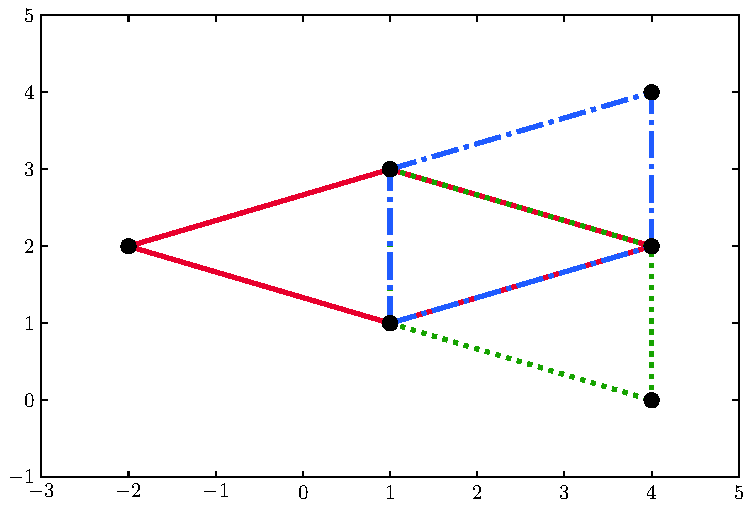
\includegraphics[width=1.0\textwidth]{i1/partiseci.1ex6.eps}
\end{center}

% QUESTION 7
\qs{I.1.7}{Describe the column space of \(A = 
\begin{bmatrix}
	\bm{v} & \bm{w} & \bm{v} + 2\bm{w} \\
\end{bmatrix}\). Describe the nullspace of \(A\): all vectors \(\bm{x} = \!\left( x_{1}, x_{2}, x_{3} \right) \) that solve \(A \bm{x} = \bm{0}\). Add the ``dimensions'' of that plane (the column space of \(A\)) and that line (the nullspace of \(A\)):
\[
	\textbf{dimension of column space}
\]
\[
	\bm{+}
\]
\[
	\textbf{dimension of nullspace}
\]
\[
	\textbf{=}
\]
\[
	\textbf{number of columns}
\]}

The column space of \(A\) is the set of all vectors of form
\[
	c_{1} \bm{v} + c_{2} \bm{w}
\]
Assuming independence of \(\bm{v}\) and \(\bm{w}\), the nullspace has basis
\[
	\bm{x} = \!\left( 1, 2, -1 \right) 
\]
with the nullspace constituting of all scalar multiples of \(\bm{x}\).

The formula given here is the Rank-Nullity Theorem. The basis of the column space has two independent vectors, while the basis of the nullspace has only one. The sum is the number of columns, three.

\vspace{12pt}

% QUESTION 8
\qs{I.1.8}{\(\bm{A} = \bm{CR}\) is a representation of the columns of \(A\) in the basis formed by the columns of \(C\) with coefficients in \(R\). If \(A_{ij} = j^{2}\) is 3 by 3, write down \(A\) and \(C\) and \(R\).}

By premise, \(A\) is
\[
	\begin{bmatrix}
		1 & 4 & 9 \\
		1 & 4 & 9 \\
		1 & 4 & 9 \\
	\end{bmatrix}
\]
with corresponding matrix factorization
\[
	\bm{A} = \bm{CR} = 
	\begin{bmatrix}
		1 \\
		1 \\
		1 \\
	\end{bmatrix}
\begin{bmatrix}
	1 & 4 & 9 \\
\end{bmatrix}
\]

% QUESTION 9
\qs{I.1.9}{Suppose the column space of an \(m\) by \(n\) matrix is all of \(\mathbb{R}^{3}\). What can you say about \(m\)? What can you say about \(n\)? What can you say about the rank \(r\)?}

We can decisively conclude that \(m = 3\). Additionally, we can conclude that \(n \ge 3\). The rank is \(r = 3\). The column space must have three independent vectors in its basis. 

\vspace{12pt}

% QUESTION 10
\qs{I.1.10}{Find the matrices \(C_{1}\) and \(C_{2}\) containing independent columns of \(A_{1}\) and \(A_{2}\):
\[
	A_{1} =
	\begin{bmatrix}
		1 & 3 & -2 \\
		3 & 9 & -6 \\
		2 & 6 & -4 \\
	\end{bmatrix}
\qquad
A_{2} = 
\begin{bmatrix}
	1 & 2 & 3 \\
	4 & 5 & 6 \\
	7 & 8 & 9 \\
\end{bmatrix}
\]}

We have
\[
	C_{1} =
	\begin{bmatrix}
		1 \\
		3 \\
		2 \\
	\end{bmatrix}
\qquad
C_{2} = A_{2}
\]

% QUESTION 11
\qs{I.1.11}{Factor each of those matrices into \(A = CR\). The matrix \(R\) will contain the numbers that multiply columns of \(C\) to recover columns of \(A\).

This is one way to look at matrix multiplication: 

\(\bm{C} \textbf{ times each column of } \bm{R}\).}

We have
\[
	A_{1} = C_{1} R_{1} =
	\begin{bmatrix}
		1 \\
		3 \\
		2 \\
	\end{bmatrix}
\begin{bmatrix}
	1 & 3 & -2 \\
\end{bmatrix}
\qquad
A_{2} = C_{2} R_{2} =
\begin{bmatrix}
	1 & 2 & 3 \\
	4 & 5 & 6 \\
	7 & 8 & 9 \\
\end{bmatrix}
\begin{bmatrix}
	1 & 0 & 0 \\
	0 & 1 & 0 \\
	0 & 0 & 1 \\
\end{bmatrix}
\]
% QUESTION 12
\qs{I.1.12}{Produce a basis for the column spaces of \(A_{1}\) and \(A_{2}\). What are the \textit{dimensions} of those column spaces -- the number of independent vectors? What are the \textit{ranks} of \(A_{1}\) and \(A_{2}\)? How many independent rows in \(A_{1}\) and \(A_{2}\)?}

The bases of \(A_{1}\) and \(A_{2}\) are the columns of \(C_{1}\) and \(C_{2}\). The dimensions are one and three, respectively. The ranks of \(A_{1}\) and \(A_{2}\) are one and three, respectively. Same for the number of independent rows in each.

\vspace{12pt}

% QUESTION 13
\qs{I.1.13}{Create a 4 by 4 matrix \(A\) of rank 2. What shapes are \(C \) and \(R\)?}

\[
	A = 
	\begin{bmatrix}
		1 & 2 & 3 & 0 \\
		0 & 0 & 0 & 0 \\
		0 & 0 & 0 & 1 \\
		0 & 0 & 0 & 1 \\
	\end{bmatrix}
\]
From \(A\), we derive \(C\) and \(R\) as
\[
	C =
	\begin{bmatrix}
		1 & 0 \\
		0 & 0 \\
		0 & 1 \\
		0 & 1 \\
	\end{bmatrix}
\qquad
	R = 
	\begin{bmatrix}
		1 & 2 & 3 & 0 \\
		0 & 0 & 0 & 1 \\
	\end{bmatrix}
\]

% QUESTION 14
\qs{I.1.14}{Suppose two matrices \(A\) and \(B\) have the same column space.
\begin{enumerate}[label=(\alph*)]
	\item Show that their row spaces can be different.
	\item Show that the matrices \(C\) (basic columns) can be different.
	\item What number will be the same for \(A\) and \(B\)?
\end{enumerate}}

(a) Consider \(A\) and \(B\) each with basis of dimension \(n\) that spans \(\mathbb{R}^{n}\). Further suppose that one of the matrices has a greater number of columns than the other. Then the row spaces can \textit{never} be the same.

(b) Suppose we have
\[
	A = 
	\begin{bmatrix}
		1 & 0 \\
		0 & 1 \\
	\end{bmatrix}
	\qquad
	B = 
	\begin{bmatrix}
		1 & 1 \\
		0 & 1 \\
	\end{bmatrix}
\]
Each matrix has a basis that spans \(\mathbb{R}^{2}\). Yet the matrices \(C\) (each of \(A\)'s and \(B\)'s column matrices equal to itself) differ.

(c) The rank, as both \(A\) and \(B\) must share the same number of independent column vectors to share the same column space.

\vspace{12pt}

% QUESTION 15
\qs{I.1.15}{If \(A = CR\), the first row of \(A\) is a combination of the rows of \(R\). Which part of which matrix holds the coefficients in that combination -- the numbers that multiply the rows of \(R\) to produce row 1 of \(A\)?}

The first row of the column matrix \(C\) is the linear combination of rows of \(R\) to produce the first row of \(A\).

\vspace{12pt}

% QUESTION 16
\qs{I.1.16}{The rows of \(R\) are a basis for the row space of \(A\). \textit{What does that sentence mean}?}

One way to conceptualize the \textbf{basis} is the minimally viable ``ingredients'' to generate the entirety of the row space. Put differently, the basis is the set of independent vectors that, when put into any linear combination, can be made to yield \textit{any} arbitrary vector in that space. 

Rigorously, if \(\left\{ \bm{v_{1}}, \ldots, \bm{v_{n}}\right\} \) form a basis for a vector space \(\mathbb{V}\), then for \textit{any} vector \(\bm{v} \in \mathbb{V}\), we can find coefficients \(c_{1}, \ldots, c_{n} \in \mathbb{R}\) such that
\[
	c_{1} \bm{v_{1}} + \cdots + c_{n} \bm{v_{n}} = \bm{v}
\]
\newpage
% QUESTION 17
\qs{I.1.17}{For these matrices with square blocks, find \(A = CR\). What ranks?

\[
	A_{1} =
	\begin{bmatrix}
		\text{zeros} & \text{ones} \\
		\text{ones} & \text{ones} \\
	\end{bmatrix}_{\bm{4 \times 4}}
\qquad
	A_{2} = 
	\begin{bmatrix}
		A_{1} \\
		A_{1} \\
	\end{bmatrix}_{\bm{8 \times 4}}
\qquad
	A_{3} = 
	\begin{bmatrix}
		A_{1} & A_{1} \\
		A_{1} & A_{1} \\
	\end{bmatrix}_{\bm{8 \times 8}}
\]}
\[
	A_{1} = C_{1}R_{1} =
	\begin{bmatrix}
		0 & 1 \\
		0 & 1 \\
		1 & 1 \\
		1 & 1 \\
	\end{bmatrix}
	\begin{bmatrix}
		1 & 1 & 0 & 0 \\
		0 & 0 & 1 & 1 \\
	\end{bmatrix},
	\quad
	\text{rank}\!\left( A_{1} \right)  = 2
\]
\[
	A_{2} = C_{2} R_{2} = 
	\begin{bmatrix}
		C_{1} \\
		C_{1} \\
	\end{bmatrix}
	\begin{bmatrix}
		R_{1} \\
	\end{bmatrix},
	\quad
	\text{rank}\!\left( A_{2} \right) = 2
\]
\[
	A_{3} = C_{3}R_{3} =
	\begin{bmatrix}
		C_{1} \\
		C_{1} \\
	\end{bmatrix}
	\begin{bmatrix}
		R_{1} & R_{1} \\
	\end{bmatrix},
	\quad
	\text{rank}\!\left( A_{3} \right) = 2
\]

% QUESTION 18
\qs{I.1.18}{If \(A = CR\), what are the \(CR\) factors of the matrix \(
\begin{bmatrix}
	0 & A \\
	0 & A \\
\end{bmatrix} \)?}

We have
\[
	\begin{bmatrix}
		0 & A \\
		0 & A \\
	\end{bmatrix}
	=
	\begin{bmatrix}
		C \\
		C \\
	\end{bmatrix}
	\begin{bmatrix}
		0 & R \\
	\end{bmatrix}
\]

% QUESTION 19
\qs{I.1.19}{``Elimination'' subtracts a number \(l_{ij}\) times row \(j\) from row \(i\): a ``row operation.'' Show how those steps can reduce the matrix \(A\) in Example 4 to \(R\) (except that this row echelon form \(R\) has a row of zeros). The rank won't change!
\[
	A = 
	\begin{bmatrix}
		1 & 3 & 8 \\
		1 & 2 & 6 \\
		0 & 1 & 2 \\
	\end{bmatrix}
	\rightarrow
	\quad
	\rightarrow
	\quad
	R =
	\begin{bmatrix}
		1 & 0 & 2 \\
		0 & 1 & 2 \\
		0 & 0 & 0 \\
	\end{bmatrix}
	= \textbf{rref}\!\left( A \right). 
\]}

Subtract row 1 from row 2:
\[
	E_{1} = 
	\begin{bmatrix}
		1 & 3 & 8 \\
		0 & -1 & -2 \\
		0 & 1 & 2 \\
	\end{bmatrix}
\]

Add row 2 to row 3:
\[
	E_{2} = 
	\begin{bmatrix}
		1 & 3 & 8 \\
		0 & -1 & -2 \\
		0 & 0 & 0 \\
	\end{bmatrix}
\]
Multiply row 2 by 3, and then add to row 1:
\[
	E_{3} = 
	\begin{bmatrix}
		1 & 0 & 2 \\
		0 & -1 & -2 \\
		0 & 0 & 0 \\
	\end{bmatrix}
\]
Lastly, multiply row 2 by \(-1\):
\[
	R = 
	\begin{bmatrix}
		1 & 0 & 2 \\
		0 & 1 & 2 \\
		0 & 0 & 0 \\
	\end{bmatrix}
\]
\newpage
\subsection{\textsf{I.2 - Matrix-Matrix Multiplication \texorpdfstring{\(\bm{AB}\)}{AB}}}

% QUESTION 1
\qs{I.2.1}{Suppose \(A \bm{x} = \bm{0}\) and \(A \bm{y} = \bm{0}\) (where \(\bm{x}\) and \(\bm{y}\) and \(\bm{0}\) are vectors). Put those two statements together into one matrix equation \(AB = C\). What are those matrices \(B\) and \(C\)? If the matrix \(A\) is \(m\) by \(n\), what are the shapes of \(B\) and \(C\)?}

We may write
\[
	AB = 
	A
	\begin{bmatrix}
		\bm{x} & \bm{y} \\
	\end{bmatrix}
        =
	\begin{bmatrix}
		\bm{0} & \bm{0} \\
	\end{bmatrix}
	= C
\]
where \(B\) is \(n\) by \(2\) and \(C\) is \(m\) by \(2\).

\vspace{12pt}

% QUESTION 2
\qs{I.2.2}{Suppose \(\bm{a}\) and \(\bm{b}\) are column vectors with components \(a_{1}, \ldots, a_{m}\) and \(b_{1}, \ldots, b_{p}\). Can you multiply \(\bm{a}\) times \(\bm{b}^{\textsc{T}}\) (yes or no)? What is the shape of the answer \(\bm{ab}^{\textsc{T}}\)? What number is in row \(i\), column \(j\) of \(\bm{ab}^{\textsc{T}}\)? What can you say about \(\bm{aa}^{\textsc{T}}\)?}

Yes, as \(\bm{a}\) has shape \(m\) by \(1\) and \(\bm{b}^{\textsc{T}}\) has shape \(1\) by \(p\). The shape of \(\bm{ab}^{\textsc{T}}\) is \(m\) by \(p\). The \(ij\)-th element of \(\bm{ab}^{\textsc{T}}\) is
\[
	a_{i}b_{j}
\]
The matrix \(\bm{aa}^{\textsc{T}}\) is rank 1. It is also symmetric, as \(\bm{aa}^{\textsc{T}} = \!\left( \bm{aa}^{\textsc{T}} \right)^{\textsc{T}}\).

\vspace{12pt}

% QUESTION 3
\qs{I.2.3}{(Extension of Problem \textbf{2}: Practice with subscripts) Instead of that one vector \(\bm{a}\), suppose you have \(n\) vectors \(\bm{a}_{1}\) to \(\bm{a}_{n}\) in the columns of \(A\). Suppose you have \(n\) vectors \(\bm{b}_{1}^{\textsc{T}}, \ldots, \bm{b}_{n}^{\textsc{T}}\) in the rows of \(B\).

\begin{enumerate}[label=(\alph*)]
	\item Give a ``sum of rank one'' formula for the matrix-matrix product \(AB\).
	\item Give a formula for the \(i\), \(j\) entry of that matrix-matrix product \(AB\). Use sigma notation to add the \(i\), \(j\) entries of each matrix \(\bm{a}_{k}\bm{b}_{k}^{\textsc{T}}\), found in Problem 2.
\end{enumerate}}

(a)

\[
	AB = \bm{a}_{1}\bm{b}_{1}^{\textsc{T}} + \bm{a}_{2}\bm{b}_{2}^{\textsc{T}} + \cdots + \bm{a}_{n}\bm{b}_{n}^{\textsc{T}}
\]
(b)

\[
	AB_{ij} = \sum_{k=1}^{n} a_{ik}b_{kj}^{\textsc{T}}
\]
where \(a_{ik}b_{kj}^{\textsc{T}}\) is the \(ij\)-th element in the \(k\)-th rank 1 matrix in the sum in part (a).

\vspace{12pt}

% QUESTION 4
\qs{I.2.4}{Suppose \(B\) has only one column \(\!\left( p = 1 \right) \). So each row of \(B\) just has one number. \(A\) has columns \(\bm{a}_{1}\) to \(\bm{a}_{n}\) as usual. Write down the column times row formula for \(AB\). In words, the \(m\) by \(1\) column vector \(AB\) is the combination of the \underline{\qquad}.}

If \(B\) is
\[
	\begin{bmatrix}
		b_{1} \\
		b_{2} \\
		\vdots  \\
		b_{n} \\
	\end{bmatrix}
\]
Then we have
\[
	AB = \sum_{k=1}^{n} \bm{a}_{k}b_{k} 
\]
where we multiply each column of \(A\) by each corresponding scalar element of \(B\).

\vspace{12pt}

% QUESTION 5
\qs{I.2.5}{Start with a matrix \(B\). If we want to take combinations of its rows, we premultiply by \(A\) to get \(AB\). If we want to take combinations of its columns, we postmultiply by \(C\) to get \(BC\). For this question we will do both.

\begin{center}
	\resizebox{\textwidth}{!}{%
\begin{tabular}{cc}
	\textbf{Row operations then column operations} & First \(AB\) then \(\!\left( AB \right) C\) \\
	\textbf{Column operations then row operations} & First \(BC\) then \(A \!\left( BC \right) \) \\
\end{tabular}}
\end{center}
The \textbf{associative law} says that we get the same final result both ways.

Verify \(\bm{\!\left( AB \right) C = A \!\left( BC \right) }\) \text{ for}
\[
	A = 
	\begin{bmatrix}
		1 & a \\
		0 & 1 \\
	\end{bmatrix}
	\quad
	B = 
	\begin{bmatrix}
		b_{1} & b_{2} \\
		b_{3} & b_{4} \\
	\end{bmatrix}
	\quad
	C = 
	\begin{bmatrix}
		1 & 0 \\
		c & 1 \\
	\end{bmatrix}
\]}

\begin{align*}
	\!\left( AB \right) C & =
	\!\left( 
	\begin{bmatrix}
		1 & a \\
		0 & 1 \\
	\end{bmatrix}
	\begin{bmatrix}
		b_{1} & b_{2} \\
		b_{3} & b_{4} \\
	\end{bmatrix}
	\right) 
	\begin{bmatrix}
		1 & 0 \\
		c & 1 \\
	\end{bmatrix} \\
	& =
	\begin{bmatrix}
		b_{1} + a b_{3} & b_{2} + ab_{4} \\
		b_{3} & b_{4} \\
	\end{bmatrix}
	\begin{bmatrix}
		1 & 0 \\
		c & 1 \\
	\end{bmatrix} \\
	& =
	\begin{bmatrix}
		b_{1} + ab_{3} + b_{2}c + ab_{4}c & b_{2} + ab_{4} \\
		b_{3} + b_{4}c & b_{4} \\
	\end{bmatrix} \\
	A \!\left( BC \right) & =
	\begin{bmatrix}
		1 & a \\
		0 & 1 \\
	\end{bmatrix}
	\!\left( 
	\begin{bmatrix}
		b_{1} & b_{2} \\
		b_{3} & b_{4} \\
	\end{bmatrix}
	\begin{bmatrix}
		1 & 0 \\
		c & 1 \\
	\end{bmatrix}
	\right) \\
	& = 
	\begin{bmatrix}
		1 & a \\
		0 & 1 \\
	\end{bmatrix}
	\begin{bmatrix}
		b_{1} + b_{2}c & b_{2} \\
		b_{3} + b_{4}c & b_{4} \\
	\end{bmatrix} \\
	& =
	\begin{bmatrix}
		b_{1} + b_{2}c + ab_{3} + ab_{4}c & b_{2} + ab_{4} \\
		b_{3} + b_{4}c & b_{4} \\
	\end{bmatrix}
\end{align*}

Ascertaining that \(\!\left( AB \right) C = A \!\left( BC \right) \).

\vspace{12pt}

% QUESTION 6
\qs{I.2.6}{If \(A\) has columns \(\bm{a}_{1}\), \(\bm{a}_{2}\), \(\bm{a}_{3}\) and \(B = I\) is the identity matrix, what are the rank one matrices \(\bm{a}_{1}\bm{b}_{1}^{*}\) and \(\bm{a}_{2}\bm{b}_{2}^{*}\) and \(\bm{a}_{3}\bm{b}_{3}^{*}\)? They should add to \(AI = A\).}

We have
\begin{align*}
	\bm{a}_{1}\bm{b}_{1}^{*} & =
	\bm{a}_{1} 
	\begin{bmatrix}
		1 & 0 & 0 \\
	\end{bmatrix} \\
	  & =
	\begin{bmatrix}
		\bm{a}_{1} & \bm{0} & \bm{0} \\
	\end{bmatrix} \\
	\bm{a}_{2}\bm{b}_{2}^{*} & =
	\bm{a}_{2}
	\begin{bmatrix}
		0 & 1 & 0 \\
	\end{bmatrix} \\
	& =
	\begin{bmatrix}
		\bm{0} & \bm{a}_{2} & \bm{0}  \\
	\end{bmatrix} \\
	\bm{a}_{3}\bm{b}_{3}^{*} & = \bm{a}_{3}
	\begin{bmatrix}
		0 & 0 & 1 \\
	\end{bmatrix} \\
	& =
	\begin{bmatrix}
		\bm{0} & \bm{0} & \bm{a}_{3} \\
	\end{bmatrix}
\end{align*}

Therefore, the sum
\[
	\sum_{k=1}^{3} \bm{a}_{k}\bm{b}_{k}^{*}
\]
is equal to
\[
	A =
	\begin{bmatrix}
		\bm{a}_{1} & \bm{a}_{2} & \bm{a}_{3} \\
	\end{bmatrix}
\]
Hence \(AI = A\).

\vspace{12pt}

% QUESTION 7
\qs{I.2.7}{\textit{Fact}: The columns of \(AB\) are combinations of the columns of \(A\). Then the column \textit{space} of \(AB\) is \textit{contained in} the column space of \(A\). Give an example of \(A\) and \(B\) for which \(AB\) has a smaller column space than \(A\).}

Define \(A\) and \(B\) as
\[
	A =
	\begin{bmatrix}
		1 & 1 \\
		0 & 1 \\
	\end{bmatrix}
	\qquad
	B = 
	\begin{bmatrix}
		1 & 0 \\
		0 & 0 \\
	\end{bmatrix}
\]

Then
\[
	AB =
	\begin{bmatrix}
		1 & 0 \\
		0 & 0 \\
	\end{bmatrix}
\]
Since \(\text{rank}\!\left( A \right) = 2\) and \(\text{rank}\!\left( AB \right) = 1\), we can definitively say that \(\textbf{C}\!\left( A \right) \neq \textbf{C}\!\left( AB \right) \). 

\vspace{12pt}

\newpage
% QUESTION 8
\qs{I.2.8}{To compute \(C = AB = \!\left( m \text{ by } n \right) \!\left( n \text{ by } p \right) \), what order of the same three commands leads to columns times rows (outer products)?

\begin{tabular}{ccc}
	\textbf{Rows times columns} & \qquad & \textbf{Columns times rows} \\
	For \(i = 1\) to \(m\) & \qquad & For \(\ldots\) \\
	For \(j = 1\) to \(p\) & \qquad & For \(\ldots\) \\
	For \(k = 1\) to \(n\) & \qquad & For \(\ldots\) \\
	\(C \!\left( i,j \right) = C \!\left( i,j \right) + A \!\left( i, k \right) * B \!\left( k,j \right) \) & \qquad & \(C = \) \\
\end{tabular}}

We have

\begin{center}
\begin{tabular}{c}
	\textbf{Rows times columns} \\
	For \(k = 1\) to \(n\) \\
	For \(i = 1\) to \(m\) \\
	For \(j = 1\) to \(p\) \\
\end{tabular}
\end{center}

\newpage
\subsection{\textsf{I.3 - The Four Fundamental Subspaces}}

% QUESTION 1
\qs{I.3.1}{Show that the nullspace of \(AB\) contains the nullspace of \(B\). }

The nullspace of \(AB\) is the set of \(\bm{x}\) such that 
\[
	AB \bm{x} = \bm{0}
\]
Therefore, if \(B \bm{x} = \bm{0}\), it must also be the cause that if \(\bm{x} \in \textbf{N}\!\left( B \right) \), it immediately implies that \(\bm{x} \in \textbf{N}\!\left( AB \right) \).

\vspace{12pt}

% QUESTION 2
\qs{I.3.2}{Find a square matrix with \(\text{rank}\!\left( A^{2} \right) < \text{rank} \!\left( A \right) \). Confirm that \(\text{rank} \!\left( A^{\textsc{T}}A \right) = \text{rank}\!\left( A \right) \).}

Consider the matrix
\[
	A = 
	\begin{bmatrix}
		0 & 1 \\
		0 & 0 \\
	\end{bmatrix}
\]
from which we have \(\text{rank}\!\left( A \right) = 1\). However, we also have
\[
	A^{2} =
	\begin{bmatrix}
		0 & 0 \\
		0 & 0 \\
	\end{bmatrix}
\]
Thus \(\text{rank}\!\left( A^{2} \right) = 0\). On the other hand, we have
\[
	A^{\textsc{T}}A = 
	\begin{bmatrix}
		0 & 0 \\
		1 & 0 \\
	\end{bmatrix}
	\begin{bmatrix}
		0 & 1 \\
		0 & 0 \\
	\end{bmatrix}
	=
	\begin{bmatrix}
		0 & 0 \\
		0 & 1 \\
	\end{bmatrix}
\]
with \(\text{rank}\!\left( A^{\textsc{T}}A \right) = 1\), ascertaining that \(\text{rank}\!\left( A^{\textsc{T}}A \right) = \text{rank}\!\left( A \right) \).

\vspace{12pt}

% QUESTION 3
\qs{I.3.3}{How is the nullspace of \(C\) related to the nullspaces of \(A\) and \(B\), if \(C =
\begin{bmatrix}
	A \\
	B \\
\end{bmatrix}\)?}

We have \(\textbf{N}\!\left( C \right) = \textbf{N}\!\left( A \right) \cap \textbf{N}\!\left( B \right) \). The reasoning is as follows: let \(\bm{x} \in \textbf{N} \!\left( C \right) \). To be clear, we wish to solve the matrix equation
\[
	C \bm{x} = 
	\begin{bmatrix}
		\bm{a}_{1} & \bm{a}_{2} & \cdots  & \bm{a}_{n} \\
		\bm{b}_{1} & \bm{b}_{2} & \cdots  & \bm{b}_{n} \\
	\end{bmatrix}
	\bm{x} = \bm{0}
\]
In doing so, \(\bm{x}\) must combine the columns of \(C\) in such a way that the sums of \(\bm{a}_{1}, \ldots, \bm{a}_{n}\) \textit{and} \(\bm{b}_{1}, \ldots, \bm{b}_{n}\) vanish. The only such \(\bm{x}\) to do so \textit{must} exist in both \(\textbf{N}\!\left( A \right) \) and \(\textbf{N}\!\left( B \right) \).

\vspace{12pt}

% QUESTION 4
\qs{I.3.4}{If row space of \(A = \) column space of \(A\), and also \(\textbf{N}\!\left( A \right) = \textbf{N} \!\left( A^{\textsc{T}} \right) \), is \(A\) symmetric?}

No. Consider the counterexample of a non-elementary \(4 \times 4\) permutation matrix:
\[
	A =
	\begin{bmatrix}
		0 & 1 & 0 & 0 \\
		0 & 0 & 1 & 0 \\
		0 & 0 & 0 & 1 \\
		1 & 0 & 0 & 0 \\
	\end{bmatrix}
\]
which has transpose
\[
	A^{\textsc{T}} =
	\begin{bmatrix}
		0 & 0 & 0 & 1 \\
		1 & 0 & 0 & 0 \\
		0 & 1 & 0 & 0 \\
		0 & 0 & 1 & 0 \\
	\end{bmatrix}
\]
So clearly \(A\) is non-symmetric. However, \(\text{rank}\!\left( A \right) = 4\), meaning the row and column spaces are \(\mathbb{R}^{4}\). Additionally, \(\textbf{N}\!\left( A \right) \) and \(\textbf{N}\!\left( A^{\textsc{T}} \right) \) are the same (consisting only of the zero vector). Ergo, it need not hold that a matrix \(A\) with such properties be symmetric.

\vspace{12pt}

% QUESTION 5
\qs{I.3.5}{Four possibilities for the rank \(r\) and size \(m\), \(n\) match four possibilities for \(A \bm{x} = b\). Find four matrices \(A_{1}\) to \(A_{4}\) that show those possibilities:

\begin{center}
\begin{tabular}{|ll|}
	\hline
	\(\bm{r = m = n}\) & \(A_{1} \bm{x} = \bm{b}\) has \textbf{1 solution for every \(\bm{b}\)} \\
	\(\bm{r = m < n}\) & \(A_{2}\bm{x} = \bm{b}\) has \textbf{\(\bm{\infty}\) solutions for every \(\bm{b}\)} \\
	\(\bm{r = n < m}\) & \(A_{3}\bm{x} = \bm{b}\) has \textbf{0 or 1 solution} \\
	\(\bm{r < m}\), \(\bm{r < n}\) & \(A_{4}\bm{x} = \bm{b}\) has \textbf{0 or \(\bm{\infty}\) solutions} \\
	\hline
\end{tabular}
\end{center}}

Examples of these matrices and solutions to the matrix equation are:
\begin{align*}
	A_{1} & =
	\begin{bmatrix}
		1 & 0 \\
		0 & 1 \\
	\end{bmatrix},
	\quad
	\bm{b} =
	\begin{bmatrix}
		b_{1} \\
		b_{2} \\
	\end{bmatrix},
	\quad
	\bm{x} =
	\begin{bmatrix}
		b_{1} \\
		b_{2} \\
	\end{bmatrix} \\
	A_{2} & =
	\begin{bmatrix}
		1 & 0 & 1 \\
		0 & 1 & 1 \\
	\end{bmatrix},
	\quad
	\bm{b} =
	\begin{bmatrix}
		b_{1} \\
		b_{2} \\
	\end{bmatrix},
	\quad
	\bm{x} =
	\begin{bmatrix}
		c + b_{1} \\
		c + b_{2} \\
		-c \\
	\end{bmatrix} \text{for any } c \in \mathbb{R} \\
	A_{3} & =
	\begin{bmatrix}
		1 & 0 \\
		0 & 1 \\
		1 & 1 \\
	\end{bmatrix},
	\quad
	\bm{b} =
	\begin{bmatrix}
		b_{1} \\
		b_{2} \\
		b_{3} \\
	\end{bmatrix},
	\quad
	\bm{x} =
	\begin{bmatrix}
		b_{1} \\
		b_{2} \\
	\end{bmatrix} \text{(solution only if } b_{1} + b_{2} = b_{3} \text{)} \\
	A_{4} & =
	\begin{bmatrix}
		1 & 0 \\
		0 & 0 \\
	\end{bmatrix},
	\quad
	\bm{b} =
	\begin{bmatrix}
		b_{1} \\
		b_{2} \\
	\end{bmatrix},
	\quad
	\bm{x} = 
	\begin{bmatrix}
		b_{1} \\
		c \\
	\end{bmatrix} \text{(if \(b_{2} = 0\), \(\infty\) sols, otherwise 0 sols)}
\end{align*}

% QUESTION 6
\qs{I.3.6}{(\textit{Important}) Show that \(\bm{A^{\textsc{T}}A}\) \textbf{has the same nullspace as} \(\bm{A}\). Here is one approach:

First, if \(A \bm{x}\) equals zero then \(A^{\textsc{T}}A \bm{x}\) equals \underline{\qquad}. This proves \(\textbf{N}\!\left( A \right) \subset \textbf{N}\!\left( A^{\textsc{T}}A \right) \).

Second, if \(A^{\textsc{T}}A \bm{x} = \bm{0}\) then \(\bm{x}^{\textsc{T}}A^{\textsc{T}}A \bm{x} = \abs{\abs{A \bm{x}}}^{2} = 0\). Deduce \(\textbf{N}\!\left( A^{\textsc{T}}A \right) = \textbf{N}\!\left( A \right) \).}

First, suppose that \(A \bm{x} = \bm{0}\). Then we have \(A^{\textsc{T}}A \bm{x} = \bm{0}\). Equivalently, \(\bm{x} \in \textbf{N}\!\left( A \right) \) implies \(\bm{x} \in \textbf{N}\!\left( A^{\textsc{T}}A \right) \), so \(\textbf{N}\!\left( A \right) \subset \textbf{N}\!\left( A^{\textsc{T}}A \right) \).  Now suppose that \(A^{\textsc{T}}A \bm{x} = \bm{0}\) or \(\bm{x} \in \textbf{N}\!\left( A^{\textsc{T}}A \right) \). Then left-multiplication by \(\bm{x}^{\textsc{T}}\) gives us
\[
	\bm{x}^{\textsc{T}}A^{\textsc{T}}A \bm{x} = \abs{\abs{A \bm{x}}}^{2} = 0
\]
which implies that the norm of \(A \bm{x}\) is zero; ergo, \(A \bm{x} = \bm{0}\) and \(\bm{x} \in \textbf{N}\!\left( A \right) \). Then \(\textbf{N}\!\left( A^{\textsc{T}}A \right) \subset \textbf{N}\!\left( A \right) \), enabling us to conclude \(\textbf{N}\!\left( A^{\textsc{T}}A \right) = \textbf{N}\!\left( A \right) \). 

\vspace{12pt}

% QUESTION 7
\qs{I.3.7}{Do \(A^{2}\) and \(A\) always have the same nullspace? \(A\) is a square matrix.}

No. Consider the example given in exercise 2, where \(\text{rank}\!\left( A^{2} \right) < \text{rank}\!\left( A \right) \). Here, \(\text{rank}\!\left( A^{2} \right) = 0\) and \(\text{rank}\!\left( A \right) = 1\). Since both are \(2 \times 2\), by the rank-nullity theorem, the nullities differ, and thus they cannot have the same nullspace.

\vspace{12pt}

% QUESTION 8
\qs{I.3.8}{Find the column space \(\textbf{C}\!\left( A \right) \) and the nullspace \(\textbf{N}\!\left( A \right) \) of \(A = 
\begin{bmatrix}
	\bm{0} & \bm{1} \\
	\bm{0} & \bm{0} \\
\end{bmatrix}\). Remember that those are vector spaces, not just single vectors. This is an unusual example with \(\textbf{C}\!\left( A \right) = \textbf{N}\!\left( A \right) \). It could not happen that \(\textbf{C}\!\left( A \right) = \textbf{N}\!\left( A^{\textsc{T}} \right) \) because those two subspaces are orthogonal.}

We have 
\[
	\textbf{C}\!\left( A \right) = \left\{ \bm{x} \ :\bm{x} = 
	\begin{bmatrix}
		c \\
		0 \\
	\end{bmatrix}, c \in \mathbb{R}
	\right\} 
\]
and \(\textbf{N}\!\left( A \right) \) is equivalently defined.

\vspace{12pt}

\newpage
% QUESTION 9
\qs{I.3.9}{Draw a square and connect its corners to the center point: 5 nodes and 8 edges. Find the 8 by 5 incidence matrix \(A\) of this graph (rank \(r = 5 - 1 = 4\)). Find a vector \(\bm{x}\) in \(\textbf{N}\!\left( A \right) \) and \(8 - 4\) independent vectors \(\bm{y}\) in \(\textbf{N}\!\left( A^{\textsc{T}} \right) \).}

One graph we may draw is

\begin{center}
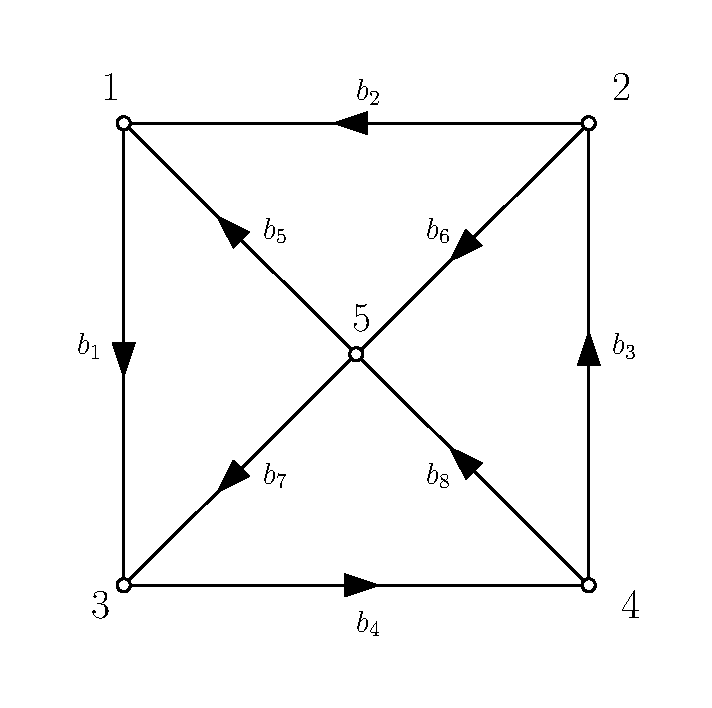
\includegraphics[width=0.5\textwidth]{i3/partiseci.3ex9.eps}
\end{center}

The corresponding incidence matrix is
\[
	\begin{bmatrix}
		-1 & 0 & 1 & 0 & 0 \\
		1 & -1 & 0 & 0 & 0 \\
		0 & 1 & 0 & -1 & 0 \\
		0 & 0 & -1 & 1 & 0 \\
		1 & 0 & 0 & 0 & -1 \\
		0 & -1 & 0 & 0 & 1 \\
		0 & 0 & 1 & 0 & -1 \\
		0 & 0 & 0 & -1 & 1 \\
	\end{bmatrix}
\]
One vector \(\bm{x} \in \textbf{N}\!\left( A \right) \) is given by
\[
	\bm{x} = 
	\begin{bmatrix}
		1 \\
		1 \\
		1 \\
		1 \\
		1 \\
	\end{bmatrix}
\]
Four vectors in \(\textbf{N}\!\left( A^{\textsc{T}} \right) \) are
\[
	\bm{x}_{1} =
	\begin{bmatrix}
		0 \\
		0 \\
		0 \\
		1 \\
		0 \\
		0 \\
		1 \\
		1 \\
	\end{bmatrix},
	\quad
	\bm{x}_{2} =
	\begin{bmatrix}
		1 \\
		1 \\
		1 \\
		1 \\
		0 \\
		0 \\
		0 \\
		0 \\
	\end{bmatrix},
	\quad
	\bm{x}_{3} =
	\begin{bmatrix}
		1 \\
		0 \\
		0 \\
		1 \\
		1 \\
		0 \\
		0 \\
		1 \\
	\end{bmatrix},
	\quad
	\bm{x}_{4} =
	\begin{bmatrix}
		0 \\
		0 \\
		1 \\
		1 \\
		0 \\
		1 \\
		1 \\
		0 \\
	\end{bmatrix}
\]

% QUESTION 10
\qs{I.3.10}{If \(\textbf{N}\!\left( A \right) \) is the zero vector, what vectors are in the nullspace of \(B = 
\begin{bmatrix}
	A & A & A \\
\end{bmatrix} \)?}

First we must critically observe that if \(A\) has rank \(n\), then \(B\) also has rank \(n\). In particular, \(B\) has infinitely many solutions to \(B \bm{x} = \bm{0}\). We have in \(\textbf{N}\!\left( B \right) \) vectors of the form:
\[
	\bm{x} =
	\begin{bmatrix}
		\bm{b}_{1} \\
		\bm{b}_{2} \\
		\bm{b}_{3} \\
	\end{bmatrix}
\]
where the components of \(\bm{b}_{1}\), \(\bm{b}_{2}\), and \(\bm{b}_{3}\) are chosen in such a way that the columns of \(B\) sum to zero. 

\vspace{12pt}

% QUESTION 11
\qs{I.3.11}{For subspaces \textbf{S} and \textbf{T} of \(\mathbb{R}^{10}\) with dimensions 2 and 7, what are all the possible dimensions of
\begin{enumerate}[label=(\roman*)]
	\item \(\textbf{S} \cap \textbf{T} = \left\{ \text{all vectors that are in both subspaces} \right\} \)
	\item \(\textbf{S} + \textbf{T} = \left\{ \text{all sums \(s + t\) with \(s\) in \textbf{S} and \(t\) in \textsf{T}} \right\} \)
	\item \(\textbf{S}^{\bm{\perp}} = \left\{ \text{all vectors in \(\mathbb{R}^{10}\) that are \(\perp\) to every vector in \textbf{S}} \right\} \).
\end{enumerate}}

(i) Dimension equals 0, 1, or 2. Intuitively, consider \textbf{S} and \textbf{T} completely orthogonal to one another. Then \(\dim \!\left( \textbf{S} \cap  \textbf{T} \right) = 0 \). Alternatively, if \textbf{S} and \textbf{T} have one ``overlapping" dimension, \(\dim \!\left( \textbf{S} \cap \textbf{T} \right) = 1\). Analogously for two overlapping dimensions.

\vspace{12pt}

(ii) Dimension equals 7, 8, or 9. Imagine two independent vectors in three-dimensional space summed. The very act of summing takes us from the one dimension of the first vector to two dimensions. We may motivate this logic to say that \textbf{adding vectors that are independent of those in our subspace increases the dimension of the sum of subspaces.} Similarly, we appeal to the intuition of overlapping dimensions. If \textbf{S} is itself a subspace of \textbf{T} (i.e. \textbf{S} completely overlaps with \textbf{T}), then \(\dim \!\left( \textbf{S} + \textbf{T} \right) = 7\). In the alternative, if we have only one overlapping dimension, then the dimension of the subspace sum goes up to 8, and two overlapping dimensions leads to 9. 

\vspace{12pt}

(iii) Dimension equals 8. Intuitively, we wish to find the subspace of \(\mathbb{R}^{10}\) that is spanned by vectors completely independent of \textbf{S}. It must be the case that that subspace \(\textbf{S}^{\bm{\perp}}\) has dimension 8. In general, for \(\mathbb{R}^{n}\) and subspaces \(A\), \(A^{\perp}\), we have
\[
	\dim A + \dim A^{\perp} = n
\]

\newpage
\subsection{\textsf{I.4 - Elimination and \texorpdfstring{\(\bm{A = LU}\)}{A = LU}}}

% QUESTION 1
\qs{I.4.1}{Factor these matrices into \(A = LU\):
\[
	A = 
	\begin{bmatrix}
		2 & 1 \\
		6 & 7 \\
	\end{bmatrix}
	\quad
	A = 
	\begin{bmatrix}
		1 & 1 & 1 \\
		1 & 1 & 1 \\
		1 & 1 & 1 \\
	\end{bmatrix}
	\quad
	A = 
	\begin{bmatrix}
		2 & -1 & 0 \\
		-1 & 2 & -1 \\
		0 & -1 & 2 \\
	\end{bmatrix}
\]}

We have
\[
	A = 
	\begin{bmatrix}
		2 & 1 \\
		6 & 7 \\
	\end{bmatrix}
	=
	\begin{bmatrix}
		1 & 0 \\
		3 & 1 \\
	\end{bmatrix}
	\begin{bmatrix}
		2 & 1 \\
		0 & 4 \\
	\end{bmatrix}
\]
\[
	A = 
	\begin{bmatrix}
		1 & 1 & 1 \\
		1 & 1 & 1 \\
		1 & 1 & 1 \\
	\end{bmatrix}
	=
	\begin{bmatrix}
		1 & 0 & 0 \\
		1 & 1 & 0 \\
		1 & 0 & 1 \\
	\end{bmatrix}
	\begin{bmatrix}
		1 & 1 & 1 \\
		0 & 0 & 0 \\
		0 & 0 & 0 \\
	\end{bmatrix}
\]
\[
	A = 
	\begin{bmatrix}
		2 & -1 & 0 \\
		-1 & 2 & -1 \\
		0 & -1 & 2 \\
	\end{bmatrix}
	=
	\begin{bmatrix}
		1 & 0 & 0 \\
		-1/2 & 1 & 0 \\
		0 & -2/3 & 1 \\
	\end{bmatrix}
	\begin{bmatrix}
		2 & -1 & 0 \\
		0 & 3/2 & -1 \\
		0 & 0 & 4/3 \\
	\end{bmatrix}
\]

% QUESTION 2
\qs{I.4.2}{If \(a_{11}, \ldots, a_{1n}\) is the first row of a rank-1 matrix \(A\) and \(a_{11}, \ldots, a_{m1}\) is the first column, \textit{find a formula for} \(a_{ij}\). Good to check when \(a_{11} = 2\), \(a_{12} = 3\), \(a_{21} = 4\). When will your formula break down?}

We have
\[
	a_{ij} = \frac{a_{i1}a_{1j}}{a_{11}}
\]
Given the matrix
\[
	A = 
	\begin{bmatrix}
		2 & 3 \\
		4 & ? \\
	\end{bmatrix}
\]
In order to maintain \(\text{rank}\!\left( A \right) = 1\), we must have \(a_{22} = 6\). By our formula, we can derive
\[
	a_{22} = \frac{a_{21} a_{12}}{a_{11}} = \frac{4 \cdot 3}{2} = 6
\]
The problem that arises is if \(a_{11} = 0\). We can permute \(A\) such that the pivot in the first row is non-zero (and ideally largest).

\vspace{12pt}

% QUESTION 3
\qs{I.4.3}{What lower triangular matrix \(E\) puts \(A\) into upper triangular form \(EA = U\)? Multiply by \(E^{-1} = L\) to factor \(A\) into \(LU\):
\[
	A = 
	\begin{bmatrix}
		2 & 1 & 0 \\
		0 & 4 & 2 \\
		6 & 3 & 5 \\
	\end{bmatrix}
\]}

We have
\[
	EA = 
	\begin{bmatrix}
		1 & 0 & 0 \\
		0 & 1 & 0 \\
		-3 & 0 & 1 \\
	\end{bmatrix}
	\begin{bmatrix}
		2 & 1 & 0 \\
		0 & 4 & 2 \\
		6 & 3 & 5 \\
	\end{bmatrix}
	=
	\begin{bmatrix}
		2 & 1 & 0 \\
		0 & 4 & 2 \\
		0 & 0 & 5 \\
	\end{bmatrix}
	= U
\]
where \(E^{-1}\) is
\[
	E^{-1} = L = 
	\begin{bmatrix}
		1 & 0 & 0 \\
		0 & 1 & 0 \\
		3 & 0 & 1 \\
	\end{bmatrix}
\]
% QUESTION 4
\qs{I.4.4}{\textbf{This problem shows how the one-step inverses multiply to give \(\bm{L}\)}. You see this best when \(A = L\) is already lower triangular with 1's on the diagonal. \textbf{Then \(\bm{U = I}\):}
\[
	\text{Multiply } A = 
	\begin{bmatrix}
		1 & 0 & 0 \\
		a & 1 & 0 \\
		b & c & 1 \\
	\end{bmatrix}
	\text{ by } E_{1} = 
	\begin{bmatrix}
		1 & 0 & 0 \\
		-a & 1 & 0 \\
		-b & 0 & 1 \\
	\end{bmatrix}
\]
\[
	\text{ and then } E_{2} = 
	\begin{bmatrix}
		1 & 0 & 0 \\
		0 & 1 & 0 \\
		0 & -c & 1 \\
	\end{bmatrix}
\]
\begin{enumerate}[label=(\alph*)]
	\item Multiply \(E_{2}E_{1}\) to find the single matrix \(E\) that produces \(EA = I\).
	\item Multiply \(E_{1}^{-1}E_{2}^{-1}\) to find the matrix \(A = L\).
\end{enumerate}

\textbf{The multipliers \(\bm{a}\), \(\bm{b}\), \(\bm{c}\) are mixed up in \(\bm{E = L^{-1}}\) but they are perfect in \(\bm{L}\).}}

(a) Calculate
\[
	E_{2}E_{1} = 
	\begin{bmatrix}
		1 & 0 & 0 \\
		0 & 1 & 0 \\
		0 & -c & 1 \\
	\end{bmatrix}
	\begin{bmatrix}
		1 & 0 & 0 \\
		-a & 1 & 0 \\
		-b & 0 & 1 \\
	\end{bmatrix}
	=
	\begin{bmatrix}
		1 & 0 & 0 \\
		-a & 1 & 0 \\
		ac - b & -c & 1 \\
	\end{bmatrix}
	= E
\]
Ascertaining that \(EA = I\):
\[
	EA = 
	\begin{bmatrix}
		1 & 0 & 0 \\
		-a & 1 & 0 \\
		ac - b & -c & 1 \\
	\end{bmatrix}
	\begin{bmatrix}
		1 & 0 & 0 \\
		a & 1 & 0 \\
		b & c & 1 \\
	\end{bmatrix}
	=
	\begin{bmatrix}
		1 & 0 & 0 \\
		0 & 1 & 0 \\
		0 & 0 & 1 \\
	\end{bmatrix}
\]

(b) Calculate
\[
	E_{1}^{-1}E_{2}^{-1} =
	\begin{bmatrix}
		1 & 0 & 0 \\
		a & 1 & 0 \\
		b & 0 & 1 \\
	\end{bmatrix}
	\begin{bmatrix}
		1 & 0 & 0 \\
		0 & 1 & 0 \\
		0 & c & 1 \\
	\end{bmatrix}
	=
	\begin{bmatrix}
		1 & 0 & 0 \\
		a & 1 & 0 \\
		b & c & 1 \\
	\end{bmatrix}
	= L
\]

% QUESTION 5
\qs{I.4.5}{\textit{When zero appears in a pivot position, \(A = LU\) is not possible}! (We are requiring nonzero pivots in \(U\).) Show directly why these \(LU\) equations are both impossible:
\[
	\begin{bmatrix}
		0 & 1 \\
		2 & 3 \\
	\end{bmatrix}
	=
	\begin{bmatrix}
		1 & 0 \\
		l & 1 \\
	\end{bmatrix}
	\begin{bmatrix}
		d & e \\
		0 & f \\
	\end{bmatrix}
\]
\[
	\begin{bmatrix}
		1 & 1 & 0 \\
		1 & 1 & 2 \\
		1 & 2 & 1 \\
	\end{bmatrix}
	=
	\begin{bmatrix}
		1 & 0 & 0 \\
		l & 1 & 0 \\
		m & n & 1 \\
	\end{bmatrix}
	\begin{bmatrix}
		d & e & g \\
		0 & f & h \\
		0 & 0 & i \\
	\end{bmatrix}
\]
These matrices need a row exchange by a \textit{permutation matrix} \(P\).}

In the first equation, we have
\[
	\begin{bmatrix}
		0 & 1 \\
		2 & 3 \\
	\end{bmatrix}
	=
	\begin{bmatrix}
		d & e \\
		ld & le + f \\
	\end{bmatrix}
\]
Implying that we must have \(d = 0\) and \(d = 2/l\), which is impossible.

In the second case, we have
\[
	\begin{bmatrix}
		1 & 1 & 0 \\
		1 & 1 & 2 \\
		1 & 2 & 1 \\
	\end{bmatrix}
	=
	\begin{bmatrix}
		d & e & g \\
		ld & le + f & lg + h \\
		md & me + nf & mg + nh + i \\
	\end{bmatrix}
\]
From the first row, we have \(d = 1\), \(e = 1\), \(g = 0\). From the second, we have \(l = 1\), \(f = 0\), and \(h = 1\). Lastly, the third row yields \(m = 1\), but a problem with \(me + nf = 1\).

\vspace{12pt}

% QUESTION 6
\qs{I.4.6}{Which number \(c\) leads to zero in the second pivot position? A row exchange is needed and \(A = LU\) will not be possible. Which \(c\) produces zero in the third pivot position? Then a row exchange can't help and elimination fails:
\[
	A = 
	\begin{bmatrix}
		1 & c & 0 \\
		2 & 4 & 1 \\
		3 & 5 & 1 \\
	\end{bmatrix}
\]}

When \(c = 2\), we have a zero in the second pivot position. When \(c = 1\), we too have a zero in the third pivot position:
\[
	\begin{bmatrix}
		1 & 1 & 0 \\
		2 & 4 & 1 \\
		3 & 5 & 1 \\
	\end{bmatrix}
	\implies
	\begin{bmatrix}
		1 & 1 & 0 \\
		0 & 2 & 1 \\
		0 & 2 & 1 \\
	\end{bmatrix}
	\implies
	\begin{bmatrix}
		1 & 1 & 0 \\
		0 & 2 & 1 \\
		0 & 0 & 0 \\
	\end{bmatrix}
\]
% QUESTION 7
\qs{I.4.7}{(\textit{Recommended}) Compute \(L\) and \(U\) for this symmetric matrix \(A\):
\[
	A = 
	\begin{bmatrix}
		a & a & a & a \\
		a & b & b & b \\
		a & b & c & c \\
		a & b & c & d \\
	\end{bmatrix}
\]
Find four conditions on \(a\), \(b\), \(c\), \(d\) to get \(A = LU\) with four nonzero pivots.}

Elimination is given by
\tiny\[
	\underbrace{
	\begin{bmatrix}
		1 & 0 & 0 & 0 \\
		0 & 1 & 0 & 0 \\
		0 & 0 & 1 & 0 \\
		0 & 0 & -1 & 1 \\
	\end{bmatrix}
	\begin{bmatrix}
		1 & 0 & 0 & 0 \\
		0 & 1 & 0 & 0 \\
		0 & -1 & 1 & 0 \\
		0 & -1 & 0 & 1 \\
	\end{bmatrix}
	\begin{bmatrix}
		1 & 0 & 0 & 0 \\
		-1 & 1 & 0 & 0 \\
		-1 & 0 & 1 & 0 \\
		-1 & 0 & 0 & 1 \\
	\end{bmatrix}
	}_{E}
	\begin{bmatrix}
		a & a & a & a \\
		a & b & b & b \\
		a & b & c & c \\
		a & b & c & d \\
	\end{bmatrix}
	=
	\begin{bmatrix}
		a & a & a & a \\
		0 & b-a & b-a & b-a \\
		0 & 0 & c-b & c-b \\
		0 & 0 & 0 & d-c \\
	\end{bmatrix}
\]
\normalsize 
Where \(E^{-1} = L\) shows up in the \(A = LU\) equation as
\[
	\begin{bmatrix}
		a & a & a & a \\
		a & b & b & b \\
		a & b & c & c \\
		a & b & c & d \\
	\end{bmatrix}
	=
	\underbrace{
	\begin{bmatrix}
		1 & 0 & 0 & 0 \\
		1 & 1 & 0 & 0 \\
		1 & 1 & 1 & 0 \\
		1 & 1 & 1 & 1 \\
	\end{bmatrix}}_{L}
	\underbrace{
	\begin{bmatrix}
		a & a & a & a \\
		0 & b-a & b-a & b-a \\
		0 & 0 & c-b & c-b \\
		0 & 0 & 0 & d-c \\
	\end{bmatrix}}_{U}
\]
To ensure non-singularity, we must fix
\[
	a \neq b, b \neq c, c \neq d 
\]

% QUESTION 8
\qs{I.4.8}{\textit{Tridiagonal matrices} have zero entries except on the main diagonal and the two adjacent diagonals. Factor these into \(A = LU\). Symmetry further produces \(A = LDL^{\textsc{T}}\):
\[
	A =
	\begin{bmatrix}
		1 & 1 & 0 \\
		1 & 2 & 1 \\
		0 & 1 & 2 \\
	\end{bmatrix}
	\quad
	\text{and}
	\quad
	A = 
	\begin{bmatrix}
		a & a & 0 \\
		a & a + b & b \\
		0 & b & b + c \\
	\end{bmatrix}
\]}

\begin{align*}
	A = 
	\begin{bmatrix}
		1 & 1 & 0 \\
		1 & 2 & 1 \\
		0 & 1 & 2 \\
	\end{bmatrix}
	& =
	\begin{bmatrix}
		1 & 0 & 0 \\
		1 & 1 & 0 \\
		0 & 1 & 1 \\
	\end{bmatrix}
	\begin{bmatrix}
		1 & 1 & 0 \\
		0 & 1 & 1 \\
		0 & 0 & 1 \\
	\end{bmatrix} \\
	& = 
	\begin{bmatrix}
		1 & 0 & 0 \\
		1 & 1 & 0 \\
		0 & 1 & 1 \\
	\end{bmatrix}
	\begin{bmatrix}
		1 & 0 & 0 \\
		0 & 1 & 0 \\
		0 & 0 & 1 \\
	\end{bmatrix}
	\begin{bmatrix}
		1 & 1 & 0 \\
		0 & 1 & 1 \\
		0 & 0 & 1 \\
	\end{bmatrix} \\
	A =
	\begin{bmatrix}
		a & a & 0 \\
		a & a + b & b \\
		0 & b & b + c \\
	\end{bmatrix}
	& =
	\begin{bmatrix}
		1 & 0 & 0 \\
		1 & 1 & 0 \\
		0 & 1 & 1 \\
	\end{bmatrix}
	\begin{bmatrix}
		a & a & 0 \\
		0 & b & b \\
		0 & 0 & c \\
	\end{bmatrix} \\
	& = 
	\begin{bmatrix}
		1 & 0 & 0 \\
		1 & 1 & 0 \\
		0 & 1 & 1 \\
	\end{bmatrix}
	\begin{bmatrix}
		a & 0 & 0 \\
		0 & b & 0 \\
		0 & 0 & c \\
	\end{bmatrix}
	\begin{bmatrix}
		1 & 1 & 0 \\
		0 & 1 & 1 \\
		0 & 0 & 1 \\
	\end{bmatrix}
\end{align*}

% QUESTION 9
\qs{I.4.9}{\textit{Easy but important}. If \(A\) has pivots 5, 9, 3 with no row exchanges, what are the pivots for the upper left 2 by 2 submatrix \(A_{2}\) (without row 3 and column 3)?}

The pivots of \(A_{2}\) are 5 and 9.
\[
	\begin{bmatrix}
		\boxed{5} &  &  \\
		 & \boxed{9} &  \\
		 &  & 3 \\
	\end{bmatrix}
\]

% QUESTION 10
\qs{I.4.10}{Which invertible matrices allow \(A = LU\) (elimination without row exchanges)? \textit{Good question}! Look at each of the square upper left submatrices \(A_{1}, A_{2}, \ldots, A_{n}\).

\textbf{All upper left submatrices \(\bm{A_{k}}\) must be invertible: sizes 1 by 1, 2 by 2, ..., \(\bm{n}\) by \(\bm{n}\).}

Explain that answer: \(A_{k}\) factors into \underline{\qquad} because 

\[
	LU = 
\begin{bmatrix}
	L_{k} & 0 \\
	* & * \\
\end{bmatrix}
\begin{bmatrix}
	U_{k} & * \\
	0 & * \\
\end{bmatrix}
\]}

We must have \(A_{k}\) factoring into \(L_{k}U_{k}\).

\vspace{12pt}

% QUESTION 11
\qs{I.4.11}{In some data science applications, the first pivot is the \textit{largest number} \(\abs{a_{ij}}\) \textit{in} \(A\). Then row \(i\) becomes the first pivot row \(\bm{u}_{1}^{*}\). Column \(j\) is the first pivot column. Divide that column by \(a_{ij}\) so \(\bm{l}_{1}\) has 1 in row \(i\). Then remove that \(\bm{l}_{1}\bm{u}_{1}^{*}\) from \(A\).

This example finds \(a_{22} = 4\) as the first pivot \(\!\left( i = j =2 \right) \). Dividing by 4 gives \(\bm{l}_{1}\): 
\small
\[
	\begin{bmatrix}
		1 & 2 \\
		3 & \bm{4} \\
	\end{bmatrix}
	=
	\begin{bmatrix}
		1/2 \\
		1 \\
	\end{bmatrix}
	\begin{bmatrix}
		3 & \bm{4} \\
	\end{bmatrix}
	+
	\begin{bmatrix}
		-1/2 & 0 \\
		0 & 0 \\
	\end{bmatrix}
	=
	\bm{l}_{1} \bm{u}_{1}^{*} + \bm{l}_{2}\bm{u}_{2}^{*} =
	\begin{bmatrix}
		1/2 & 1 \\
		1 & 0 \\
	\end{bmatrix}
	\begin{bmatrix}
		3 & 4 \\
		-1/2 & 0 \\
	\end{bmatrix}
\]
\normalsize For this \(A\), both \(L\) and \(U\) involve permutations. \(P_{1}\) exchanges the rows to give \(L\). \(P_{2}\) exchanges the columns to give an upper triangular \(U\). Then \(\bm{P_{1}AP_{2} = LU}\).
\[
	\textbf{Permuted in advance} \quad \bm{P_{1}AP_{2}} = 
	\begin{bmatrix}
		1 & 0 \\
		1/2 & 1 \\
	\end{bmatrix}
	\begin{bmatrix}
		4 & 3 \\
		0 & -1/2 \\
	\end{bmatrix}
	=
	\begin{bmatrix}
		\bm{4} & \bm{3} \\
		\bm{2} & \bm{1} \\
	\end{bmatrix}
\]
Question for \(A = 
\begin{bmatrix}
	\bm{1} & \bm{3} \\
	\bm{2} & \bm{4} \\
\end{bmatrix}
\): Apply complete pivoting to produce \(P_{1}AP_{2} = LU\).}

Complete pivoting looks like
\[
	P_{1}AP_{2} =
	\begin{bmatrix}
		0 & 1 \\
		1 & 0 \\
	\end{bmatrix}
	\begin{bmatrix}
		1 & 3 \\
		2 & 4 \\
	\end{bmatrix}
	\begin{bmatrix}
		0 & 1 \\
		1 & 0 \\
	\end{bmatrix}
	=
	\begin{bmatrix}
		4 & 2 \\
		3 & 1 \\
	\end{bmatrix}
\]

% QUESTION 12
\qs{I.4.12}{If the short wide matrix \(A\) has \(m < n\), how does elimination show that there are nonzero solutions to \(A \bm{x} = \bm{0}\)? What do we know about the dimension of that ``nullspace of \(A\)'' containing all solution vectors \(\bm{x}\)? The nullspace dimension is at least \underline{\qquad}.

\textit{Suggestion}: First create a specific 2 by 3 matrix \(A\) and ask those questions about \(A\).}

Elimination reveals the rank of the matrix (the number of non-zero pivots), for which the number of columns less the rank gives the dimension of the nullspace. The dimension of \(\textbf{N}\!\left( A \right) \) is given by the number of non-zero pivots we have after elimination. Specifically, we can have \textit{at most} \(m\) non-zero pivots, and the actual number \(r\) of the non-zero pivots is the matrix rank. In particular, we have \(\dim \textbf{N}\!\left( A \right) \ge n - m\).

\newpage
\subsection{\textsf{I.5 - Orthogonal Matrices and Subspaces}}

% QUESTION 1
\qs{I.5.1}{If \(\bm{u}\) and \(\bm{v}\) are orthogonal unit vectors, show that \(\bm{u} + \bm{v}\) is orthogonal to \(\bm{u} - \bm{v}\). What are the lengths of those vectors?}

We can calculate
\[
	\!\left( \bm{u} + \bm{v} \right) \!\left( \bm{u} - \bm{v} \right)^{\textsc{T}} = \bm{u}\bm{u}^{\textsc{T}} - \bm{u}\bm{v}^{\textsc{T}} + \bm{v}\bm{u}^{\textsc{T}} - \bm{v}\bm{v}^{\textsc{T}} = 1 - 1 = 0
\]
The squared lengths of the vectors are
\begin{align*}
	\!\left( \bm{u} + \bm{v} \right)^{\textsc{T}} \!\left( \bm{u} + \bm{v} \right)  & = \bm{u}^{\textsc{T}}\bm{u} + \bm{u}^{\textsc{T}}\bm{v} + \bm{v}^{\textsc{T}}\bm{u} + \bm{v}^{\textsc{T}}\bm{v} \\
	 & = 2 \\ 
	\!\left( \bm{u} - \bm{v} \right)^{\textsc{T}} \!\left( \bm{u} - \bm{v} \right)  & = \bm{u}^{\textsc{T}}\bm{u} - \bm{u}^{\textsc{T}}\bm{v} - \bm{v}^{\textsc{T}}\bm{u} + \bm{v}^{\textsc{T}}\bm{v} \\
	& = 2
\end{align*}

Which comports with the Pythagorean triple: \(\!\left( 1,1,\sqrt{2} \right) \).

\vspace{12pt}
% QUESTION 2
\qs{I.5.2}{Draw unit vectors \(\bm{u}\) and \(\bm{v}\) that are \textit{not} orthogonal. Show that \(\bm{w} = \bm{v} - \bm{u}\!\left( \bm{u}^{\textsc{T}}\bm{v} \right) \) is orthogonal to \(\bm{u}\) (and add \(\bm{w}\) to your picture).}

Consider \(\bm{u} = \!\left( 1, 0 \right) \) and \(\bm{v} = \!\left( 1/\sqrt{2}, 1/\sqrt{2} \right) \). We have
\[
	\bm{w} = \!\left( 1/\sqrt{2}, 1/\sqrt{2} \right) - 1/\sqrt{2} \!\left( 1,0 \right) = \!\left( 0, 1/\sqrt{2} \right) 
\]
Where it immediately follows that \(\bm{u}^{\textsc{T}}\bm{w} = \bm{0}\).

\begin{center}
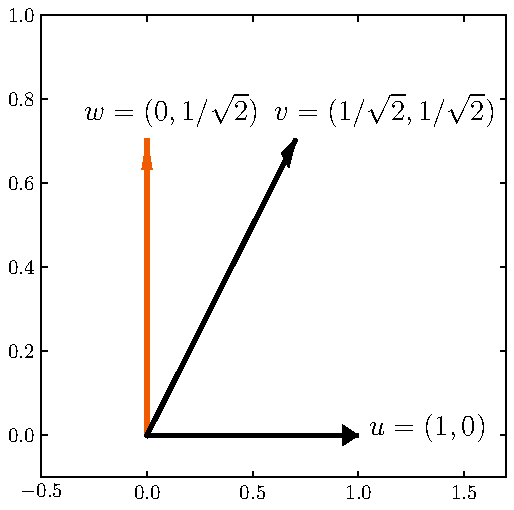
\includegraphics[width=0.6\textwidth]{i5/partiseci.5ex2.eps}
\end{center}

% QUESTION 3
\qs{I.5.3}{Draw any two vectors \(\bm{u}\) and \(\bm{v}\) out from the origin \(\!\left( 0,0 \right) \). Complete two more sides to make a parallelogram with diagonals \(\bm{w} = \bm{u} + \bm{v}\) and \(\bm{z} = \bm{u} - \bm{v}\). Show that \(\bm{w}^{\textsc{T}} \bm{w} + \bm{z}^{\textsc{T}} \bm{z}\) is equal to \(2 \bm{u}^{\textsc{T}} \bm{u} + 2 \bm{v}^{\textsc{T}} \bm{v}\).}

Let \(\bm{u} = \!\left( 1,0 \right) \) and \(\bm{v} = \!\left( 0,1 \right) \). The diagonals are
\begin{align*}
	\bm{w} & = \!\left( 1,0 \right) + \!\left( 0,1 \right) = \!\left( 1,1 \right)  \\
	\bm{z} & = \!\left( 1,0 \right) - \!\left( 0,1 \right) = \!\left( 1, -1 \right)
\end{align*}

Calculating, we find
\begin{align*}
	\bm{w}^{\textsc{T}}\bm{w} + \bm{z}^{\textsc{T}}\bm{z} & = 2 + 2 = 4 \\
	2 \bm{u}^{\textsc{T}}\bm{u} + 2 \bm{v}^{\textsc{T}}\bm{v} & = 2 \!\left( 1 \right) + 2 \!\left( 1 \right) = 4
\end{align*}
Thus equality holds.

\begin{center}
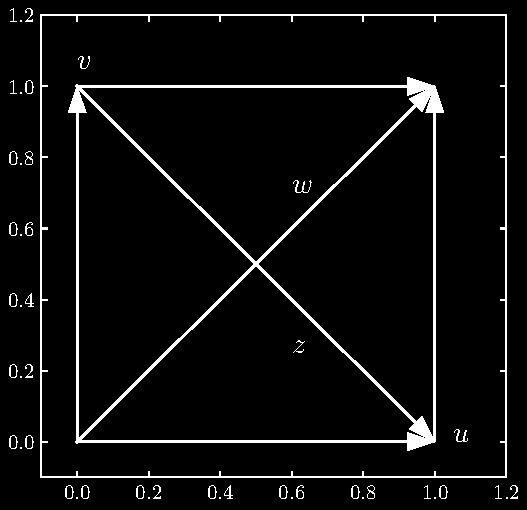
\includegraphics[width=0.6\textwidth]{i5/partiseci.5ex3.eps}
\end{center}

% QUESTION 4
\qs{I.5.4}{Key property of every orthogonal matrix: \(\abs{\abs{Q \bm{x}}}^{2} = \abs{\abs{\bm{x}}}^{2}\) for every vector \(\bm{x}\). More than this, show that \(\!\left( Q \bm{x} \right)^{\textsc{T}} \!\left( Q \bm{y} \right) = \bm{x}^{\textsc{T}} \bm{y}\) for every vector \(\bm{x}\) and \(\bm{y}\). So \textit{lenghts and angles are not changed by} \(Q\). \textbf{Computations with \(\textbf{Q}\) never overflow!}}

We have
\begin{align*}
	\!\left( Q \bm{x} \right)^{\textsc{T}} \!\left( Q \bm{y} \right)  & = \bm{x}^{\textsc{T}}Q^{\textsc{T}} Q \bm{y} \\
	 & = \bm{x}^{\textsc{T}} \bm{y}
\end{align*}

% QUESTION 5
\qs{I.5.5}{If \(Q\) is orthogonal, how do you know that \(Q\) is invertible and \(Q^{-1}\) is also orthogonal? If \(Q_{1}^{\textsc{T}} = Q_{1}^{-1}\) and \(Q_{2}^{\textsc{T}} = Q_{2}^{-1}\), show that \(Q_{1}Q_{2}\) is also an orthogonal matrix.}

By definition of orthogonal, the columns of \(Q\) form an orthonormal basis, meaning they are linearly independent. Hence \(Q\) is invertible. 

Moreover, when \(Q^{-1}Q = I\), we have the columns of \(Q\) times the rows of \(Q^{-1}\) equal to 1, and 0 elsewhere. 

If we had no knowledge of what \(Q^{-1}\) is, we could take a guess at what the rows of \(Q^{-1}\) are. One natural guess is to posit that \textbf{the \(\bm{i}\)-th row of \(\bm{Q^{-1}}\) is the \(\bm{i}\)-th column of \(\bm{Q}\) transposed}. Since by premise \(Q\) is orthogonal, each of its columns times itself is 1 and 0 elsewhere. Notably, by the uniqueness of matrix inversion, \textbf{we can conclude that \(\bm{Q^{-1} = Q^{\textsc{T}}}\)}. Lastly, if the columns of \(Q\) form an orthonormal basis, so must its rows since we also have \(QQ^{-1} = I\). Thus \(Q^{-1} = Q^{\textsc{T}}\) is also orthogonal.

We show that \(Q_{1}Q_{2}\) is orthogonal by
\begin{align*}
	\!\left( Q_{1}Q_{2} \right)^{\textsc{T}} \!\left( Q_{1}Q_{2} \right)  & = Q_{2}^{\textsc{T}}Q_{1}^{\textsc{T}}Q_{1}Q_{2} \\
	 & = Q_{2}^{-1} Q_{1}^{-1}Q_{1}Q_{2} \\ 
	 & = Q_{2}^{-1} Q_{2} \\
	 & = I
\end{align*}

% QUESTION 6
\qs{I.5.6}{A \textbf{permutation matrix} has the same columns as the identity matrix (in some order). \textit{Explain why this permutation matrix and every permutation matrix is orthogonal}:
\[
	P = 
	\begin{bmatrix}
		0 & 1 & 0 & 0 \\
		0 & 0 & 1 & 0 \\
		0 & 0 & 0 & 1 \\
		1 & 0 & 0 & 0 \\
	\end{bmatrix}
	\text{has orthonormal columns so } 
\]
\[
	P^{\textsc{T}}P = \underline{\qquad} \text{ and } P^{-1} = \underline{\qquad}.
\]
When a matrix is symmetric or orthogonal, \textbf{it will have orthogonal eigenvectors}. This is the most important source of orthogonal vectors in applied mathematics.}

One intuition to motivate here is that the transpose of a permutation matrix takes the position of the 1's and \textit{reflects} them over the main diagonal. Therefore, \(PA\) permutes the rows of \(A\), but \(P^{\textsc{T}}PA\) permutes them back to where they were. Therefore, \(P^{\textsc{T}}P\). It immediately follows that \(P^{-1} = P^{\textsc{T}}\). Thus \(P\) is orthogonal. 

\vspace{12pt}

\newpage
% QUESTION 7
\qs{I.5.7}{Four eigenvectors of that matrix \(P\) are \(\bm{x}_{1} = \!\left( 1,1,1,1 \right) \), \(\bm{x}_{2} = \!\left( 1, i, i^{2}, i^{3} \right) \), \(\bm{x}_{3} = \!\left( 1, i^{2}, i^{4}, i^{6} \right) \), and \(\bm{x}_{4} = \!\left( 1, i^{3}, i^{6}, i^{9} \right) \). Multiply \(P\) times each vector to find \(\lambda_{1}\), \(\lambda_{2}\), \(\lambda_{3}\), \(\lambda_{4}\). The eigenvectors are the columns of the 4 by 4 \textbf{Fourier matrix \(\bm{F}\)}.

Show that \(\displaystyle{Q = \frac{F}{2} = \frac{1}{2}
\begin{bmatrix}
	1 & 1 & 1 & 1 \\
	1 & i & -1 & -i \\
	1 & i^{2} & 1 & -1 \\
	1 & i^{3} & -1 & i \\
\end{bmatrix}}\)
\[
	\text{has orthonormal columns: } \bm{\overline{Q}^{\textsc{T}}Q = I}
\]}

Calculate
\[
	P \bm{x}_{1} =
	\begin{bmatrix}
		1 \\
		1 \\
		1 \\
		1 \\
	\end{bmatrix},
	P \bm{x}_{2} =
	\begin{bmatrix}
		i \\
		i^{2} \\
		i^{3} \\
		1 \\
	\end{bmatrix},
	P \bm{x}_{3} =
	\begin{bmatrix}
		i^{2} \\
		i^{4} \\
		i^{6} \\
		1 \\
	\end{bmatrix},
	P \bm{x}_{4} =
	\begin{bmatrix}
		i^{3} \\
		i^{6} \\
		i^{9} \\
		1 \\
	\end{bmatrix}
\]
The eigenvalues are
\[
	\lambda_{1} = 1, \lambda_{2} = i, \lambda_{3} = i^{2}, \lambda_{4} = i^{3}
\]
The Hermitian transpose is
\[
	\overline{Q}^{\textsc{T}} = \frac{1}{2}
	\begin{bmatrix}
		1 & 1 & 1 & 1 \\
		1 & -i & -1 & i \\
		1 & -1 & 1 & -1 \\
		1 & i & -1 & -i \\
	\end{bmatrix}
\]
And so we calculate
\begin{align*}
	\overline{Q}^{\textsc{T}}Q & = \frac{1}{4}
	\begin{bmatrix}
		1 & 1 & 1 & 1 \\
		1 & -i & -1 & i \\
		1 & -1 & 1 & -1 \\
		1 & i & -1 & -i \\
	\end{bmatrix}
	\begin{bmatrix}
		1 & 1 & 1 & 1 \\
		1 & i & -1 & -i \\
		1 & i^{2} & 1 & -1 \\
		1 & i^{3} & -1 & i \\
	\end{bmatrix} \\
	& = \frac{1}{4}
	\begin{bmatrix}
		4 & 0 & 0 & 0 \\
		0 & 4 & 0 & 0 \\
		0 & 0 & 4 & 0 \\
		0 & 0 & 0 & 4 \\
	\end{bmatrix} \\
	& =
	\begin{bmatrix}
		1 & 0 & 0 & 0 \\
		0 & 1 & 0 & 0 \\
		0 & 0 & 1 & 0 \\
		0 & 0 & 0 & 1 \\
	\end{bmatrix}
\end{align*}

\newpage
% QUESTION 8
\qs{I.5.8}{\textbf{Haar wavelets are orthogonal vectors (columns of \(\bm{W}\) using only 1, -1, and 0.}

\(n = 4\)
\[
	W = 
	\begin{bmatrix}
		1 & 1 & 1 & 0 \\
		1 & 1 & -1 & 0 \\
		1 & -1 & 0 & 1 \\
		1 & -1 & 0 & -1 \\
	\end{bmatrix}
\]
\[
\textbf{Find } \bm{W^{\textsc{T}}W} \textbf{ and } \bm{W^{-1}} \textbf{ and the eight Haar wavelets for } \bm{n = 8}.
\]}

Calculate
\[
	W^{\textsc{T}}W = 
	\begin{bmatrix}
		1 & 1 & 1 & 1 \\
		1 & 1 & -1 & -1  \\
		1 & -1 & 0 & 0 \\
		0 & 0 & 1 & 1 \\
	\end{bmatrix}
	\begin{bmatrix}
		1 & 1 & 1 & 0 \\
		1 & 1 & -1 & 0 \\
		1 & -1 & 0 & 1 \\
		1 & -1 & 0 & -1 \\
	\end{bmatrix}
	=
	\begin{bmatrix}
		4 & 0 & 0 & 0 \\
		0 & 4 & 0 & 0 \\
		0 & 0 & 2 & 0 \\
		0 & 0 & 0 & 2 \\
	\end{bmatrix}
\]
\[
	W^{-1} = \frac{1}{4}
	\begin{bmatrix}
		1 & 1 & 1 & 1 \\
		1 & 1 & -1 & -1 \\
		2 & -2 & 0 & 0 \\
		0 & 0 & 2 & -2 \\
	\end{bmatrix}
\]

For \(n = 8\), we have
\[
	W_{8} = 
	\begin{bmatrix}
		1 & 1 & 1 & 0 & 1 & 0 & 0 & 0 \\
		1 & 1 & 1 & 0 & -1 & 0 & 0 & 0 \\
		1 & 1 & -1 & 0 & 0 & 1 & 0 & 0 \\
		1 & 1 & -1 & 0 & 0 & -1 & 0 & 0 \\
		1 & -1 & 0 & 1 & 0 & 0 & 1 & 0 \\
		1 & -1 & 0 & 1 & 0 & 0 & -1 & 0 \\
		1 & -1 & 0 & -1 & 0 & 0 & 0 & 1 \\
		1 & -1 & 0 & -1 & 0 & 0 & 0 & -1 \\
	\end{bmatrix}
\]

\newpage
\subsection{\textsf{I.6 - Eigenvalues and Eigenvectors}}

% QUESTION 1
\qs{I.6.1}{The rotation \(Q =
\begin{bmatrix}
	\cos \theta   & -\sin \theta  \\
	\sin \theta  & \cos \theta  \\
\end{bmatrix}\) has complex eigenvalues \(\lambda = \cos \theta \pm i \sin \theta \):
\[
	Q
	\begin{bmatrix}
		1 \\
		-i \\
	\end{bmatrix}
	=
	\!\left( \cos \theta + i \sin \theta  \right) 
	\begin{bmatrix}
		1 \\
		-i \\
	\end{bmatrix}
	\text{ and }
	Q
	\begin{bmatrix}
		1 \\
		i \\
	\end{bmatrix}
	=
	\!\left( \cos \theta - i \sin \theta  \right) 
	\begin{bmatrix}
		1 \\
		i \\
	\end{bmatrix}.
\]
Check that \(\lambda_{1} + \lambda_{2}\) equals the trace of \(Q\) (sum \(Q_{11} + Q_{22}\) down the diagonal). Check that \(\!\left( \lambda_{1} \right) \!\left( \lambda_{2} \right) \) equals the determinant. Check that those complex eigenvectors are orthogonal, using the complex dot product \(\overline{\bm{x}}_{1} \cdot \bm{x}_{2}\) (not just \(\bm{x}_{1} \cdot \bm{x}_{2}!\)).}

We have \(\lambda_{1} + \lambda_{2} = 2 \cos \theta = \text{tr } Q\). 

Moreover, \(\!\left( \cos \theta + i \sin \theta  \right) \!\left( \cos \theta - i \sin \theta \right) = 1 = \det Q\).

Lastly,
\[
	\overline{\bm{x}}_{1} \cdot \bm{x}_{2} = 1 + i^{2} = 0
\]
Confirming that the complex eigenvectors are orthogonal.

\vspace{12pt}

% QUESTION 2
\qs{I.6.2}{Compute the eigenvalues and eigenvectors of \(A\) and \(A^{-1}\). Check the trace!
\[
	A = 
	\begin{bmatrix}
		0 & 2 \\
		1 & 1 \\
	\end{bmatrix}
	\qquad
	\text{and}
	\qquad
	A^{-1} =
	\begin{bmatrix}
		-1/2 & 1 \\
		1/2 & 0 \\
	\end{bmatrix}.
\]
\(A^{-1}\) has the \underline{\qquad} eigenvectors as \(A\). When \(A\) has eigenvalues \(\lambda_{1}\) and \(\lambda_{2}\), its inverse has eigenvectors \underline{\qquad}.}

Calculate
\[
	\det \!\left( A - \lambda I \right) = -\lambda \!\left( 1 - \lambda  \right) - 2 = \lambda^{2} - \lambda - 2 = 0
\]
which has roots \(\lambda_{1} = -1\), \(\lambda_{2} = 2\). Confirm that \(\!\left( \lambda_{1} \right) \!\left( \lambda_{2} \right) = \!\left( -1 \right) \!\left( 2 \right) = -2 = \det A\) and \(\lambda_{1} + \lambda_{2} = 1 = \text{tr }A\). We derive the eigenvectors from
\[
	\!\left( A - \lambda I \right) \bm{x} = 
	\begin{bmatrix}
		-\lambda  & 2 \\
		1 & 1 - \lambda  \\
	\end{bmatrix}
	\bm{x} = \bm{0}
\]
and find
\[
	\bm{x}_{1} =
	\begin{bmatrix}
		2 \\
		-1 \\
	\end{bmatrix},
	\quad
	\bm{x}_{2} =
	\begin{bmatrix}
		1 \\
		1 \\
	\end{bmatrix}
\]
For \(A^{-1}\), we have
\[
	\det \!\left( A^{-1} - \lambda I \right) = \lambda \!\left(1/2 + \lambda   \right) - 1/2 = \lambda^{2} + \lambda/2 - 1/2 
\]
which has roots \(\lambda_{1} = -1\), \(\lambda_{2} = 1/2\). Confirm that \(\!\left( \lambda_{1} \right) \!\left( \lambda_{2} \right) = \!\left( -1 \right) \!\left( 1/2 \right) = -1/2 = \det A\) and \(\lambda_{1} + \lambda_{2} = -1/2 = \text{tr }A^{-1}\). The eigenvectors are
\[
	\!\left( A^{-1} - \lambda I \right) \bm{x} = 
	\begin{bmatrix}
		-1/2 - \lambda  & 1 \\
		1/2 & -\lambda  \\
	\end{bmatrix}
	\bm{x} = \bm{0}
\]
\[
	\bm{x}_{1} = 
	\begin{bmatrix}
		2 \\
		-1 \\
	\end{bmatrix},
	\quad
	\bm{x}_{2} =
	\begin{bmatrix}
		1 \\
		1 \\
	\end{bmatrix}
\]
The inverse has the same eigenvectors as the original matrix. In the former case, the eigenvalues are of form \(1/\lambda \), as expected.

\vspace{12pt}

% QUESTION 3
\qs{I.6.3}{Find the eigenvalues of \(A\) and \(B\) (easy for triangular matrices) and \(A + B\):
\[
	A = 
	\begin{bmatrix}
		3 & 0 \\
		1 & 1 \\
	\end{bmatrix}
	\text{ and }
	B = 
	\begin{bmatrix}
		1 & 1 \\
		0 & 3 \\
	\end{bmatrix}
	\text{ and }
	A + B =
	\begin{bmatrix}
		4 & 1 \\
		1 & 4 \\
	\end{bmatrix}
\]
Eigenvalues of \(A + B\) (\textit{are equal to})(\textit{are not equal to}) eigenvalues of \(A\) plus eigenvalues of \(B\).}

We have \(\lambda_{A,1} = 3\), \(\lambda_{A,2} = 1\) and \(\lambda_{B,1} = 1\), \(\lambda_{B,2} = 3\). The eigenvalues of \(A + B\) are
\[
	\det \!\left( A + B - \lambda I \right) = \!\left( 4 - \lambda \right)^{2} - 1 = \lambda^{2} - 8 \lambda + 15 = 0 
\]
From which we derive \(\lambda_{1} = 5\), \(\lambda_{2} = 3\). Thus eigenvalues of \(A + B\) are not equal to the sum eigenvalues for \(A\) and \(B\).

\vspace{12pt}

% QUESTION 4
\qs{I.6.4}{Find the eigenvalues of \(A\) and \(B\) and \(AB\) and \(BA\):
\[
	A = 
	\begin{bmatrix}
		1 & 0 \\
		1 & 1 \\
	\end{bmatrix}
	\text{ and }
	B =
	\begin{bmatrix}
		1 & 2 \\
		0 & 1 \\
	\end{bmatrix}
	\text{ and }
	AB = 
	\begin{bmatrix}
		1 & 2 \\
		1 & 3 \\
	\end{bmatrix}
	\text{ and }
	BA = 
	\begin{bmatrix}
		3 & 2 \\
		1 & 1 \\
	\end{bmatrix}
\]
\begin{enumerate}[label=(\alph*)]
	\item Are the eigenvalues of \(AB\) equal to eigenvalues of \(A\) times eigenvalues of \(B\)?
	\item Are the eigenvalues of \(AB\) equal to the eigenvalues of \(BA\)?
\end{enumerate}}

We have
\[
	\lambda_{A,1,2} = 1, 1 \quad \lambda_{B,1,2} = 1, 1 \quad \lambda_{AB, 1, 2} = 2 \pm \sqrt{3} \quad \lambda_{BA, 1, 2} = 2 \pm \sqrt{3}
\]
\par (a) No

(b) Yes

\vspace{12pt}

% QUESTION 5
\qs{I.6.5}{
\begin{enumerate}[label=(\alph*)]
	\item If you know that \(\bm{x}\) is an eigenvector, the way to find \(\lambda \) is to \underline{\qquad}.
	\item If you know that \(\lambda \) is an eigenvalue, the way to find \(\bm{x}\) is to \underline{\qquad}.
\end{enumerate}}

(a) Multiply \(A \bm{x}\) and find the scaling factor on \(\bm{x}\). That is \(\lambda \).

\par (b) Solve \(\!\left( A - \lambda I \right) \bm{x} = \bm{0}\).

\vspace{12pt}

% QUESTION 6
\qs{I.6.6}{Find the eigenvalues and eigenvectors for both of these Markov matrices \(A\) and \(A^{\infty}\). Explain from those answers why \(A^{100}\) is close to \(A^{\infty}\):
\[
	A =
	\begin{bmatrix}
		.6 & .2 \\
		.4 & .8 \\
	\end{bmatrix}
	\quad
	\text{and}
	\quad
	A^{\infty} =
	\begin{bmatrix}
		1/3 & 1/3 \\
		2/3 & 2/3 \\
	\end{bmatrix}
\]}

We have
\[
	\lambda_{A,1,2} = 1, 0.4 \qquad \lambda_{A^{\infty}, 1, 2} = 1, 0
\]
with eigenvectors
\[
	\bm{x}_{A,1,2} = \bm{x}_{A^{\infty},1,2} = 
	\begin{bmatrix}
		1/2 \\
		1 \\
	\end{bmatrix},
	\begin{bmatrix}
		-1 \\
		1 \\
	\end{bmatrix}
\]
For any vector \(\bm{v}\), we have
\[
	A^{k} \bm{v} = c_{1} \!\left( 1 \right)^{k} \bm{x}_{1} + c_{2} \!\left( 0.4 \right)^{k} \bm{x}_{2}
\]
As \(k \rightarrow \infty\), \(\!\left( 0.4 \right)^{k} \rightarrow 0\). When \(k = 100\), \(\!\left( 0.4 \right)^{k}\) is effectively zero. Since the eigenvectors are the same, and the eigenvalues \textit{essentially} the same, it must be that \(A^{100}\) asymptotically approaches \(A^{\infty}\).

\vspace{12pt}

% QUESTION 7
\qs{I.6.7}{\textbf{The determinant of \(A\) equals the product} \(\lambda_{1}\lambda_{2}\cdots \lambda_{n}\). Start with the polynomial \(\det \!\left( A - \lambda I \right) \) separated into its \(n\) factors (always possible). Then set \(\lambda = 0\):
\[
	\det \!\left( A - \lambda I \right) = \!\left( \lambda_{1} - \lambda \right) \!\left( \lambda_{2} - \lambda  \right) \cdots \!\left( \lambda_{n} - \lambda  \right) \text{ so } \det A = \underline{\qquad}.
\]
Check this rule in Example 1 where the Markov matrix has \(\lambda = 1\) and \(\frac{1}{2}\).}

In general
\[
	\det A = \prod_{k=1}^{n} \lambda_{k} 
\]
In the case of the Markov matrix, we have
\[
	A =
	\begin{bmatrix}
		0.8 & 0.3 \\
		0.2 & 0.7 \\
	\end{bmatrix},
	\quad
	\det A = 0.5 = \lambda_{1}\lambda_{2}
\]
\newpage
% QUESTION 8
\qs{I.6.8}{The sum of the diagonal entries (the \textit{trace}) equals the sum of the eigenvalues:
\[
	A = 
	\begin{bmatrix}
		a & b \\
		c & d \\
	\end{bmatrix}
	\text{ has }
	\det \!\left( A - \lambda I \right) = \lambda^{2} - \!\left( a + d \right)\lambda + ad - bc = 0
\]
The quadratic formula gives the eigenvalues \(\lambda = \!\left( a + d + \sqrt{\quad} \right)/2 \) and \(\lambda = \underline{\qquad}\). Their sum is \(\underline{\qquad}\). If \(A\) has \(\lambda_{1} = 3\) and \(\lambda_{2} = 4\) then \(\det \!\left( A - \lambda I \right) = \underline{\qquad}\).}

The discriminant is
\[
	\!\left( a + d \right)^{2} - 4 \!\left( ad - bc \right) 
\]
and the other eigenvalue is
\[
	\lambda = \frac{a + d - \sqrt{\!\left( a + d \right)^{2} - 4 \!\left( ad - bc \right) }}{2} 
\]
The sum of the eigenvalues is
\[
	\lambda_{1} + \lambda_{2} = a + d
\]
With eigenvalues \(\lambda_{1} = 3\), \(\lambda_{2} = 4\), we have
\[
	\det \!\left( A - \lambda I \right) = \!\left( 3 - \lambda  \right) \!\left( 4 - \lambda  \right) 
\]
% QUESTION 9
\qs{I.6.9}{If \(A\) has \(\lambda_{1} = 4\) and \(\lambda_{2} = 5\) then \(\det \!\left( A - \lambda I \right) = \!\left( \lambda - 4 \right) \!\left( \lambda - 5 \right) = \lambda^{2} - 9 \lambda + 20\). Find three matrices that have trace \(a + d = 9\) and determinant 20 and \(\lambda = 4,5\).}

\[
	A =
	\begin{bmatrix}
		4 & 0 \\
		0 & 5 \\
	\end{bmatrix}
	\quad
	B =
	\begin{bmatrix}
		5 & 0 \\
		0 & 4 \\
	\end{bmatrix}
	\quad
	C =
	\begin{bmatrix}
		4 & 1 \\
		0 & 5 \\
	\end{bmatrix}
\]

% QUESTION 10
\qs{I.6.10}{Choose the last rows of \(A\) and \(C\) to give eigenvalues 4, 7, and 1, 2, 3:
\[
	\textbf{Companion Matrices} \qquad A =
	\begin{bmatrix}
		0 & 1 \\
		* & * \\
	\end{bmatrix}
	\quad
	C =
	\begin{bmatrix}
		0 & 1 & 0 \\
		0 & 0 & 1 \\
		* & * & * \\
	\end{bmatrix}
\]}

Given the matrix
\[
	A =
	\begin{bmatrix}
		0 & 1 \\
		a & b \\
	\end{bmatrix}
\]
We have characteristic polynomial
\[
	\det \!\left( A - \lambda I \right) = -\lambda \!\left( b - \lambda  \right) - a = \lambda^{2} - b \lambda - a  = 0
\]
which itself must be equal to
\[
	\!\left( 4 - \lambda  \right) \!\left( 7 - \lambda  \right) = \lambda^{2} - 11 \lambda + 28 = 0
\]
allowing us to conclude that \(a = -28\) and \(b = 11\).

In the case of \(C\), let \(a\), \(b\), \(c\) be the last row. We have characteristic polynomial
\[
	\det \!\left( C - \lambda I \right) = a + b \lambda + c \lambda^{2} - \lambda^{3}
\]
which is equal to
\[
	\!\left( 1 - \lambda  \right) \!\left( 2 - \lambda  \right) \!\left( 3 - \lambda  \right) = 6 - 11 \lambda + 6 \lambda^{2} - \lambda^{3}
\]
Thus we have \(a = 6\), \(b = -11\), \(c = 6\).

\vspace{12pt}

% QUESTION 11
\qs{I.6.11}{\textbf{\textit{The eigenvalues of \(\bm{A}\) equal the eigenvalues of}} \(\bm{A}^{\textsc{T}}\). This is because \(\det \!\left( A - \lambda I \right) \) equals \(\det \!\left( A^{\textsc{T}} - \lambda I \right) \). That is true because \underline{\qquad}. Show by an example that the eigenvectors of \(A\) and \(A^{\textsc{T}}\) are \textit{not} the same.}

Determinants are invariant under transpose, so the determinants of \(A - \lambda I\) and \(A^{\textsc{T}} - \lambda I\) are equal.

Consider the matrix
\[
	A = 
	\begin{bmatrix}
		1 & 1 \\
		0 & 1 \\
	\end{bmatrix}
\]
Its eigenvalues are \(\lambda_{1,2} = 1\) (repeated), but its one eigenvector is \(\bm{x} = 
\begin{bmatrix}
	1 \\
	0 \\
\end{bmatrix}
\) . However, \(A^{\textsc{T}}\) still has eigenvalues \(\lambda_{1,2} = 1\), while its eigenvector is \(
\bm{x} =
\begin{bmatrix}
	0 \\
	1 \\
\end{bmatrix}
\).

% QUESTION 12
\qs{I.6.12}{This matrix is singular with rank one. Find three \(\lambda\)'s and three eigenvectors:
\[
	A =
	\begin{bmatrix}
		1 \\
		2 \\
		1 \\
	\end{bmatrix}
	\begin{bmatrix}
		2 & 1 & 2 \\
	\end{bmatrix} =
	\begin{bmatrix}
		2 & 1 & 2 \\
		4 & 2 & 4 \\
		2 & 1 & 2 \\
	\end{bmatrix}
\]}

Because the matrix is singular, we should expect at least one eigenvalue equal to zero. Let's see what happens when we derive the characteristic polynomial:
\begin{align*}
	\det \!\left( A - \lambda I \right) & = \!\left( 2 - \lambda  \right) \!\left[ \!\left( 2 - \lambda  \right)^{2} - 4 \right] - \!\left[ 4 \!\left( 2 - \lambda  \right) - 8 \right] + 2 \!\left[ 4 - 2 \!\left( 2 - \lambda  \right)  \right] \\
			& = \!\left( 2 - \lambda  \right)^{3} - 12 \!\left( 2 - \lambda  \right) + 16 \\
			& = \lambda^{2} \!\left( 6 - \lambda  \right)  \\
			& \implies \lambda_{1,2} = 0, \lambda_{3} = 6 
\end{align*}

In particular, for real symmetric matrices, the multiplicity of zero eigenvalues equals the nullity of the matrix.

Three eigenvectors are:
\[
	x_{1} =
	\begin{bmatrix}
		1 \\
		-2 \\
		0 \\
	\end{bmatrix}, \quad
	x_{2} = 
	\begin{bmatrix}
		0 \\
		1 \\
		-2 \\
	\end{bmatrix}, \quad
	x_{3} =
	\begin{bmatrix}
		1 \\
		2 \\
		1 \\
	\end{bmatrix}
\]
which correspond to \(\lambda_{1,2,3}\) respectively.

\vspace{12pt}

% QUESTION 13
\qs{I.6.13}{Suppose \(A\) and \(B\) have the same eigenvalues \(\lambda_{1}, \ldots, \lambda_{n}\) with the same independent eigenvectors \(\bm{x}_{1}, \ldots, \bm{x}_{n}\). Then \(A = B\). \textit{Reason}: Any vector \(\bm{x}\) is a combination \(c_{1}\bm{x}_{1} + \cdots + c_{n}\bm{x}_{n}\). What is \(A \bm{x}\)? What is \(B \bm{x}\)?}

Take any arbitrary \(\bm{x}\). Then we have
\begin{align*}
	A \bm{x} & = A \!\left( c_{1}\bm{x}_{1} + \cdots + c_{n} \bm{x}_{n} \right)  \\
	 & = c_{1} A \bm{x}_{1} + \cdots + c_{n} A \bm{x}_{n} \\ 
	 & = c_{1} \lambda_{1} + \cdots + c_{n} \lambda_{n} \\
	B \bm{x} & = B \!\left( c_{1} \bm{x}_{1} + \cdots + c_{n} \bm{x}_{n} \right) \\
		 & = c_{1} B \bm{x}_{1} + \cdots + c_{n} B \bm{x}_{n} \\
		 & = c_{1} \lambda_{1} + \cdots + c_{n} \lambda_{n}
\end{align*}

Thus for any \(\bm{x}\), \(A \bm{x} = B \bm{x}\). Ergo, we must have \(A = B\).

\vspace{12pt}

% QUESTION 14
\qs{I.6.14}{Suppose \(A\) has eigenvalues \(0\), \(3\), \(5\) with independent eigenvectors \(\bm{u}, \bm{v}, \bm{w}\).
\begin{enumerate}[label=(\alph*)]
	\item Give a basis for the nullspace and a basis for the column space.
	\item Find a particular solution to \(A \bm{x} = \bm{v} + \bm{w}\). Find all solutions.
	\item \(A \bm{x} = \bm{u}\) has no solution. If it did then \underline{\qquad} would be in the column space.
\end{enumerate}}

Firstly, this arrangement enables us to write the following matrix equations:
\begin{align*}
	A \bm{u} & = \bm{0} \\
	A \bm{v} & = 3 \bm{v} \\ 
	A \bm{w} & = 5 \bm{w}
\end{align*}

(a) One basis for \(\textbf{N} \!\left( A \right) \) is
\[
	\bm{u}
\]
and a basis for \(\textbf{C} \!\left( A \right) \) is
\[
	\bm{v}, \bm{w}
\]
(b) A particular solution is \(\bm{x} = \displaystyle{\frac{1}{3}} \bm{v} + \frac{1}{5} \bm{w}\), which yields
\[
	A \!\left( \frac{1}{3} \bm{v} + \frac{1}{5}\bm{w} \right) = \frac{1}{3} A \bm{v} + \frac{1}{5} A \bm{w} = \bm{v} + \bm{w}
\]
In general, for any scalar \(c\), we have general solution \(\bm{x} = \frac{1}{3} \bm{v} + \frac{1}{5} \bm{w} + c \bm{u}\):
\[
	A \!\left( \frac{1}{3} \bm{v} + \frac{1}{5} \bm{w} + c \bm{u} \right) = \bm{v} + \bm{w}
\]
(c) If a solution to \(A \bm{x} = \bm{u}\) existed, then \(\bm{u}\) would be in the column space.

\vspace{12pt}

% QUESTION 15
\qs{I.6.15}{
\begin{enumerate}[label=(\alph*)]
	\item Factor these two matrices into \(A = X \Lambda X^{-1}\):
		\[
			A = 
			\begin{bmatrix}
				1 & 2 \\
				0 & 3 \\
			\end{bmatrix} \quad
			\text{and} \quad
			A = 
			\begin{bmatrix}
				1 & 1 \\
				3 & 3 \\
			\end{bmatrix}
		\]
	\item If \(A = X \Lambda X^{-1}\) then \(A^{3} = \!\left( \quad \right) \!\left( \quad \right) \!\left( \quad \right)  \) and \(A^{-1}= \!\left( \quad \right) \!\left( \quad \right) \!\left( \quad \right) \).
\end{enumerate}}

(a) 
\[
	A = 
	\begin{bmatrix}
		1 & 2 \\
		0 & 3 \\
	\end{bmatrix} =
	\begin{bmatrix}
		1 & 1 \\
		0 & 1 \\
	\end{bmatrix}
	\begin{bmatrix}
		1 & 0 \\
		0 & 3 \\
	\end{bmatrix}
	\begin{bmatrix}
		1 & -1 \\
		0 & 1 \\
	\end{bmatrix}
\]
\[
	A = 
	\begin{bmatrix}
		1 & 1 \\
		3 & 3 \\
	\end{bmatrix}
	= \frac{1}{4}
	\begin{bmatrix}
		1 & 1 \\
		-1 & 3 \\
	\end{bmatrix}
	\begin{bmatrix}
		0 & 0 \\
		0 & 4 \\
	\end{bmatrix}
	\begin{bmatrix}
		3 & -1 \\
		1 & 1 \\
	\end{bmatrix}
\]

(b) We have
\[
	A^{3} = X \Lambda^{3} X^{-1} \quad \text{and} \quad A^{-1} = X \Lambda^{-1} X^{-1}
\]

% QUESTION 16
\qs{I.6.16}{Suppose \(A = X \Lambda X^{-1}\). What is the eigenvalue matrix for \(A + 2I\)? What is the eigenvector matrix? Check that \(A + 2I = \!\left( \quad \right) \!\left( \quad \right) \!\left( \quad \right)^{-1}\).}

We have
\[
	A + 2I = X \!\left( \Lambda + 2I \right) X^{-1}
\]
We can ascertain this result by demonstrating that
\[
	X \!\left( \Lambda + 2I \right) X^{-1} = X \Lambda X^{-1} + 2 XX^{-1} = A + 2I
\]
% QUESTION 17
\qs{I.6.17}{True or false: If the columns of \(X\) (eigenvectors of \(A\)) are linearly independent, then

\begin{enumerate}[label=(\alph*)]
	\item \(A\) is invertible
	\item \(A\) is diagonalizable
	\item \(X\) is invertible
	\item \(X\) is diagonalizable
\end{enumerate}}

(a) \textbf{False}. Refer to the matrix in exercise 12.

(b) \textbf{True}. That \(X\) exists implies the diagonalizability of \(A\).

(c) \textbf{True}. Linear independence of the columns implies invertibility.

(d) \textbf{Unknown}. Depends on what \(X\) is.

\vspace{12pt}

% QUESTION 18
\qs{I.6.18}{Write down the most general matrix that has eigenvectors \(
\begin{bmatrix}
	\bm{1} \\
	\bm{1} \\
\end{bmatrix}\) and 
\(\begin{bmatrix}
	\bm{1} \\
	\bm{-1} \\
\end{bmatrix}\).}

This matrix is of form
\[
	A = \frac{1}{2}
	\begin{bmatrix}
		1 & 1 \\
		1 & -1 \\
	\end{bmatrix}
	\begin{bmatrix}
		\lambda_{1} & 0 \\
		0 & \lambda_{2} \\
	\end{bmatrix}
	\begin{bmatrix}
		1 & 1 \\
		1 & -1 \\
	\end{bmatrix}
	=
	\begin{bmatrix}
		\lambda_{1} + \lambda_{2} & \lambda_{1} - \lambda_{2} \\
		\lambda_{1} - \lambda_{2} & \lambda_{1} + \lambda_{2} \\
	\end{bmatrix} =
	\begin{bmatrix}
		a & b \\
		b & a \\
	\end{bmatrix}
\]

% QUESTION 19
\qs{I.6.19}{True or false: If the eigenvalues of \(A\) are \(2\), \(2\), \(5\) then the matrix is certainly
\begin{enumerate}[label=(\alph*)]
	\item invertible
	\item diagonalizable
	\item not diagonalizable
\end{enumerate}}

The matrix is certainly invertible, as we have non-zero eigenvalues. The diagonalizability of the matrix is contingent on whether the geometric multiplicity (number of independent eigenvectors) equals the arithmetic multiplicity (number of repeating eigenvalues) of 2.

\vspace{12pt}

% QUESTION 20
\qs{I.6.20}{True or false: If the only eigenvectors of \(A\) are multiples of \(\!\left( 1,4 \right) \) then \(A\) has
\begin{enumerate}[label=(\alph*)]
	\item no inverse
	\item a repeated eigenvalue
	\item no diagonalization \(X \Lambda X^{-1}\).
\end{enumerate}}

(a) \textbf{Impossible to say}. This is contingent on whether there is a zero eigenvalue.

(b) \textbf{True}. The existence of only a single eigenvector implies that the geometric multiplicity is less than the arithmetic multiplicity; ergo, we have a repeated eigenvalue.

(c) \textbf{True}. Since \(X\) is singular, there cannot be a diagonalization \(X \Lambda X^{-1}\).

\vspace{12pt}

% QUESTION 21
\qs{I.6.21}{\(A^{k} = X \Lambda^{k} X^{-1}\) approaches the zero matrix as \(k \rightarrow \infty\) if and only if every \(\lambda \) has absolute value less than \underline{\qquad}. Which of these matrices has \(A^{k} \rightarrow 0\)?
\[
	A_{1} = 
	\begin{bmatrix}
		.6 & .9 \\
		.4 & .1 \\
	\end{bmatrix} \quad
	\text{and} \quad
	A_{2} = 
	\begin{bmatrix}
		.6 & .9 \\
		.1 & .6 \\
	\end{bmatrix}
\]}

\(A^{k} \rightarrow 0\) if and only if every \(\abs{\lambda } < 0\). Here, \(A_{1}\) has eigenvalues \(\lambda_{1,2} = 1, -0.3\) and \(A_{2}\) has eigenvalues \(\lambda_{1,2} = 0.9, 0.3\). Thus only \(A_{2}^{k} \rightarrow 0\) as \(k \rightarrow \infty\).

\vspace{12pt}

% QUESTION 22
\qs{I.6.22}{Diagonalize \(A\) and compute \(X \Lambda X^{-1}\) to prove this formula for \(A^{k}\):
\[
	A = 
	\begin{bmatrix}
		2 & -1 \\
		-1 & 2 \\
	\end{bmatrix}
	\quad
	\text{and}
	\quad
	A^{k} = \frac{1}{2}
	\begin{bmatrix}
		1 + 3^{k} & 1 - 3^{k} \\
		1 - 3^{k} & 1 + 3^{k} \\
	\end{bmatrix}
\]}

We have eigenvalues \(\lambda_{1,2} = 3, 1\) and eigenvectors \(\bm{x}_{1} = 
\begin{bmatrix}
	1 \\
	-1 \\
\end{bmatrix}\) and \(\bm{x}_{2} = 
\begin{bmatrix}
	1 \\
	1 \\
\end{bmatrix}\). Then we can write
\[
	A^{k} = \frac{1}{2}
	\begin{bmatrix}
		1 & 1 \\
		-1 & 1 \\
	\end{bmatrix}
	\begin{bmatrix}
		3^{k} & 0 \\
		0 & 1^{k} \\
	\end{bmatrix}
	\begin{bmatrix}
		1 & -1 \\
		1 & 1 \\
	\end{bmatrix} = \frac{1}{2}
	\begin{bmatrix}
		1 + 3^{k} & 1 - 3^{k} \\
		1 - 3^{k} & 1 + 3^{k} \\
	\end{bmatrix}
\]

% QUESTION 23
\qs{I.6.23}{The eigenvalues of \(A\) are \(1\) and \(9\), and the eigenvalues of \(B\) are \(-1\) and \(9\):
\[
	A = 
	\begin{bmatrix}
		5 & 4 \\
		4 & 5 \\
	\end{bmatrix}
	\quad
	\text{and}
	\quad
	B = 
	\begin{bmatrix}
		4 & 5 \\
		5 & 4 \\
	\end{bmatrix}
\]
Find a matrix square root of \(A\) from \(R = X \sqrt{\Lambda} X^{-1}\). Why is there no real matrix square root of \(B\)?}

\(A\) has eigenvectors \(\bm{x}_{1} = 
\begin{bmatrix}
	1 \\
	-1 \\
\end{bmatrix}\) and \(\bm{x}_{2} = 
\begin{bmatrix}
	1 \\
	1 \\
\end{bmatrix}\). We have matrix square root
\[
	A^{1/2} = \frac{1}{2}
	\begin{bmatrix}
		1 & 1 \\
		-1 & 1 \\
	\end{bmatrix}
	\begin{bmatrix}
		1 & 0 \\
		0 & 3 \\
	\end{bmatrix}
	\begin{bmatrix}
		1 & -1 \\
		1 & 1 \\
	\end{bmatrix} =
	\begin{bmatrix}
		2 & 1 \\
		1 & 2 \\
	\end{bmatrix}
\]

For \(B\), we have a negative eigenvalue, for which it is impossible to take a real square root.

\vspace{12pt}

% QUESTION 24
\qs{I.6.24}{Suppose the same \(X\) diagonalizes both \(A\) and \(B\). They have the \textit{same eigenvectors} in \(A = X \Lambda_{1} X^{-1}\) and \(B = X \Lambda_{2} X^{-1}\). Prove that \(AB = BA\).}

We have
\begin{align*}
	AB & = \!\left( X \Lambda_{1} X^{-1} \right) \!\left( X \Lambda_{2} X^{-1} \right) = X \Lambda_{1} \Lambda_{2} X^{-1}  \\
	   & = X \Lambda_{2} \Lambda_{1} X^{-1} = \!\left( X \Lambda_{2} X^{-1} \right) \!\left( X \Lambda_{1} X^{-1} \right) = BA
\end{align*}

where the equality on the second line is permissible because the multiplication of diagonal matrices commute.

\vspace{12pt}

\vspace{12pt}

% QUESTION 25
\qs{I.6.25}{The transpose of \(A = X \Lambda X^{-1}\) is \(A^{\textsc{T}} = \!\left( X^{-1} \right)^{\textsc{T}} \Lambda X^{\textsc{T}}\). The eigenvectors in \(A^{\textsc{T}} \bm{y} = \lambda \bm{y}\) are the columns of that matrix \(\!\left( X^{-1} \right)^{\textsc{T}}\). They are often called \textbf{\textit{left eigenvectors of \(\bm{A}\)}}, because \(\bm{y}^{\textsc{T}} A = \lambda \bm{y}^{\textsc{T}}\). How do you multiply matrices to find this formula for \(A\)?

\vspace{12pt}

\boxed{\textbf{Sum of rank-1 matrices} \quad A = X \Lambda X^{-1} = \lambda_{1} \bm{x}_{1} \bm{y}_{1}^{\textsc{T}} + \cdots + \lambda_{n} \bm{x}_{n} \bm{y}_{n}^{\textsc{T}}}
}

By the decomposition into the sum of rank-1 matrices, we need only multiply the columns of \(X\) and the rows of \(X^{-1}\). The product of the \(n\)-th column and row is scaled by the \(n\)-th eigenvalue in \(\Lambda\), \(\lambda_{n}\).

\vspace{12pt}

% QUESTION 26
\qs{I.6.26}{\textbf{When is a matrix \(\bm{A}\) similar to its eigenvalue matrix \(\bm{\Lambda}\)?}
\(A\) and \(\Lambda\) always have the same eigenvalues. But similarity requires a matrix \(B\) with \(A = B \Lambda B^{-1}\). Then \(B\) is the \underline{\qquad} matrix and \(A\) must have \(n\) independent \underline{\qquad}.
}

We must have \(B\) as the \(X\) matrix of \(n\) independent eigenvectors.

\newpage
\subsection{\textsf{I.7 - Symmetric Positive Definite Matrices}}

% QUESTION 1
\qs{I.7.1}{Suppose \(S^{\textsc{T}} = S\) and \(S \bm{x} = \lambda \bm{x}\) and \(S \bm{y} = \alpha \bm{y}\) are all real. Show that
\[
	\bm{y}^{\textsc{T}} S \bm{x} = \lambda \bm{y}^{\textsc{T}} \bm{x} \quad \text{and} \quad \bm{x}^{\textsc{T}} S \bm{y} = \alpha \bm{x}^{\textsc{T}} \bm{y} \quad \text{and} \quad \bm{y}^{\textsc{T}} S \bm{x} = \bm{x}^{\textsc{T}} S \bm{y}.
\]
Show that \(\bm{y}^{\textsc{T}}\bm{x}\) must be zero if \(\lambda \neq \alpha \): \textbf{orthogonal eigenvectors}.}

For the first identity, left-muliply \(S \bm{x} = \lambda \bm{x}\) by \(\bm{y}^{\textsc{T}}\). For the second, left-multiply \(S \bm{y} = \alpha \bm{y}\) by \(\bm{x}^{\textsc{T}}\). Lastly, suppose that \(\lambda  = \alpha \). Then \(\bm{y}^{\textsc{T}}S \bm{x} = \bm{x}^{\textsc{T}} S \bm{y}\) since \(\bm{y}^{\textsc{T}}\bm{x} = \bm{x}^{\textsc{T}}\bm{y}\). However, suppose that \(\lambda \neq \alpha \). By the Spectral Theorem, \(\bm{x}\) and \(\bm{y}\) are orthogonal. Thus the equality for the third identity still holds (both equal to zero) and \(\bm{y}^{\textsc{T}}\bm{x} = 0\).

\vspace{12pt}

% QUESTION 2
\qs{I.7.2}{Which of \(S_{1}\), \(S_{2}\), \(S_{3}\), \(S_{4}\) has two positive eigenvalues? Use a test, don't compute the \(\lambda \)'s. Also find an \(\bm{x}\) so that \(\bm{x}^{\textsc{T}}S_{1}\bm{x} < 0\), so \(S_{1}\) is not positive definite.
\[
	S_{1} =
	\begin{bmatrix}
		5 & 6 \\
		6 & 7 \\
	\end{bmatrix}
	\quad
	S_{2} = 
	\begin{bmatrix}
		-1 & -2 \\
		-2 & -5 \\
	\end{bmatrix}
	\quad
	S_{3} =
	\begin{bmatrix}
		1 & 10 \\
		10 & 100 \\
	\end{bmatrix}
	\quad
	S_{4} =
	\begin{bmatrix}
		1 & 10 \\
		10 & 101 \\
	\end{bmatrix}
\]}

\textbf{Not} \(S_{1}\), \(\det S_{1} = -1\). Consider \(\bm{x} = 
\begin{bmatrix}
	6 \\
	-5 \\
\end{bmatrix}\):
\[
	\bm{x}^{\textsc{T}}S_{1}\bm{x} =
	\begin{bmatrix}
		6 & -5 \\
	\end{bmatrix}
	\begin{bmatrix}
		5 & 6 \\
		6 & 7 \\
	\end{bmatrix}
	\begin{bmatrix}
		6 \\
		-5 \\
	\end{bmatrix}
	= -5
\]

\textbf{Not} \(S_{2}\), leading determinant \(D_{1} = -1\).

\textbf{Not} \(S_{3}\), \(\text{rank}\!\left( S_{3} \right) = 1\) so pivots are not all zero.

\textbf{Yes} \(S_{4}\), consider \(\bm{x}^{\textsc{T}}S_{4}\bm{x}\):
\[
	\bm{x}^{\textsc{T}}S_{4}\bm{x} = x^{2}_{1} + 20x_{1}x_{2} + 101x^{2}_{2} = \!\left( x_{1} + 10x_{2} \right)^{2} + x^{2}_{2}
\]
which is a sum of squares, so it is strictly positive for non-zero \(\bm{x}\). Ergo \(S_{4}\) is positive definite and has two positive eigenvalues.

\vspace{12pt}

% QUESTION 3
\qs{I.7.3}{For which numbers \(b\) and \(c\) are these matrices positive definite?
\[
	S = 
	\begin{bmatrix}
		1 & b \\
		b & 9 \\
	\end{bmatrix}
	\quad
	S = 
	\begin{bmatrix}
		2 & 4 \\
		4 & c \\
	\end{bmatrix}
	\quad
	S = 
	\begin{bmatrix}
		c & b \\
		b & c \\
	\end{bmatrix}
\]
With the pivots in \(D\) and multiplier in \(L\), factor each \(S\) into \(LDL^{\textsc{T}}\).}

First: we must have \(\det S = 9 - b^{2} > 0\), so \(b < 3\).
\[
	S = 
	\begin{bmatrix}
		1 & b \\
		b & 9 \\
	\end{bmatrix}
	=
	\begin{bmatrix}
		1 & 0 \\
		b & 1 \\
	\end{bmatrix}
	\begin{bmatrix}
		1 & 0 \\
		0 & 9 - b^{2} \\
	f,at\end{bmatrix}
	\begin{bmatrix}
		1 & b \\
		0 & 1 \\
	\end{bmatrix}
\]
Second: we must have \(\det S = 2c - 16 > 0\), so \(c > 8\).
\[
	S = 
	\begin{bmatrix}
		2 & 4 \\
		4 & c \\
	\end{bmatrix}
	=
	\begin{bmatrix}
		1 & 0 \\
		2 & 1 \\
	\end{bmatrix}
	\begin{bmatrix}
		2 & 0 \\
		0 & c - 8 \\
	\end{bmatrix}
	\begin{bmatrix}
		1 & 2 \\
		0 & 1 \\
	\end{bmatrix}
\]

Third: we must have \(c > 0\) and \(\det S = c^{2} - b^{2} > 0\), so we must have \(c > \abs{b}\).
\[
	S =
	\begin{bmatrix}
		c & b \\
		b & c \\
	\end{bmatrix}
	=
	\begin{bmatrix}
		1 & 0 \\
		\displaystyle{\frac{b}{c}} & 1 \\
	\end{bmatrix}
	\begin{bmatrix}
		c & 0 \\
		0 & \displaystyle{\frac{c^{2} - b^{2}}{c}} \\
	\end{bmatrix}
	\begin{bmatrix}
		1 & \displaystyle{\frac{b}{c}} \\
		0 & 1 \\
	\end{bmatrix}
\]

% QUESTION 4
\qs{I.7.4}{Here is a quick "proof" that the eigenvalues of every real matrix \(A\) are real:
\[
	\textbf{False proof} \quad A \bm{x} = \lambda \bm{x} \text{ gives } \bm{x}^{\textsc{T}} A \bm{x} = \lambda \bm{x}^{\textsc{T}}\bm{x}  \text{ so } \lambda = \frac{\bm{x}^{\textsc{T}}A \bm{x}}{\bm{x}^{\textsc{T}}\bm{x}} = \frac{\text{real}}{\text{real}}
\]}

The error is in assuming \(\bm{x}^{\textsc{T}}\bm{x} = 0\). Consider the example of \(A = 
\begin{bmatrix}
	0 & -1 \\
	1 & 0 \\
\end{bmatrix}\), \(\lambda = i\), and \(\bm{x} = \!\left( i,1 \right) \):
\[
	\bm{x}^{\textsc{T}}A \bm{x} =
	\begin{bmatrix}
		i & 1 \\
	\end{bmatrix}
	\begin{bmatrix}
		0 & -1 \\
		1 & 0 \\
	\end{bmatrix}
	\begin{bmatrix}
		i \\
		-1 \\
	\end{bmatrix}
	=
	0 = \lambda \bm{x}^{\textsc{T}}\bm{x}
\]
Another erroneous assumption is also in taking eigenvectors to be real a priori, which they need not be.

% QUESTION 5
\qs{I.7.5}{Write \(S\) and \(B\) in the form \(\lambda_{1} \bm{x}_{1} \bm{x}_{1}^{\textsc{T}} + \lambda_{2} \bm{x}_{2}\bm{x}_{2}^{\textsc{T}}\) of the spectral theorem \(Q \Lambda Q^{\textsc{T}}\):
\[
	S = 
	\begin{bmatrix}
		3 & 1 \\
		1 & 3 \\
	\end{bmatrix}
	\quad
	B =
	\begin{bmatrix}
		9 & 12 \\
		12 & 16 \\
	\end{bmatrix}
	\quad
	\text{(keep } \abs{\abs{\bm{x}_{1}}} = \abs{\abs{\bm{x}_{2}}} = 1).
\]}
\[
	S = 2
	\begin{bmatrix}
		1/\sqrt{2} \\
		-1/\sqrt{2} \\
	\end{bmatrix}
	\begin{bmatrix}
		1/\sqrt{2} & -1/\sqrt{2} \\
	\end{bmatrix}
	+
	4
	\begin{bmatrix}
		1/\sqrt{2} \\
		1/\sqrt{2} \\
	\end{bmatrix}
	\begin{bmatrix}
		1/\sqrt{2} & 1/\sqrt{2} \\
	\end{bmatrix}
\]

% QUESTION 6
\qs{I.7.6}{(Recommended) This matrix \(M\) is antisymmetric and also \underline{\qquad}. Then all its eigenvalues are pure imaginary and they also have \(\abs{\lambda} = 1\). (\(\abs{\abs{M \bm{x}}} = \abs{\abs{\bm{x}}}\) for every \(\bm{x}\) so \(\abs{\abs{\lambda \bm{x}}} = \abs{\abs{\bm{x}}}\) for eigenvectors.) Find all four eigenvalues from the trace of \(M\):
\[
	M = \frac{1}{\sqrt{3}}
	\begin{bmatrix}
		0 & 1 & 1 & 1 \\
		-1 & 0 & -1 & 1 \\
		-1 & 1 & 0 & -1 \\
		-1 & -1 & 1 & 0 \\
	\end{bmatrix}
	\quad
	\text{can only have eigenvalues } i \text{ or } -i. 
\]}

The matrix \(M\) is also orthogonal. The eigenvalues are two each of \(\pm i\).

% QUESTION 7
\qs{I.7.7}{Show this \(A\) (\textbf{symmetric but complex}) has only one line of eigenvectors:
\[
	A = 
	\begin{bmatrix}
		i & 1 \\
		1 & -i \\
	\end{bmatrix}
	\quad
	\text{is not even diagonalizable: eigenvalues } \lambda = 0 \text{ and } 0.
\]
\(A^{\textsc{T}} = A\) is not such a special property for complex matrices. The good property is \(\bm{\overline{A}^{\textsc{T}} = A}\). Then all eigenvalues are real and \(A\) has \(n\) orthogonal eigenvectors.}

Note that \(A\) is rank-1, so its nullity is 1. Therefore we can only have one eigenvector, which is also the lone basis vector of the nullspace.

\vspace{12pt}

% QUESTION 8
\qs{I.7.8}{This \(A\) is nearly symmetric. But its eigenvectors are far from orthogonal:
\[
	A = 
	\begin{bmatrix}
		1 & 10^{-15} \\
		0 & 1 + 10^{-15} \\
	\end{bmatrix}
	\quad
	\text{has eigenvectors}
	\quad
	\begin{bmatrix}
		1 \\
		0 \\
	\end{bmatrix}
	\quad
	\text{and}
	\quad
	\begin{bmatrix}
		? \\
	\end{bmatrix}
\]
What is the angle between the eigenvectors?}

Observe that the second eigenvector is \(\bm{x}_{2} = 
\begin{bmatrix}
	1 \\
	1 \\
\end{bmatrix}\). The angle between them is \(\pi /4\) radians.

\vspace{12pt}

% QUESTION 9
\qs{I.7.9}{\textit{Which symmetric matrices} \(S\) \textit{are also orthogonal}? Then \(S^{\textsc{T}} = S\) and \(S^{\textsc{T}} = S^{-1}\).
\begin{enumerate}[label=(\alph*)]
	\item Show how symmetry and orthogonality lead to \(S^{2} = I\).
	\item What are the possible eigenvalues of \(S\)? Describe all possible \(\Lambda\).
\end{enumerate}}

(a) \(S = S^{\textsc{T}} = S^{-1}\) implies \(S^{2} = I\).

(b) Observe that \(S \bm{x} = \lambda \bm{x}\) implies \(S^{2} \bm{x} = I \bm{x} = \lambda S \bm{x} = \lambda^{2} \bm{x}\). Thus \(\lambda^{2} = 1\), implying \(\lambda = \pm 1\). All possible \(\Lambda\)'s are of the form
\[
	\Lambda =
	\begin{bmatrix}
		\pm 1 & 0 & \cdots  & 0 \\
		0 & \pm 1 & \cdots  & 0 \\
		\vdots  & \vdots & \ddots & \vdots \\
		0 & 0 & \cdots  & \pm 1 \\
	\end{bmatrix}
\]
\vspace{12pt}

% QUESTION 10
\qs{I.7.10}{If \(S\) is symmetric, show that \(A^{\textsc{T}}SA\) is also symmetric (take the transpose of \(A^{\textsc{T}}SA\). Here \(A\) is \(m\) by \(n\) and \(S\) is \(m\) by \(m\). Are eigenvalues of \(S = \) eigenvalues of \(A^{\textsc{T}}SA\)?

In case \(A\) is square and invertible, \(A^{\textsc{T}}SA\) is called \textit{congruent} to \(S\). They have the same number of positive, negative, and zero eigenvalues: \textit{\textbf{Law of Inertia}}.}

We have \(\!\left( A^{\textsc{T}}SA \right)^{\textsc{T}} = A^{\textsc{T}}S^{\textsc{T}}\!\left( A^{\textsc{T}} \right)^{\textsc{T}} = A^{\textsc{T}}SA\). In general, the eigenvalues of \(S\) and \(A^{\textsc{T}}SA\) cannot be the same, because they are matrices of different dimension. 

\vspace{12pt}

% QUESTION 11
\qs{I.7.11}{Here is a way to show that \(a\) is \textit{in between} the eigenvalues \(\lambda_{1}\) and \(\lambda_{2}\) of \(S\):
\[
	S = 
	\begin{bmatrix}
		a & b \\
		b & c \\
	\end{bmatrix}
\]
\[
	\det \!\left( S - \lambda I \right) = \lambda^{2} - a \lambda - c \lambda + ac - b^{2}
\]
\[
	\text{ is a parabola opening upwards (because of } \lambda^{2})
\]
Show that \(\det \!\left( S - \lambda I \right) \) is negative at \(\lambda = a\). So the parabola crosses the axis left and right of \(\lambda = a\). It crosses at the two eigenvalues of \(S\) so they must enclose \(a\).

The \(n - 1\) eigenvalues of \(A\) always fall between the \(n\) eigenvalues of \(S = 
\begin{bmatrix}
	A & \bm{b} \\
	\bm{b}^{\textsc{T}} & c \\
\end{bmatrix}\). Section III.2 will explain this interlacing of eigenvalues.}

We have
\[
	\det \!\left( S - aI \right) = a^{2} - a^{2} - ac + ac - b^{2} = -b^{2}
\]
% QUESTION 12
\qs{I.7.12}{The energy \(\bm{x}^{\textsc{T}}S \bm{x} = 2x_{1}x_{2}\) certainly has a saddle point and not a minimum at \(\!\left( 0,0 \right) \). What symmetric matrix \(S\) produces this energy? What are its eigenvalues?}

The symmetric matrix is derived by
\[
	\bm{x}^{\textsc{T}}S \bm{x} = ax^{2}_{1} + \!\left( b + c \right) x_{1}x_{2} + dx^{2}_{2}
\]
from which we can conclude that \(a = d = 0\) and \(b + c = 2\), implying \(c = 2 - b\). Thus we have
\[
	S = 
	\begin{bmatrix}
		0 & b \\
		2-b & 0 \\
	\end{bmatrix}
\]
Its eigenvalues are \(\pm \sqrt{b \!\left( 2 - b \right) }\). Saddle points have a positive and negative eigenvalue.

\vspace{12pt}

% QUESTION 13
\qs{I.7.13}{Test to see if \(A^{\textsc{T}}A\) is positive definite in each case: \(A\) needs independent columns.
\[
	A = 
	\begin{bmatrix}
		1 & 2 \\
		0 & 3 \\
	\end{bmatrix}
	\quad
	\text{and}
	\quad
	A = 
	\begin{bmatrix}
		1 & 1 \\
		1 & 2 \\
		2 & 1 \\
	\end{bmatrix}
	\quad
	\text{and}
	\quad
	A = 
	\begin{bmatrix}
		1 & 1 & 2 \\
		1 & 2 & 1 \\
	\end{bmatrix}
\]}
\[
	A^{\textsc{T}}A = 
	\begin{bmatrix}
		1 & 2 \\
		2 & 13 \\
	\end{bmatrix}, \quad \text{positive definite}
\]
\[
	A^{\textsc{T}}A = 
	\begin{bmatrix}
		6 & 5 \\
		5 & 6 \\
	\end{bmatrix}, \quad \text{positive definite}
\]
\[
	A^{\textsc{T}}A =
	\begin{bmatrix}
		2 & 3 & 3 \\
		3 & 5 & 4 \\
		3 & 4 & 5 \\
	\end{bmatrix}, \quad \text{singular}
\]

% QUESTION 14
\qs{I.7.14}{Find the 3 by 3 matrix \(S\) and its pivots, rank, eigenvalues, and determinant:
\[
	\begin{bmatrix}
		x_{1} & x_{2} & x_{3} \\
	\end{bmatrix}
	\begin{bmatrix}
		 &  &  \\
		 & S &  \\
		 &  &  \\
	\end{bmatrix}
	\begin{bmatrix}
		x_{1} \\
		x_{2} \\
		x_{3} \\
	\end{bmatrix}
	= 4 \!\left( x_{1} - x_{2} + 2x_{3} \right)^{2}
\]}

Define \(S\) as
\[
	S = 
	\begin{bmatrix}
		a_{1} & b & c \\
		b & a_{2} & d \\
		c & d & a_{3} \\
	\end{bmatrix}
\]
Then in general, we have
\[
	\bm{x}^{\textsc{T}}S \bm{x} = a_{1} x^{2}_{1} + a_{2}x^{2}_{2} + a_{3}x^{2}_{3} + 2bx_{1}x_{2} + 2cx_{1}x_{3} + 2dx_{2}x_{3} 
\]
The right-hand side of the given equation is
\[
	4x^{2}_{1} + 4x^{2}_{2} + 16x^{2}_{3} - 8x_{1}x_{2} + 16x_{1}x_{3} - 16x_{2}x_{3}
\]
from which we can conclude \(a_{1} = 4\), \(a_{2} = 4\), \(a_{3} = 16\), \(b = -4\), \(c = 8\), and \(d = -8\). Our symmetric matrix is
\[
	S = 
	\begin{bmatrix}
		4 & -4 & 8 \\
		-4 & 4 & -8 \\
		8 & -8 & 16 \\
	\end{bmatrix}
\]
The reduced form matrix is
\[
	\begin{bmatrix}
		4 & -4 & 8 \\
		0 & 0 & 0 \\
		0 & 0 & 0 \\
	\end{bmatrix}
\]
So the pivots are 4, 0, and 0. Therefore, \(\text{rank}\!\left( S \right) = 1\). Since the nullity is 2, this indicates that we have two eigenvectors forming the basis for the null space, meaning that we must have two eigenvalues equal to 0. Immediately, we can conclude that the final eigenvalue is 24, by appealing to the symmetry of the matrix and \(\text{trace } S = 24\). Lastly, since \(S\) is singular, \(\det S = 0\). 

\vspace{12pt}

% QUESTION 15
\qs{I.7.15}{Compute the three upper left determinants of \(S\) to establish positive definiteness. Verify that their ratios give the second and third pivots.
\[
	\textbf{Pivots} = \textbf{ratios of determinants} \quad S =
	\begin{bmatrix}
		2 & 2 & 0 \\
		2 & 5 & 3 \\
		0 & 3 & 8 \\
	\end{bmatrix}
\]}

We have:
\begin{align*}
	D_{1} & = 2 \\
	D_{2} & = 6 \\ 
	D_{3} & = 30
\end{align*}
The reduced form of the matrix is
\[
	\begin{bmatrix}
		2 & 2 & 0 \\
		0 & 3 & 3 \\
		0 & 0 & 5 \\
	\end{bmatrix}
\]
For the pivots \(P_{i}\), we can ascertain that
\begin{align*}
	P_{1} & = D_{1} = 2 \\
	P_{2} & = \frac{D_{2}}{D_{1}} = 3 \\ 
	P_{3} & = \frac{D_{3}}{D_{2}} = 5
\end{align*}

% QUESTION 16
\qs{I.7.16}{For what numbers \(c\) and \(d\) are \(S\) and \(T\) positive definite? Test their 3 determinants:
\[
	S = 
	\begin{bmatrix}
		c & 1 & 1 \\
		1 & c & 1 \\
		1 & 1 & c \\
	\end{bmatrix}
	\quad
	\text{and}
	\quad
	T = 
	\begin{bmatrix}
		1 & 2 & 3 \\
		2 & d & 4 \\
		3 & 4 & 5 \\
	\end{bmatrix}
\]}

For \(S\), we must have
\begin{align*}
	D_{1} & = c > 0 \\
	D_{2} & = c^{2} - 1 > 0 \\ 
	D_{3} &  = c^{3} - 3c + 2 
\end{align*}
Combining these conditions together, we must have \(c > 1\).

For \(T\), we must have
\begin{align*}
	D_{2} & = d - 4 > 0 \\
	D_{3} & = -4d + 12 > 0  \\ 
\end{align*}
There is no \(d\) that can satisfy these conditions, so \(T\) can never be positive definite.

\vspace{12pt}

% QUESTION 17
\qs{I.7.17}{Find a matrix with  \(a > 0\) and \(c > 0\) and \(a + c > 2b\) that has a negative eigenvalue.}

Consider the matrix
\[
	A = 
	\begin{bmatrix}
		a & b \\
		b & c \\
	\end{bmatrix}
\]
which has characteristic polynomial
\[
	\det \!\left( A - \lambda I \right) = \!\left( a - \lambda \right) \!\left( c - \lambda \right) - b^{2} = ac - b^{2} - \!\left( a + c \right) \lambda + \lambda^{2}
\]
Let \(a = 1\), \(b = 3\), and \(c = 5.5\). The inequalities are satisfied, and one negative eigenvalue is \(\lambda = -0.5\).
\[
	A =
	\begin{bmatrix}
		1 & 3 \\
		3 & 5.5 \\
	\end{bmatrix}
\]

% QUESTION 18
\qs{I.7.18}{A positive definite matrix cannot have a zero (or even worse, a negative number) on its main diagonal. Show that this matrix fails to have \(\bm{x}^{\textsc{T}}S \bm{x} > 0\):
\[
	\begin{bmatrix}
		x_{1} & x_{2} & x_{3} \\
	\end{bmatrix}
	\begin{bmatrix}
		4 & 1 & 1 \\
		1 & 0 & 2 \\
		1 & 2 & 5 \\
	\end{bmatrix}
	\begin{bmatrix}
		x_{1} \\
		x_{2} \\
		x_{3} \\
	\end{bmatrix}
	\text{is not positive when } \!\left( x_{1}, x_{2}, x_{3} \right) = \!\left( \ ,\ , \ \right) 
\]}

We calculate
\[
	\bm{x}^{\textsc{T}}S \bm{x} = 4x^{2}_{1} + 2x_{1}x_{2} + 2x_{1}x_{3} + 4x_{2}x_{3} + 5x^{2}_{3}
\]
Consider the case where \(\!\left( x_{1}, x_{2}, x_{3} \right) = \!\left( 1, -10, 0 \right) \). Then \(\bm{x}^{\textsc{T}}S \bm{x} = -16\), and the matrix surely is not positive definite.

\vspace{12pt}

% QUESTION 19
\qs{I.7.19}{A diagonal entry \(s_{jj}\) of a symmetric matrix cannot be smaller than all the \(\lambda\)'s. If it were, then \(S - s_{jj}I\) would have \underline{\qquad} eigenvalues and would be positive definite. But \(S - s_{jj}I\) has a \underline{\qquad} on the main diagonal, impossible by Problem 18.}

The matrix \(S - s_{jj}I\) would have positive eigenvalues, thereby be positive definite. Observe that
\[
	\!\left( S - s_{jj}I \right) \bm{x} = S \bm{x} - s_{jj}\bm{x} = \lambda \bm{x} - s_{jj}\bm{x} = \!\left( \lambda - s_{jj} \right) \bm{x} 
\]
Since \(\lambda - s_{jj} > 0\) a priori, \(S - s_{jj}I\) is positive definite. However, \(S - s_{jj}I\) then has a zero on the main diagonal, a contradiction. Thus diagonal entries of \(S\) cannot be smaller than the eigenvalues.

\vspace{12pt}

% QUESTION 20
\qs{I.7.20}{From \(S = Q \Lambda Q^{\textsc{T}}\) compute the positive definite symmetric square root \(Q \sqrt{\Lambda}Q^{\textsc{T}}\) of each matrix. Check that this square root gives \(A^{\textsc{T}}A = S\):
\[
	S = 
	\begin{bmatrix}
		5 & 4 \\
		4 & 5 \\
	\end{bmatrix}
	\quad
	\text{and}
	\quad
	S = 
	\begin{bmatrix}
		10 & 6 \\
		6 & 10 \\
	\end{bmatrix}.
\]}
\[
	S = 
	\begin{bmatrix}
		5 & 4 \\
		4 & 5 \\
	\end{bmatrix}
	=
	\begin{bmatrix}
		1/\sqrt{2} & -1/\sqrt{2} \\
		1/\sqrt{2} & 1/\sqrt{2} \\
	\end{bmatrix}
	\begin{bmatrix}
		9 & 0 \\
		0 & 1 \\
	\end{bmatrix}
	\begin{bmatrix}
		1/\sqrt{2} & 1/\sqrt{2} \\
		-1/\sqrt{2} & 1/\sqrt{2} \\
	\end{bmatrix}
\]
\[
	Q \sqrt{\Lambda}Q^{\textsc{T}} =
	\begin{bmatrix}
		1/\sqrt{2} & -1/\sqrt{2} \\
		1/\sqrt{2} & 1/\sqrt{2} \\
	\end{bmatrix}
	\begin{bmatrix}
		3 & 0 \\
		0 & 1 \\
	\end{bmatrix}
	\begin{bmatrix}
		1/\sqrt{2} & 1/\sqrt{2} \\
		-1/\sqrt{2} & 1/\sqrt{2} \\
	\end{bmatrix}
\]
\[
	S = 
	\begin{bmatrix}
		10 & 6 \\
		6 & 10 \\
	\end{bmatrix}
	=
	\begin{bmatrix}
		1/\sqrt{2} & -1/\sqrt{2} \\
		1/\sqrt{2} & 1/\sqrt{2} \\
	\end{bmatrix}
	\begin{bmatrix}
		16 & 0 \\
		0 & 4 \\
	\end{bmatrix}
	\begin{bmatrix}
		1/\sqrt{2} & 1/\sqrt{2} \\
		-1/\sqrt{2} & 1/\sqrt{2} \\
	\end{bmatrix}
\]
\[
	Q \sqrt{\Lambda}Q^{\textsc{T}} =
	\begin{bmatrix}
		1/\sqrt{2} & -1/\sqrt{2} \\
		1/\sqrt{2} & 1/\sqrt{2} \\
	\end{bmatrix}
	\begin{bmatrix}
		4 & 0 \\
		0 & 2 \\
	\end{bmatrix}
	\begin{bmatrix}
		1/\sqrt{2} & 1/\sqrt{2} \\
		-1/\sqrt{2} & 1/\sqrt{2} \\
	\end{bmatrix}
\]
Where \(A = Q \sqrt{\Lambda}Q^{\textsc{T}}\) implies
\[
	A^{\textsc{T}}A = \!\left( Q \sqrt{\Lambda}Q^{\textsc{T}} \right)^{\textsc{T}} \!\left( Q \sqrt{\Lambda}Q^{\textsc{T}} \right) = \!\left( Q \sqrt{\Lambda}Q^{\textsc{T}} \right) \!\left( Q \sqrt{\Lambda}Q^{\textsc{T}} \right) = Q \Lambda Q^{\textsc{T}}
\]

% QUESTION 21
\qs{I.7.21}{Draw the tilted ellipse \(x^{2} + xy + y^{2} = 1\) and find the half-lengths of its axes from the eigenvalues of the corresponding matrix \(S\).}

We have matrix
\[
	S = 
	\begin{bmatrix}
		1 & 1/2 \\
		1/2 & 1 \\
	\end{bmatrix}
\]
which has eigenvalues \(\lambda_{1} = 3/2\) and \(\lambda_{2} = 1/2\). Its minor axis half-length is \(1/\sqrt{\lambda_{1}}\) and major axis half-length \(1/\sqrt{\lambda_{2}}\).

\begin{center}
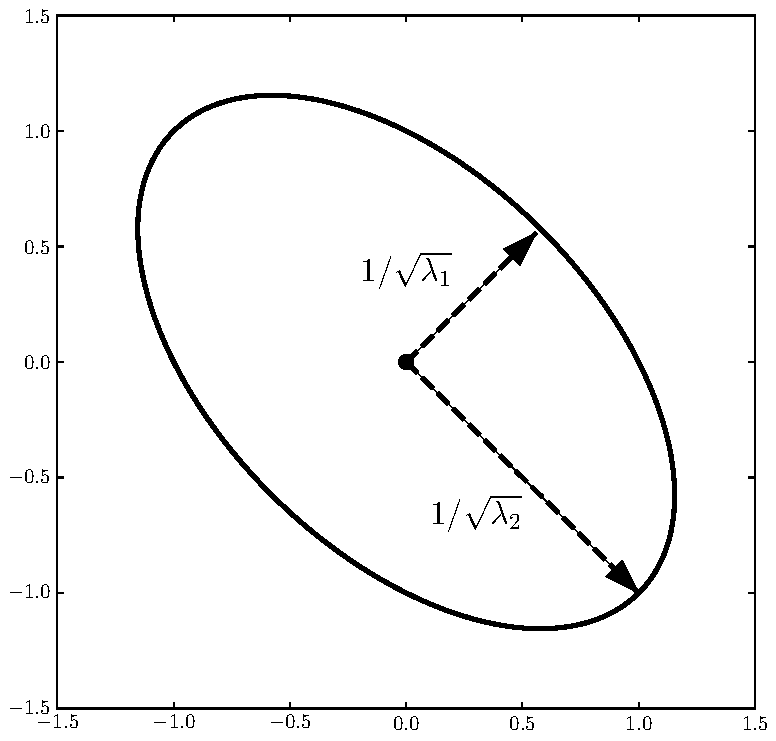
\includegraphics[width=0.7\textwidth]{i7/partiseci.7ex21.eps}
\end{center}

% QUESTION 22
\qs{I.7.22}{In the Cholesky factorization \(S = A^{\textsc{T}}A\), with \(A = \sqrt{D}L^{\textsc{T}}\), the square roots of the pivots are on the diagonal of \(A\). Find \(A\) (upper triangular) for
\[
	S = 
	\begin{bmatrix}
		9 & 0 & 0 \\
		0 & 1 & 2 \\
		0 & 2 & 8 \\
	\end{bmatrix}
	\quad
	\text{and}
	\quad
	S = 
	\begin{bmatrix}
		1 & 1 & 1 \\
		1 & 2 & 2 \\
		1 & 2 & 7 \\
	\end{bmatrix}
\]}

The \(LDL^{\textsc{T}}\) factorization is
\[
	S = 
	\begin{bmatrix}
		9 & 0 & 0 \\
		0 & 1 & 2 \\
		0 & 2 & 8 \\
	\end{bmatrix}
	=
	\begin{bmatrix}
		1 & 0 & 0 \\
		0 & 1 & 0 \\
		0 & 2 & 1 \\
	\end{bmatrix}
	\begin{bmatrix}
		9 & 0 & 0 \\
		0 & 1 & 0 \\
		0 & 0 & 4 \\
	\end{bmatrix}
	\begin{bmatrix}
		1 & 0 & 0 \\
		0 & 1 & 2 \\
		0 & 0 & 1 \\
	\end{bmatrix}
\]
Meaning that
\[
	A = \sqrt{D}L^{\textsc{T}} =
	\begin{bmatrix}
		3 & 0 & 0 \\
		0 & 1 & 0 \\
		0 & 0 & 2 \\
	\end{bmatrix}
	\begin{bmatrix}
		1 & 0 & 0 \\
		0 & 1 & 2 \\
		0 & 0 & 1 \\
	\end{bmatrix}
	=
	\begin{bmatrix}
		3 & 0 & 0 \\
		0 & 1 & 2 \\
		0 & 0 & 2 \\
	\end{bmatrix}
\]
For the second matrix, we have
\[
	S = 
	\begin{bmatrix}
		1 & 1 & 1 \\
		1 & 2 & 2 \\
		1 & 2 & 7 \\
	\end{bmatrix}
	=
	\begin{bmatrix}
		1 & 0 & 0 \\
		1 & 1 & 0 \\
		1 & 1 & 1 \\
	\end{bmatrix}
	\begin{bmatrix}
		1 & 0 & 0 \\
		0 & 1 & 0 \\
		0 & 0 & 5 \\
	\end{bmatrix}
	\begin{bmatrix}
		1 & 1 & 1 \\
		0 & 1 & 1 \\
		0 & 0 & 1 \\
	\end{bmatrix}
\]
\[
	A = \sqrt{D}L^{\textsc{T}} =
	\begin{bmatrix}
		1 & 0 & 0 \\
		0 & 1 & 0 \\
		0 & 0 & \sqrt{5} \\
	\end{bmatrix}
	\begin{bmatrix}
		1 & 1 & 1 \\
		0 & 1 & 1 \\
		0 & 0 & 1 \\
	\end{bmatrix}
\]

% QUESTION 23
\qs{I.7.23}{Suppose \(C\) is positive definite (so \(\bm{y}^{\textsc{T}}C \bm{y} > 0\) wherever \(\bm{y} \neq \bm{0}\)) and \(A\) has independent columns (so \(A \bm{x} \neq \bm{0}\) whenever \(\bm{x} \neq \bm{0}\)). Apply the energy test to \(\bm{x}^{\textsc{T}}A^{\textsc{T}}CA \bm{x}\) to show that \(\bm{S = A^{\textsc{T}}CA}\) \textbf{\textit{is positive definite: the crucial matrix in engineering.}}}

By full rank of \(A\), both \(A \bm{x}\) and \(\bm{x}^{\textsc{T}}A^{\textsc{T}}\) are nonzero for \(\bm{x} \neq \bm{0}\). By premise, \(C\) is positive definite. Therefore for any choice of \(\bm{x}\), we must have \(\!\left( \bm{x}^{\textsc{T}}A^{\textsc{T}} \right) C \!\left( A \bm{x} \right) > 0\), ascertaining that \(S = A^{\textsc{T}}CA\) is positive definite. 

\begin{center}
\centering
\textbf{The Minimum of a Function} \(\bm{F \!\left( x,y,z \right)}\)
\end{center}
What tests would you expect for a minimum point? First come zero slopes:

\noindent \textbf{First derivatives are zero} \(\displaystyle{\frac{\partial F}{\partial x} = \frac{\partial F}{\partial y} = \frac{\partial F}{\partial z} = \bm{0}}\) at the minimum point.

\noindent Next comes the linear algebra version of the usual calculus test \(d^{2}f/dx^{2} > 0\):

\noindent \textbf{Second derivative matrix \(\bm{H}\) is positive definite} \(H =
\begin{bmatrix}
	\bm{F_{xx}} & \bm{F_{xy}} & \bm{F_{xz}} \\
	\bm{F_{yx}} & \bm{F_{yy}} & \bm{F_{yz}} \\
	\bm{F_{zx}} & \bm{F_{zy}} & \bm{F_{zz}} \\
\end{bmatrix} \)

\noindent Here \(\displaystyle{\bm{F_{xy}} = \frac{\partial }{\partial x} \!\left( \frac{\partial F}{\partial y}  \right) = \frac{\partial }{\partial y} \!\left( \frac{\partial F}{\partial x}  \right) = \bm{F_{yx}}}\) is a "mixed" second derivative.

\vspace{12pt}

% QUESTION 24
\qs{I.7.24}{For \(F_{1}\!\left( x,y \right) = \frac{1}{4}x^{4} + x^{2}y + y^{2}\) and \(F_{2}\!\left( x,y \right) = x^{3} + xy - x\) find the second derivative matrices \(H_{1}\) and \(H_{2}\) (the \textbf{Hessian matrices}):
\[
	\textbf{Test for minimum } H = 
	\begin{bmatrix}
		\partial^{2}F/\partial x^{2} & \partial^{2}F / \partial x \partial y \\
		\partial^{2}F / \partial y \partial x & \partial^{2}F / \partial y^{2} \\
	\end{bmatrix} \text{is positive definite}
\]
\(H_{1}\) is positive definite so \(F_{1}\) is concave up (\(=\) convex). Find the minimum point of \(F_{1}\). \textit{Find the saddle point of} \(F_{2}\) (look only where first derivatives are zero).}

We have 
\[
	H_{1} = 
	\begin{bmatrix}
		3x^{2} + 2y & 2x \\
		2x & 2 \\
	\end{bmatrix}
\]
Take the first-order conditions:
\[
	\frac{\partial F_{1}}{\partial x} = x^{3} + 2xy = x \!\left( x^{2} + 2y \right) = 0, \quad \frac{\partial F_{1}}{\partial y} = x^{2} + 2y = 0
\]
which indicates to us that \(\min\{F_{1}\}\) corresponds to all points on the curve \(x^{2} + 2y = 0\).

For the second function, we have
\[
	H_{2} =
	\begin{bmatrix}
		6x & 1 \\
		1 & 0 \\
	\end{bmatrix}
\]
with first-order conditions
\[
	\frac{\partial F_{2}}{\partial x} = 3x^{2} + y - 1 = 0, \qquad \frac{\partial F_{2}}{\partial y} = x = 0
\]

for which \(\!\left( 0, 1 \right) \) satisfy the constraints. Then \(\det H_{2} = -1\), and the eigenvalues are \(\lambda_{1} = 1\) and \(\lambda_{2} = -1\). Since we have a positive and negative eigenvalue, we have an indefinite matrix, ascertaining that \(\!\left( 0,1 \right) \) is a saddle point.

\vspace{12pt}

% QUESTION 25
\qs{I.7.25}{Which values of \(c\) give a bowl and which \(c\) give a saddle point for the graph of \(z = 4x^{2} + 12xy + cy^{2}\)? Describe this graph at the borderline value of \(c\).}

The corresponding Hessian is
\[
	H = 
	\begin{bmatrix}
		8 & 12 \\
		12 & 2c \\
	\end{bmatrix}
\]
which is positive definite if and only if \(\det H = 16c - 144 > 0\), or equivalently, when \(c > 9\). In the case of the positive Hessian determinant, we either have two positive or two negative eigenvalues (since the determinant of a symmetric matrix is the product of the eigenvalues). When \(\det H < 0\), we must have \(c < 9\), implying a positive and negative eigenvalue, or a saddle point.

When \(c = 9\), we have \(z = \!\left( 2x + 3y \right)^{2}\). At the level \(z = 0\), we have the line \(2x + 3y = 0\). As \(z\) increases, we have a three-dimensional parabola centered on that line.

\vspace{12pt}

% QUESTION 26
\qs{I.7.26}{Without multiplying \(S = 
\begin{bmatrix}
	\cos\left( \theta  \right) & -\sin\left( \theta  \right) \\
	\sin\left( \theta  \right) & \cos\left( \theta  \right) \\
\end{bmatrix}
\begin{bmatrix}
	2 & 0 \\
	0 & 5 \\
\end{bmatrix}
\begin{bmatrix}
	\cos\left( \theta  \right) & \sin\left( \theta  \right) \\
	-\sin\left( \theta  \right) & \cos\left( \theta  \right) \\
\end{bmatrix}
\), find
\begin{enumerate}[label=(\alph*)]
	\item the determinant of \(S\)
	\item the eigenvalues of \(S\)
	\item the eigenvectors of \(S\)
	\item a reason why \(S\) is symmetric positive definite.
\end{enumerate}}

We have matrix equation \(S = Q \Lambda Q^{\textsc{T}}\).

(a) Since the determinant of a product of matrices is the product of the determinants, we have 
\[
	\det Q \Lambda Q^{\textsc{T}} = \det Q \cdot \det \Lambda \cdot \det Q^{\textsc{T}} = 10
\]
In the alternative, \(S\) is symmetric, its determinant is \(\lambda_{1}\lambda_{2} = 10\). (see (b))

(b) Since \(S\) and \(\Lambda\) are similar, they share eigenvalues. Thus \(\lambda_{1} = 2\) and \(\lambda_{2} = 5\).

(c) By the Spectral Theorem, the columns of \(Q\) are our orthogonal eigenvectors. The longer route is to observe that for \(S = Q \Lambda Q^{\textsc{T}}\), if \(\lambda\) is an eigenvalue of \(S\) and \(\bm{x}\) an eigenvector of \(S\), we have
\[
	S \bm{x} = Q \Lambda \!\left( Q^{\textsc{T}} \bm{x} \right) = \lambda \bm{x} \quad \implies \quad \Lambda \!\left( Q^{\textsc{T}}\bm{x} \right) = \lambda \!\left( Q^{\textsc{T}}\bm{x} \right) 
\]
From which we can conclude that \(Q^{\textsc{T}}\bm{x}\) is an eigenvector of \(\Lambda\). The eigenvectors \(\bm{y}\) of \(\Lambda\) are
\[
	\bm{y}_{1} = 
	\begin{bmatrix}
		1 \\
		0 \\
	\end{bmatrix},
	\quad
	\bm{y}_{2} =
	\begin{bmatrix}
		0 \\
		1 \\
	\end{bmatrix}
\]
Meaning that the eigenvectors of \(S\) are of form \(\bm{x} = Q \bm{y}\). Thus we have
\[
	\bm{x}_{1} = 
	\begin{bmatrix}
		\cos\left( \theta  \right) \\
		\sin\left( \theta  \right) \\
	\end{bmatrix},
	\quad
	\bm{x}_{2} = 
	\begin{bmatrix}
		-\sin\left( \theta  \right) \\
		\cos\left( \theta  \right) \\
	\end{bmatrix}
\]

(d) By Problem 23, since \(\Lambda\) is positive definite, so must \(S\).

\vspace{12pt}

% QUESTION 27
\qs{I.7.27}{For which \(a\) and \(c\) is this matrix positive definite? For which \(a\) and \(c\) is it positive semidefinite (this includes definite)?
\[
	S = 
	\begin{bmatrix}
		a & a & a \\
		a & a + c & a - c \\
		a & a - c & a + c \\
	\end{bmatrix}
\]
\[
	\text{All 5 tests are possible.}
\]
\[
	\text{The energy } \bm{x}^{\textsc{T}}S \bm{x} \text{ equals } a \!\left( x_{1} + x_{2} + x_{3} \right)^{2} + c \!\left( x_{2} - x_{3} \right)^{2}
\]}

Consider the vector where \(x_{2} = x_{3}\) and \(x_{1} = -2x_{2}\). Then \(\bm{x}^{\textsc{T}}S \bm{x} = 0\) for all values of \(a\) and \(c\).

For positive semidefinite, we relax the constraint to include equality: \(a \ge 0\) and \(c \ge 0\).

\vspace{12pt}

% QUESTION 28
\qs{I.7.28}{\textbf{Important!} Suppose \(S\) is positive definite with eigenvalues \(\lambda_{1} \ge \lambda_{2} \ge \cdots \ge \lambda_{n}\).
\begin{enumerate}[label=(\alph*)]
	\item What are the eigenvalues of the matrix \(\lambda_{1}I - S\)? Is it positive semidefinite?
	\item How does it follow that \(\lambda_{1}\bm{x}^{\textsc{T}}\bm{x} \ge \bm{x}^{\textsc{T}}S \bm{x}\) for every \(\bm{x}\)?
	\item Draw this conclusion: \textbf{The maximum value of } \(\bm{x}^{\textsc{T}}\bm{S} \bm{x} / \bm{x}^{\textsc{T}}\bm{x}\) \textbf{ is } \(\lambda_{1}\).
\end{enumerate}
\textit{Note}: Another way to \textbf{28}(c): \textbf{Maximize } \(\bm{x}^{\textsc{T}}\bm{S}\bm{x}\) subject to the condition \(\bm{x}^{\textsc{T}}\bm{x} = \bm{1}\). This leads to \(\displaystyle{\frac{\partial }{\partial \bm{x}}} \!\left[ \bm{x}^{\textsc{T}} \bm{S}\bm{x} - \lambda \!\left( \bm{x}^{\textsc{T}}\bm{x} - 1 \right)  \right] = \bm{0}\) and then \(S \bm{x} = \lambda \bm{x}\) and \(\lambda = \lambda_{1}\).}

(a) Consider the equation
\[
	\!\left( \lambda_{1}I - S \right) \bm{x}_{1} = \lambda_{1}\bm{x}_{1} - \lambda_{1} \bm{x}_{1} = 0 \bm{x}_{1}
\]
In general, for any eigenvector \(\bm{x}_{i}\), we have
\[
	\!\left( \lambda_{1}I - S \right) \bm{x}_{i} = \lambda_{1} \bm{x}_{i} - \lambda_{i} \bm{x}_{i} = \!\left( \lambda_{1} - \lambda_{i} \right) \bm{x}_{i}
\]
Indicating that the eigenvalues are \(\lambda_{1} - \lambda_{i}\), \(i \in \!\left\{ 1, \ldots, n \right\} \). The matrix is positive semidefinite, as \(\lambda_{1} - \lambda_{i} \ge 0\) for all \(i\). 

(b) Observe that \(\bm{x}^{\textsc{T}}S \bm{x}\) can take on values \(\lambda_{1}\bm{x}^{\textsc{T}}\bm{x}, \ldots, \lambda_{n}\bm{x}^{\textsc{T}}\bm{x}\). By premise, \(\lambda_{1} \ge \lambda_{i}\), establishing the desired inequality. 

(c) Dividing both sides of the inequality in (b) by \(\bm{x}^{\textsc{T}}\bm{x}\) (which is permissible since we mandate \(\bm{x} \neq 0\)), we deduce
\[
	\max \!\left\{ \frac{\bm{x}^{\textsc{T}}S \bm{x}}{\bm{x}^{\textsc{T}}\bm{x}} \right\} = \lambda_{1}
\]

By Lagrangian optimization, we may also maximize, subject to the condition \(\bm{x}^{\textsc{T}}\bm{x} = 1\):
\[
	\frac{\partial }{\partial \bm{x}} \!\left[ \bm{x}^{\textsc{T}}S \bm{x} - \lambda \!\left( \bm{x}^{\textsc{T}}\bm{x} - 1 \right)  \right] = 2 S \bm{x} - 2 \lambda \bm{x} = \bm{0}
\]
Implying \(S \bm{x} = \lambda \bm{x}\); invoking the premise that \(\max\{\lambda_{i}\} = \lambda_{1}\) finishes the proof.

\vspace{12pt}

\newpage
\subsection{\textsf{I.8 - Singular Values and Singular Vectors in the SVD}}

% QUESTION 1
\qs{I.8.1}{A symmetric matrix \(S = S^{\textsc{T}}\) has orthonormal eigenvectors \(\bm{v}_{1}\) to \(\bm{v}_{n}\). Then any vector \(\bm{x}\) can be written as a combination \(\bm{x} = c_{1}\bm{v}_{1} + \cdots + c_{n}\bm{v}_{n}\). Explain these two formulas:
\[
	\bm{x}^{\textsc{T}}\bm{x} = c_{1}^{2} + \cdots + c_{n}^{2} \qquad \bm{x}^{\textsc{T}}S \bm{x} = \lambda_{1} c_{1}^{2} + \cdots + \lambda_{n} c_{n}^{2}
\]}

Each term \(\!\left( \bm{x}^{\textsc{T}}\bm{x} \right)_{i} = c_{i}^{2} \bm{v}_{i}^{\textsc{T}}\bm{v}_{i} = c_{i}^{2}\) by orthonormality of the eigenvectors. 

In the second equation, we have
\[
	S \bm{x} = \lambda_{1}\bm{v}_{1} + \cdots + \lambda_{2}\bm{v}_{n}
\]
and it follows that each term \(\!\left( \bm{x}^{\textsc{T}}S \bm{x} \right)_{i} = \lambda_{i}c_{i}^{2} \bm{v}_{i}^{\textsc{T}}\bm{v} = \lambda_{i}c_{i}^{2}\), once again by orthonormality of the eigenvectors.

\vspace{12pt}

% QUESTION 2
\qs{I.8.2}{Problem 1 gives a neat form for the Rayleigh quotient \(\bm{x}^{\textsc{T}}S \bm{x} / \bm{x}^{\textsc{T}}\bm{x}\):
\[
	\boxed{R \!\left( \bm{x} \right) = \frac{\bm{x}^{\textsc{T}}S \bm{x}}{\bm{x}^{\textsc{T}}\bm{x}} = \frac{\lambda_{1}c_{1}^{2} + \cdots + \lambda_{n}c_{n}^{2}}{c_{1}^{2} + \cdots + c_{n}^{2}}}
\]
\textbf{Why is the maximum value of that ratio equal to the largest eigenvalue} \(\bm{\lambda_{1}}\) \textbf{?} This may be the simplest way to understand the "second construction" of the SVD in equation (15). You can see why thte ratio \(R \!\left( \bm{x} \right) \) is a maximum when \(c_{1} = 1\) and \(c_{2} = c_{3} = \cdots = c_{n} = 0\).
}

In the numerator, distribute out \(\lambda_{1}\) (assume it is the largest eigenvalue):
\[
	\lambda_{1} \frac{c_{1}^{2} + \frac{\lambda_{2}}{\lambda_{1}}c_{2}^{2} + \cdots + \frac{\lambda_{n}}{\lambda_{1}}c_{n}^{2}}{c_{1}^{2} + \cdots + c_{n}^{2}}
\]
By assumption, we must have \(\lambda_{j} / \lambda_{1} \le 1\) for all \(j \in \!\left\{ 2, \ldots, n \right\} \). The following inequality must immediately follow:
\[
	c_{1}^{2} + \frac{\lambda_{2}}{\lambda_{1}}c_{2}^{2} + \cdots + \frac{\lambda_{n}}{\lambda_{1}}c_{n}^{2} \le c_{1}^{2} + \cdots + c_{n}^{2}
\]
Ergo, the Rayleigh quotient is maximized when the equality holds, meaning \(R \!\left( \bm{x} \right) = \lambda_{1}\).

\vspace{12pt}

% QUESTION 3
\qs{I.8.3}{Next comes \(\lambda_{2}\) when \(\bm{x} = \bm{v}_{2}\). We maximize \(R \!\left( \bm{x} \right) = \bm{x}^{\textsc{T}}S \bm{x} / \bm{x}^{\textsc{T}}\bm{x}\) under the condition that \(\bm{x}^{\textsc{T}}\bm{v}_{1} = 0\). \textit{What does this condition mean for} \(c_{1}\)? Why is the ratio in Problem 2 now maximized when \(c_{2} = 1\) and \(c_{1} = c_{3} = \cdots = c_{n} = 0\)?}

Every \(\bm{x}\) can be written in the linear combination of eigenvectors:
\[
	\bm{x} = c_{1} \bm{v}_{1} + \cdots + c_{n} \bm{v}_{n}
\]
The constraint that \(\bm{x}^{\textsc{T}}\bm{v}_{1} = c_{1} \bm{v}_{1}^{\textsc{T}}\bm{v}_{1} = 0\) forces \(c_{1} = 0\). Proceed in the same manner as in the preceding problem: distribute out \(\lambda_{2}\), establish the same inequality between the numerator and denominator, and conclude that the ratio is maximized with equality.

\vspace{12pt}

% QUESTION 4
\qs{I.8.4}{Following Problem 3, what maximum problem is solved by \(\bm{x} = \bm{v}_{3}\)? The best \(\bm{c}\)'s are \(c_{3} = 1\) and \(c_{1} = c_{2} = c_{4} = \cdots = 0\).

The maximum of \(R \!\left( \bm{x} \right) = \displaystyle{\frac{\bm{x}^{\textsc{T}}S \bm{x}}{\bm{x}^{\textsc{T}}\bm{x}}}\) is \(\bm{\lambda}_{3}\) subject to what two conditions on \(\bm{x}\)?}

We maximize the Rayleigh quotient subject to the constraints \(\bm{x}^{\textsc{T}}\bm{v}_{1} = \bm{x}^{\textsc{T}}\bm{v}_{2} = 0\). Appeal to the logic in the preceding question, this time forcing \(c_{1} = c_{2} = 0\).

\vspace{12pt}

% QUESTION 5
\qs{I.8.5}{Show that \(A^{\textsc{T}}\) as the same (nonzero) singular values as \(A\). Then \(\abs{\abs{A}} = \abs{\abs{A^{\textsc{T}}}}\) for all matrices. But it's not true that \(\abs{\abs{A \bm{x}}} = \abs{\abs{A^{\textsc{T}}\bm{x}}}\) for all vectors. That needs \(A^{\textsc{T}}A = AA^{\textsc{T}}\).}

Let \(A = U \Sigma V^{\textsc{T}}\). Then \(A^{\textsc{T}} = V \Sigma^{\textsc{T}} U^{\textsc{T}} = V \Sigma U^{\textsc{T}}\). The matrix of singular values \(\Sigma\) is \textit{exactly} the same -- the only difference is \(A \bm{x}\) rotates \(\bm{x}\) by \(V^{\textsc{T}}\), stretches by \(\Sigma\), and rotates again by \(U\), and \(A^{\textsc{T}}\bm{x}\) rotates by \(U^{\textsc{T}}\), stretches by \(\Sigma\), and rotates once more by \(V\).

\vspace{12pt}

% QUESTION 6
\qs{I.8.6}{Find the \(\sigma\)'s and \(\bm{v}\)'s and \(\bm{u}\)'s in the SVD for \(A = 
\begin{bmatrix}
	3 & 4 \\
	0 & 5 \\
\end{bmatrix}
\). Use equation (12).}

From Example 1, observe that the \(A\) here is the transpose of the \(A\) from the example. Thus if \(A = U \Sigma V^{\textsc{T}}\), then \(A^{\textsc{T}} = V \Sigma U^{\textsc{T}}\) (in other words, switching \(U\) and \(V\)), and \(A^{\textsc{T}}A\) and \(AA^{\textsc{T}}\) are
\begin{align*}
	A^{\textsc{T}}A & =
	\begin{bmatrix}
		9 & 12 \\
		12 & 41 \\
	\end{bmatrix} \\
	AA^{\textsc{T}} & =
	\begin{bmatrix}
		25 & 20 \\
		20 & 25 \\
	\end{bmatrix}
\end{align*}

From equation (12), we can conclude that the SVD (and the new \(U\) and \(V\)) is
\[
	U = \frac{1}{\sqrt{2}}
	\begin{bmatrix}
		1 & -1 \\
		1 & 1 \\
	\end{bmatrix}
	\qquad
	\Sigma =
	\begin{bmatrix}
		\sqrt{45} & 0 \\
		0 & \sqrt{5} \\
	\end{bmatrix}
	\qquad
	V = \frac{1}{\sqrt{10}}
	\begin{bmatrix}
		1 & -3 \\
		3 & 1 \\
	\end{bmatrix}
\]

% QUESTION 7
\qs{I.8.7}{What is the norm \(\abs{\abs{A - \sigma_{1} \bm{u}_{1}\bm{v}_{1}^{\textsc{T}}}}\) when that largest rank one piece of \(A\) is removed? What are all the singular values of this reduced matrix, and its rank?}

From the following chapter, we have the following definitions for matrix norms:

\textbf{Spectral norm:} \(\abs{\abs{A}}_{2} = \sigma_{2}\)

\textbf{Frobenius norm:} \(\abs{\abs{A}}_{F} = \sqrt{\sum_{i=2}^{r} \sigma_{i}^{2}}\)

\textbf{Nuclear norm:} \(\abs{\abs{A}}_{N} = \sum_{i=2}^{r} \sigma_{i}\)

The singular values are \(\sigma_{2}, \ldots, \sigma_{r}\), which corresponds to \(\text{rank } A = r - 1\).

\vspace{12pt}

% QUESTION 8
\qs{I.8.8}{Find the \(\sigma\)'s and \(\bm{v}\)'s and \(\bm{u}\)'s, and verify that \(A = 
\begin{bmatrix}
	0 & 2 & 0 \\
	0 & 0 & 3 \\
	0 & 0 & 0 \\
\end{bmatrix} = U \Sigma V^{\textsc{T}}\). For this matrix, the orthogonal matrices \(U\) and \(V\) are permutation matrices.}

We have 
\begin{align*}
	A^{\textsc{T}}A & =
	\begin{bmatrix}
		0 & 0 & 0 \\
		0 & 4 & 0 \\
		0 & 0 & 9 \\
	\end{bmatrix} \\
	AA^{\textsc{T}} & =
	\begin{bmatrix}
		4 & 0 & 0 \\
		0 & 9 & 0 \\
		0 & 0 & 0 \\
	\end{bmatrix} \\
\end{align*}
where the former has nonzero eigenvalues \(\sigma_{1,2,3}^{2} = 0, 4, 9\) and eigenvectors (\(\bm{v}\)'s)
\[
	v_{1} = 
	\begin{bmatrix}
		1 \\
		0 \\
		0 \\
	\end{bmatrix}
	\quad
	\bm{v}_{2} =
	\begin{bmatrix}
		0 \\
		1 \\
		0 \\
	\end{bmatrix}
	\quad
	\bm{v}_{3} =
	\begin{bmatrix}
		0 \\
		0 \\
		1 \\
	\end{bmatrix}
\]
and the latter with corresponding eigenvalues \(\sigma_{1,2,3}^{2} = 4, 9, 0\) and \(\bm{u}\)'s 
\[
	\bm{u}_{1} =
	\begin{bmatrix}
		1 \\
		0 \\
		0 \\
	\end{bmatrix}
	\quad
	\bm{u}_{2} = 
	\begin{bmatrix}
		0 \\
		1 \\
		0 \\
	\end{bmatrix}
	\quad
	\bm{u}_{3} = 
	\begin{bmatrix}
		0 \\
		0 \\
		1 \\
	\end{bmatrix}
\]

Giving us SVD
\[
	\begin{bmatrix}
		0 & 2 & 0 \\
		0 & 0 & 3 \\
		0 & 0 & 0 \\
	\end{bmatrix}
	=
	\begin{bmatrix}
		0 & 1 & 0 \\
		1 & 0 & 0 \\
		0 & 0 & 1 \\
	\end{bmatrix}
	\begin{bmatrix}
		3 & 0 & 0 \\
		0 & 2 & 0 \\
		0 & 0 & 0 \\
	\end{bmatrix}
	\begin{bmatrix}
		0 & 0 & 1 \\
		0 & 1 & 0 \\
		1 & 0 & 0 \\
	\end{bmatrix}
\]
% QUESTION 9
\qs{I.8.9}{To maximize \(\bm{x}^{\textsc{T}}S \bm{x}\) with \(\bm{x}^{\textsc{T}}\bm{x} = 1\), Lagrange would work with \(L = \bm{x}^{\textsc{T}}S \bm{x} + \lambda \!\left( \bm{x}^{\textsc{T}}\bm{x} - 1 \right) \). Show that \(\bm{\nabla L} = \!\left( \partial L/ \partial x_{1}, \ldots, \partial L / \partial x_{n} \right) = 0\) is exactly \(2S \bm{x} = 2 \lambda \bm{x}\). Once again \(\max \bm{R \!\left( x \right) } = \lambda_{1}\).}

As a toy example, consider the \(2 \times 2\) case:
\[
	\bm{x}^{\textsc{T}}S \bm{x} =
	\begin{bmatrix}
		x_{1} & x_{2} \\
	\end{bmatrix}
	\begin{bmatrix}
		S_{11} & S_{12} \\
		S_{21} & S_{22} \\
	\end{bmatrix}
	\begin{bmatrix}
		x_{1} \\
		x_{2} \\
	\end{bmatrix}
	=
	x_{1}^{2} S_{11} + x_{1}x_{2} \!\left( S_{12} + S_{21} \right) + x_{2}^{2} S_{22}
\]
where \(S_{12} = S_{21}\). Derive the first-order conditions
\[
	\frac{\partial \bm{x}^{\textsc{T}}S \bm{x}}{\partial x_{1}} = 2x_{1}S_{11} + 2x_{2}S_{12} \qquad \frac{\partial \bm{x}^{\textsc{T}}S \bm{x}}{\partial x_{2}} = 2x_{2}S_{22} + 2x_{1}S_{21} 
\]
Looking at \(\bm{x}^{\textsc{T}}\bm{x}\), we have
\[
	\bm{x}^{\textsc{T}}\bm{x} = x_{1}^{2} + x_{2}^{2}
\]
which has first-order conditions
\[
	\frac{\partial \bm{x}^{\textsc{T}}\bm{x}}{\partial x_{1}} = 2x_{1} \qquad \frac{\partial \bm{x}^{\textsc{T}}\bm{x}}{\partial x_{2}} = 2x_{2}
\]
In general, for the \(n \times n\) case, we have
\[
	\bm{x}^{\textsc{T}}S \bm{x} = \sum_{i=1}^{n} x_{i}^{2} S_{ii} + \sum_{j=1}^{n} \sum_{\substack{k \neq j \\ k \in \!\left\{ 1, \ldots, n \right\} }} 2 x_{j} x_{k} S_{jk} \qquad \qquad \bm{x}^{\textsc{T}}\bm{x} = \sum_{i=1}^{n} x_{i}^{2}
\]
and first-order conditions
\[
	\frac{\partial \bm{x}^{\textsc{T}}S\bm{x}}{\partial x_{i}}  = 2x_{i} S_{ii} + \sum_{\substack{j \neq i \\ j \in \!\left\{ 1, \ldots, n \right\} }} 2 x_{j} S_{ij} \qquad \qquad \frac{\partial \bm{x}^{\textsc{T}}\bm{x}}{\partial x_{i}}  = \sum_{i=1}^{n} 2x_{i}
\]

From which we can conclude we have the following differentiation of the terms
\[
	\frac{d }{d \bm{x}} \!\left( \bm{x}^{\textsc{T}}S \bm{x} \right) = 2 S \bm{x} \qquad \frac{d }{d \bm{x}} \!\left( \bm{x}^{\textsc{T}}\bm{x} \right) = 2 \bm{x}
\]
and thus we derive the equation \(2 S \bm{x} = 2 \lambda \bm{x}\). Now, let \(\bm{x}_{i}\) be an eigenvector of \(S\) corresponding to eigenvalue \(\lambda_{i}\). It follows that
\[
	S \bm{x}_{i} - \lambda_{i}\bm{x}_{i} = \bm{0}
\]
If \(\bm{x}_{i}\) corresponds to the largest eigenvalue \(\max \lambda_{i} = \lambda_{1}\), then we have \(\max R \!\left( \bm{x} \right) = \lambda_{1}\).

\vspace{12pt}

\newpage
% QUESTION 10
\qs{I.8.10}{Prove \(\abs{\abs{B}} \le \abs{\abs{A}}\) in equation (22) by a slightly different approach. Remove first the \(N - n\) columns of \(A\). The new matrix has \(\abs{\abs{C}} \le \abs{\abs{A}}\). (Why?) Then transpose \(C\): no change in norm. Finally remove \(M - m\) columns of \(C^{\textsc{T}}\) to produce \(B^{\textsc{T}}\) with no increase in norm. Altogether \(\abs{\abs{B}} = \abs{\abs{B^{\textsc{T}}}} \le \abs{\abs{C^{\textsc{T}}}} = \abs{\abs{C}} \le \abs{\abs{A}}\).}

One intuition is by removing rows and columns, we are effectively removing "information" from the matrix. The proof is analogous to that of equation (22): if you take the vectors \(\bm{y}\) with nonzero eigenvalues, we do not increase any of the eigenvalues, and thus we cannot increase the norm. We merely take the transpose of the submatrix to remove the rows (the columns of \(C^{\textsc{T}}\), leading to the desired result.

\vspace{12pt}

% QUESTION 11

\qs{I.8.11}{Check that the trace of \(S = 
\begin{bmatrix}
	0 & A \\
	A^{\textsc{T}} & 0 \\
\end{bmatrix}
\) from adding up its diagonal entries agrees with the sum of its eigenvalues in equation (21). If \(A\) is a square diagonal matrix with entries \(1, 2, \ldots, n\), what are the \(2n\) eigenvalues and eigenvectors of \(S\)?}

We have \(\text{trace }S = 0 = \sigma_{k} - \sigma_{k}\). The eigenvectors are
\[
	\begin{bmatrix}
		\bm{u}_{k} \\
		\bm{v}_{k} \\
	\end{bmatrix}
	\qquad
	\begin{bmatrix}
		-\bm{u}_{k} \\
		\bm{v}_{k} \\
	\end{bmatrix}
\]
where \(\bm{u}_{k}\) and \(\bm{v}_{k}\) correspond to the \(k\)-th column of \(I_{n \times n}\). They have corresponding eigenvalues \(1, \ldots, n, -1, \ldots, -n\). Since \(S\) is symmetric, the eigenvalues sum to zero, as expected.

\vspace{12pt}

% QUESTION 12
\qs{I.8.12}{Find the SVD of the rank 1 matrix \(A = 
\begin{bmatrix}
	2 & 4 \\
	1 & 2 \\
\end{bmatrix}
\). Factor \(A^{\textsc{T}}A\) into \(Q \Lambda Q^{\textsc{T}}\).}

We have
\[
	A^{\textsc{T}}A = 
	\begin{bmatrix}
		5 & 10 \\
		10 & 20 \\
	\end{bmatrix}
	\qquad
	AA^{\textsc{T}} = 
	\begin{bmatrix}
		20 & 10 \\
		10 & 5 \\
	\end{bmatrix}
\]
where \(A^{\textsc{T}}A\) has eigenvectors
\[
	\bm{v}_{1} =
	\begin{bmatrix}
		1 \\
		2 \\
	\end{bmatrix}
	\qquad
	\bm{v}_{2} = 
	\begin{bmatrix}
		-2 \\
		1 \\
	\end{bmatrix}
\]
corresponding to eigenvalues \(\sigma_{1}^{2} = 25\) and \(\sigma_{2}^{2} = 0\). For those eigenvalues, in \(AA^{\textsc{T}}\) we have corresponding eigenvectors
\[
	\bm{u}_{1} =
	\begin{bmatrix}
		2 \\
		1 \\
	\end{bmatrix}
	\qquad
	\bm{u}_{2} =
	\begin{bmatrix}
		-1 \\
		2 \\
	\end{bmatrix}
\]
Giving us SVD
\[
	U =
	\begin{bmatrix}
		2 & -1 \\
		1 & 2 \\
	\end{bmatrix}
	\qquad
	\Sigma =
	\begin{bmatrix}
		5 & 0 \\
		0 & 0 \\
	\end{bmatrix}
	\qquad
	V = 
	\begin{bmatrix}
		1 & -2 \\
		2 & 1 \\
	\end{bmatrix}
\]
Now, note that \(A^{\textsc{T}}A = V \Sigma^{2} V^{\textsc{T}}\). In \(Q \Lambda Q^{\textsc{T}}\) form, we have
\[
	Q =
	\begin{bmatrix}
		1 & -2 \\
		2 & 1 \\
	\end{bmatrix}
	\qquad
	\Lambda = 
	\begin{bmatrix}
		25 & 0 \\
		0 & 0 \\
	\end{bmatrix}
	\qquad
	Q^{\textsc{T}} =
	\begin{bmatrix}
		1 & 2 \\
		-2 & 1 \\
	\end{bmatrix}
\]

% QUESTION 13
\qs{I.8.13}{Here is my homemade proof of the SVD. Step \textbf{2} uses the factorizations \(A^{\textsc{T}}A = V \Lambda V^{\textsc{T}}\) and \(AA^{\textsc{T}} = U \Lambda U^{\textsc{T}}\) (same eigenvalues in \(\Lambda\)).
\begin{alignat*}{3}
	\textbf{1} \qquad & A \!\left( A^{\textsc{T}}A \right)  && = \!\left( AA^{\textsc{T}} \right) A \\
	\textbf{2} \qquad & AV \Lambda V^{\textsc{T}} && = U \Lambda U^{\textsc{T}}A \\
	\textbf{3} \qquad & \!\left( U^{\textsc{T}}AV \right) \Lambda && = \Lambda \!\left( U^{\textsc{T}}AV \right) \\
	\textbf{4} \qquad & U^{\textsc{T}}AV && \text{ must be diagonal}  
\end{alignat*}
Step 3 multiplied Step 2 on the left by \underline{\qquad} and on the right by \underline{\qquad}. Then the matrix \(U^{\textsc{T}}AV\) commutes with the diagonal matrix \(\Lambda\) in Step 3. How does this force the matrix \(U^{\textsc{T}}AV = \Sigma\) to be also a diagonal matrix? Try 3 by 3.
\[\resizebox{1\hsize}{!}{\(
	\bm{\Sigma \Lambda} = 
	\begin{bmatrix}
		\sigma_{11} & \sigma_{12} & \sigma_{13} \\
		\sigma_{21} & \sigma_{22} & \sigma_{23} \\
		\sigma_{31} & \sigma_{32} & \sigma_{33} \\
	\end{bmatrix}
	\begin{bmatrix}
		\lambda_{1} &  &  \\
		 & \lambda_{2} &  \\
		 &  & \lambda_{3} \\
	\end{bmatrix} =
	\begin{bmatrix}
		\lambda_{1} &  &  \\
		 & \lambda_{2} &  \\
		 &  & \lambda_{3} \\
	\end{bmatrix}
	\begin{bmatrix}
		\sigma_{11} & \sigma_{12} & \sigma_{13} \\
		\sigma_{21} & \sigma_{22} & \sigma_{23} \\
		\sigma_{31} & \sigma_{32} & \sigma_{33} \\
	\end{bmatrix}
	= \bm{\Lambda \Sigma}\)}
\] Compare the first rows. When can you conclude that \(\sigma_{12} = 0\) and \(\sigma_{13} = 0\)? This shows the limitation on my proof: \textit{It needs the eigenvalues of } \(A^{\textsc{T}}A\) \textit{ to be} \underline{\qquad}.

The same bug appears in simple proofs of the spectral theorem \(S = Q \Lambda Q^{\textsc{T}}\). This is easy when \(S\) has no repeated \(\lambda\)'s. The SVD is easy when \(A\) has no repeated \(\sigma\)'s.

Both \(S = Q \Lambda Q^{\textsc{T}}\) and \(A = U \Sigma V^{\textsc{T}}\) remain true when \(\lambda\)'s or \(\sigma\)'s happen to be repeated. The problem is that this produces a whole plane of eigenvectors or singular vectors. You have to choose the singular vectors \(\bm{u}\) specifically as \(A \bm{v} / \sigma\) -- which is the real proof in equation (9).}

In step 3, we left-multiply by \(U^{\textsc{T}}\) and right-multiply by \(V\). In the 3 by 3 case given, the first rows have
\[
	\begin{bmatrix}
		\lambda_{1}\sigma_{11} & \lambda_{2}\sigma_{12} & \lambda_{3}\sigma_{13} \\
	\end{bmatrix}
	=
	\begin{bmatrix}
		\lambda_{1}\sigma_{11} & \lambda_{1}\sigma_{12} & \lambda_{1}\sigma_{13} \\
	\end{bmatrix}
\]
where we must require that -- in order for the equality to hold -- the eigenvalues of \(A^{\textsc{T}}A\) be \textit{unique} to conclude that all non-diagonal entries of \(\Sigma\) are zero. 

\vspace{12pt}

% QUESTION 14
\qs{I.8.14}{Figure I.10 showed how a 2 by 2 matrix with four entries \(a\), \(b\), \(c\), \(d\) produces an SVD with four parameters \(\theta \), \(\phi \), \(\sigma_{1}\), \(\sigma_{2}\). Move to \(A = U \Sigma V^{\textsc{T}} =\) 2 by 3 with six entries.

How many \(\sigma\)'s for a 2 by 3 matrix? Then \(U\) (2 by 2) only needs one angle. To recover \(A\), that leaves how many angles for the 3 by 3 orthogonal matrix \(V\)?

The row space of \(A\) is a plane in \(\mathbb{R}^{3}\). It takes \underline{\qquad} angles for the position of that plane. It takes \underline{\qquad} angle in the plane to find \(\bm{v}_{1}\) and \(\bm{v}_{2}\). A total of \underline{\qquad} angles for \(V\).}

We have two \(\sigma\)'s. The matrix \(V\) requires three angles: two angles to fix the position of the plane, and one angle to find \(\bm{v}_{1}\) and \(\bm{v}_{2}\) in the plane. 

\vspace{12pt}

% QUESTION 15
\qs{I.8.15}{Every 3 by 3 matrix has 9 entries. So \(U \Sigma V^{\textsc{T}}\) must have 9 parameters. How many parameters in \(U\) and \(\Sigma\) and \(V\)? \textit{Answer the same questions for }4 \textit{by }4. How many parameters describe a rotation in 4-dimensional space?}

We have three parameters each in \(U\), \(\Sigma\), and \(V\). In \(\mathbb{R}^{4}\), \(U\) and \(V\) each have six parameters, and four in \(\Sigma\).

\vspace{12pt}

% QUESTION 16
\qs{I.8.16}{\underline{\qquad} numbers will give the direction of a unit vector \(\bm{v}_{1}\) in \(\mathbb{R}^{5}\). Then the direction of an orthogonal unit vector \(\bm{v}_{2}\) takes \underline{\qquad} numbers. How many for \(\bm{v}_{3}\), \(\bm{v}_{4}\), \(\bm{v}_{5}\)? Total \underline{\qquad}.}

This question is a "degrees of freedom" question, which intuitively is a measure of how many choices we have given constraints. In choosing the first unit vector, observe that picking the first four numbers automatically fixes the fifth (so as to guarantee the unit vector norm). 

Moving on, once imposing the orthogonality constraint on the second unit vector, we lose a dimension. Therefore we only have three choices of numbers for \(\bm{v}_{2}\). Proceeding in this manner, we have two, one, and zero choices for \(\bm{v}_{3}\), \(\bm{v}_{4}\), and \(\bm{v}_{5}\). Summing \(4 + 3 + 2 + 1 = 10\).

\vspace{12pt}

% QUESTION 17
\qs{I.8.17}{\textbf{If \(\bm{v}\) is an eigenvector of \(\bm{A^{\textsc{T}}A}\) with \(\bm{\lambda \neq 0}\), then \underline{\qquad} is an eigenvector of \(\bm{AA^{\textsc{T}}}\)}.}

We have \(A^{\textsc{T}}A \bm{v} = \lambda \bm{v}\), which implies \(\!\left( AA^{\textsc{T}} \right) A \bm{v} = \lambda A \bm{v}\), or that \(A \bm{v}\) is an eigenvector of \(AA^{\textsc{T}}\).

\vspace{12pt}

% QUESTION 18
\qs{I.8.18}{If \(A = U \Sigma V^{\textsc{T}}\) is square and invertible, then \(A^{-1} = \) \underline{\qquad}. Find all singular values of \(A^{\textsc{T}}A\) (not of \(A\)).}

We have \(A^{-1} = V \Sigma^{-1} U^{\textsc{T}}\). The singular values of \(A^{\textsc{T}}A\) are the diagonal entries of \(\Sigma^{2}\):
\[
	A^{\textsc{T}}A = V \Sigma^{2} V^{\textsc{T}}
\]

\vspace{12pt}

% QUESTION 19
\qs{I.8.19}{If \(A = A^{\textsc{T}}\) has orthogonal columns \(\bm{u}_{1}\), \(\bm{u}_{2}\), \(\bm{u}_{3}\) in \(\mathbb{R}^{2}\) of lengths 2, 3, 4, find its SVD.}

We have
\[
	A^{\textsc{T}}A = 
	\begin{bmatrix}
		\bm{u}_{1}^{\textsc{T}} \\
		\bm{u}_{2}^{\textsc{T}} \\
		\bm{u}_{3}^{\textsc{T}} \\
	\end{bmatrix}
	\begin{bmatrix}
		\bm{u}_{1} & \bm{u}_{2} & \bm{u}_{3} \\
	\end{bmatrix} =
	\begin{bmatrix}
		4 & 0 & 0 \\
		0 & 9 & 0 \\
		0 & 0 & 16 \\
	\end{bmatrix}
\]
which has eigenvectors
\[
	\bm{v}_{1} =
	\begin{bmatrix}
		1 \\
		0 \\
		0 \\
	\end{bmatrix}
	\qquad
	\bm{v}_{2} =
	\begin{bmatrix}
		0 \\
		1 \\
		0 \\
	\end{bmatrix}
	\qquad
	\bm{v}_{3} =
	\begin{bmatrix}
		0 \\
		0 \\
		1 \\
	\end{bmatrix}
\]
corresponding to eigenvalues \(\sigma_{1,2,3}^{2} = 4, 9, 16\). The \(U\) matrix eigenvectors are
\[
	\bm{u}_{1}^{*} = \frac{A \bm{v}_{1}}{\sigma_{1}} = \frac{1}{2}\bm{u}_{1}, \quad \bm{u}_{2}^{*} = \frac{A \bm{v}_{2}}{\sigma_{2}} = \frac{1}{3}\bm{u}_{2}, \quad \bm{u}_{3}^{*} = \frac{A \bm{v}_{3}}{\sigma_{3}} = \frac{1}{4} \bm{u}_{3} 
\]
Giving us SVD
\[
	U = 
	\begin{bmatrix}
		\frac{1}{2}\bm{u}_{1} & \frac{1}{3}\bm{u}_{2} & \frac{1}{4}\bm{u}_{3} \\
	\end{bmatrix}
	\qquad
	\Sigma = 
	\begin{bmatrix}
		2 & 0 & 0 \\
		0 & 3 & 0 \\
		0 & 0 & 4 \\
	\end{bmatrix}
	\qquad
	V = 
	\begin{bmatrix}
		1 & 0 & 0 \\
		0 & 1 & 0 \\
		0 & 0 & 1 \\
	\end{bmatrix}
\]

% QUESTION 20
\qs{I.8.20}{The reasons for the success of eigenvalues and eigenvectors are in \(\bm{A^{k} = X \Lambda^{k} X^{-1}}\):
\begin{enumerate}[label=(\alph*)]
	\item The eigenvalues of \(A^{k}\) are \(\lambda_{1}^{k}, \ldots, \lambda_{n}^{k}\)
	\item An eigenvector \(\bm{x}\) of \(A\) is also an eigenvector of \(A^{k}\).
\end{enumerate}
\textbf{Show that a) and b) are false for singular values and singular vectors of} \(
\begin{bmatrix}
	-2 & -6 \\
	6 & 2 \\
\end{bmatrix}
\).}

The SVD is
\[
	\displaystyle{A = U \Sigma V^{\textsc{T}} =
	\begin{bmatrix}
		-\frac{1}{\sqrt{2}} & \frac{1}{\sqrt{2}} \\
		\frac{1}{\sqrt{2}} & \frac{1}{\sqrt{2}} \\
	\end{bmatrix}
	\begin{bmatrix}
		8 & 0 \\
		0 & 4 \\
	\end{bmatrix}
	\begin{bmatrix}
		\frac{1}{\sqrt{2}} & \frac{1}{\sqrt{2}} \\
		\frac{1}{\sqrt{2}} & -\frac{1}{\sqrt{2}} \\
\end{bmatrix}}
\]
Unfortunately, we see that \(\!\left( V^{\textsc{T}} \right)^{-1} = V \neq U\). As such, the properties of the eigendecomposition fail to hold in the case of the SVD.

\vspace{12pt}

% QUESTION 21
\qs{I.8.21}{Show that the singular values of \(AA^{\textsc{T}}A\) are \(\!\left( \sigma_{1} \right)^{3}\) to \(\!\left( \sigma_{r} \right)^{3}\).}

We have
\[
	\!\left( U \Sigma V^{\textsc{T}} \right) \!\left( V \Sigma^{2} V^{\textsc{T}} \right) = U \Sigma^{3} V^{\textsc{T}} 
\]
with diagonal entries in \(\Sigma^{3}\) equal to \(\!\left( \sigma_{1} \right)^{3}\) through \(\!\left( \sigma_{r} \right)^{3}\).

\vspace{12pt}

% QUESTION 22
\qs{I.8.22}{Equation (5) is \(AV_{r} = U_{r}\Sigma_{r}\). Multiply by \(V_{r}^{\textsc{T}}\) to get \(A = U_{r}\Sigma_{r}V_{r}^{\textsc{T}}\) (\textbf{reduced SVD}).

For that step we cannot use \(V_{r}V_{r}^{\textsc{T}} = I\) (which is false when \(m > r\)). Show instead that this matrix \(A = U_{r}\Sigma_{r}V_{r}^{\textsc{T}}\) satisfies equation (1).}

Although \(V_{r}V_{r}^{\textsc{T}} \neq I\), we certainly have \(V_{r}^{\textsc{T}}V_{r} = I\). Given \(A = U_{r}\Sigma_{r}V_{r}^{\textsc{T}}\), right-multiply by \(V_{r}\) to get \(AV_{r} = U_{r}\Sigma_{r}\). Taking the columns of \(V_{r}\) and \(U_{r}\), we see that the equations \(A \bm{v}_{i} = \sigma_{i}\bm{u}_{i}\) are consistent for \(i \in \!\left\{ 1, \ldots, r \right\} \).

Moreover, for vectors \(\bm{v}_{r + 1}, \ldots, \bm{v}_{n}\), we see that since these vectors live in \(\textbf{N}\!\left( A \right) \), we get
\[
	A \bm{v}_{k} = U_{r}\Sigma_{r}V_{r}^{\textsc{T}} \bm{v}_{k} = \bm{0}
\]

% QUESTION 23
\qs{I.8.23}{Show that an \(m\) by \(n\) matrix of rank \(r\) has \(r \!\left( m + n - r \right) \) free parameters in its SVD: \(A = U \Sigma V^{\textsc{T}} = \!\left( m \times r \right) \!\left( r \times r \right) \!\left( r \times n \right) \). Why do \(r\) orthonormal vectors \(\bm{u}_{1}\) to \(\bm{u}_{r}\) have \(\!\left( m - 1 \right) + \!\left( m - 2 \right) + \cdots + \!\left( m - r \right) \) parameters?

\vspace{12pt}

Another approach uses \(A = CR = \!\left( m \times r \right) \!\left( r \times n \right) \) from Section I.1. The matrix \(R\) contains an \(r\) by \(r\) identity matrix removing \(r^{2}\) parameters from \(rm + rn\). That count is repeated in an appendix of this book.}

Proceeding in an analogous logic to Exercise 16, we have \(m - 1\) parameters in choosing \(\bm{u}_{1}\) -- one fewer parameter than \(m\) thanks to the unit vector norm. We progressively lose a dimension to choose, up until \(m - r\) parameters for \(\bm{u}_{r}\).

For matrix \(U\), we have \(rm - r \!\left( r + 1 \right) / 2\) parameters. Similarly for matrix \(V\), we have \(rn - r \!\left( r + 1 \right) / 2\). And lastly, \(r\) parameters for \(\Sigma\). Summing the three, we get
\[
	rm + rn - r \!\left( r + 1 \right) + r = rm + rn - r^{2} = r \!\left( m + n - r \right) 
\]


\newpage
\subsection{\textsf{I.9 - Principal Components and the Best Low Rank Matrix}}

% QUESTION 1
\qs{I.9.1}{What are the singular values (in descending order) of \(\bm{A} - \bm{A_{k}}\)? Omit any zeros.}

Since \(\bm{A} = \sigma_{1}\bm{u}_{1}\bm{v}_{1}^{\textsc{T}} + \cdots + \sigma_{r}\bm{u}_{r}\bm{v}_{r}^{\textsc{T}}\) and \(\bm{A_{k}} = \sigma_{1}\bm{u}_{1}\bm{v}_{1}^{\textsc{T}} + \cdots + \sigma_{k}\bm{u}_{k}\bm{v}_{k}^{\textsc{T}}\), we have
\[
	\bm{A} - \bm{A_{k}} = \sigma_{k+1}\bm{u}_{k+1}\bm{v}_{k+1}^{\textsc{T}} + \cdots + \sigma_{r}\bm{u}_{r}\bm{v}_{r}^{\textsc{T}}
\]
which has singular values \(\sigma_{k+1} \ge \ldots \ge \sigma_{r}\).

\vspace{12pt}

% QUESTION 2
\qs{I.9.2}{Find a closest rank-1 approximation to these matrices (\(L^{2}\) or Frobenius norm):
\[
	A =
	\begin{bmatrix}
		3 & 0 & 0 \\
		0 & 2 & 0 \\
		0 & 0 & 1 \\
	\end{bmatrix}
	\qquad
	A = 
	\begin{bmatrix}
		0 & 3 \\
		2 & 0 \\
	\end{bmatrix}
	\qquad
	A = 
	\begin{bmatrix}
		2 & 1 \\
		1 & 2 \\
	\end{bmatrix}
\]}

By Eckart-Young, we have in the first matrix:
\[
	A_{1} =
	\begin{bmatrix}
		3 & 0 & 0 \\
		0 & 0 & 0 \\
		0 & 0 & 0 \\
	\end{bmatrix}
\]
The second matrix has SVD
\[
	A =
	\begin{bmatrix}
		1 & 0 \\
		0 & 1 \\
	\end{bmatrix}
	\begin{bmatrix}
		3 & 0 \\
		0 & 2 \\
	\end{bmatrix}
	\begin{bmatrix}
		0 & 1 \\
		1 & 0 \\
	\end{bmatrix}
	= \sigma_{1}\bm{u}_{1}\bm{v}_{1}^{\textsc{T}} + \sigma_{2}\bm{u}_{2}\bm{v}_{2}^{\textsc{T}}
\]
Immediately yielding
\[
	A_{1} = 
	\begin{bmatrix}
		0 & 3 \\
		0 & 0 \\
	\end{bmatrix}
\]
Lastly, the third matrix has SVD
\[
	A = 
	\begin{bmatrix}
		1/\sqrt{2} & 1/\sqrt{2} \\
		1/\sqrt{2} & -1/\sqrt{2} \\
	\end{bmatrix}
	\begin{bmatrix}
		3 & 0 \\
		0 & 1 \\
	\end{bmatrix}
	\begin{bmatrix}
		1/\sqrt{2} & 1/\sqrt{2} \\
		1/\sqrt{2} & -1/\sqrt{2} \\
	\end{bmatrix}
\]
Giving us
\[
	A_{1} = 
	\begin{bmatrix}
		3/2 & 3/2 \\
		3/2 & 3/2 \\
	\end{bmatrix}
\]

% QUESTION 3
\qs{I.9.3}{Find a closest rank-1 approximation in the \(L^{2}\) norm to \[A = 
\begin{bmatrix}
	\cos\left( \theta  \right) & -\sin\left( \theta  \right) \\
	\sin\left( \theta  \right) & \cos\left( \theta  \right) \\
\end{bmatrix}
\]}

Observe that we have repeated singular values: \(\sigma_{1} = \sigma_{2} = 1\). In this instance we see for the spectral norm that \(\max \abs{\abs{A \bm{x}}} / \abs{\abs{\bm{x}}}\) is unchanged for any choice of non-zero \(\bm{x}\): \(A\) will never stretch \(\bm{x}\), so we will always have \(\abs{\abs{A}}_{2} = 1\).

For the Frobenius norm, consider the rank 1 matrix
\[
	A_{1} = 
	\begin{bmatrix}
		\cos\left( \theta  \right) & 0 \\
		\sin\left( \theta  \right) & 0 \\
	\end{bmatrix}
\]
which we derive from the SVD \(A = AII\). Then we have
\[
	A - A_{1} =
	\begin{bmatrix}
		0 & -\sin\left( \theta  \right) \\
		0 & \cos\left( \theta  \right) \\
	\end{bmatrix}
\]
which has singular values \(\sigma_{1} = 1\) and \(\sigma_{2} = 0\). Then \(\abs{\abs{A - A_{1}}}_{F}^{2} = 1\), notably less than \(\abs{\abs{A}}_{F}^{2} = 2\).

\vspace{12pt}

% QUESTION 4
\qs{I.9.4}{The Eckart-Young theorem is false in the matrix norm \(\abs{\abs{A}}_{\infty} = \) max row sum:
\[
	A = 
	\begin{bmatrix}
		a & b \\
		c & d \\
	\end{bmatrix}
	\text{ has } \abs{\abs{A}}_{\infty} = \max \frac{\abs{\abs{A \bm{x}}}_{\infty}}{\abs{\abs{\bm{x}}}_{\infty}} = \max \!\left( \abs{a} + \abs{b}, \abs{c} + \abs{d} \right) 
\]
Find a rank-1 matrix closer to \(A = 
\begin{bmatrix}
	3 & 0 \\
	4 & 5 \\
\end{bmatrix}
\) than \(A_{1} = \displaystyle{\frac{3}{2}}
\begin{bmatrix}
	1 & 1 \\
	3 & 3 \\
\end{bmatrix}\).}

Note that this is the transpose of the matrix in exercise I.8.6. We calculate
\[
	A - A_{1} =
	\begin{bmatrix}
		3/2 & -3/2 \\
		-1/2 & 1/2 \\
	\end{bmatrix}
\]
which indicates that \(\abs{\abs{A - A_{1}}}_{\infty} = \max \!\left( 3, 1 \right) = 3\). Consider the rank 1 matrix
\[
	A_{1} = 
	\begin{bmatrix}
		a & b \\
		ca & cb \\
	\end{bmatrix}
\]
We can write code that identifies the best \(a\), \(b\), and \(c\) that minimizes \(\abs{\abs{A - A_{1}}}_{\infty}\). My Python code gives me
\[
	a = 2.97 \qquad b = 2.12 \qquad c = 1.35
\]
which yields
\[
	A - A_{1} =
	\begin{bmatrix}
		3 & 0 \\
		4 & 5 \\
	\end{bmatrix}
	-
	\begin{bmatrix}
		2.97 & 2.12 \\
		1.35 \cdot 2.97 & 1.35 \cdot 2.12 \\
	\end{bmatrix}
	=
	\begin{bmatrix}
		0.03 & -2.12 \\
		-0.0095 & 2.138 \\
	\end{bmatrix}
\]
For a matrix norm of \(\abs{\abs{A - A_{1}}} = 2.15\).

\vspace{12pt}

% QUESTION 5
\qs{I.9.5}{Show that this norm \(\abs{\abs{A}}_{\infty} = \max \!\left( \abs{a} + \abs{b}, \abs{c} + \abs{d} \right) \) is not orthogonally variant:
\[
	\text{Find a diagonal matrix } A \text{ where } \abs{\abs{QA}}_{\infty} \neq \abs{\abs{A}}_{\infty} \text{ for } 
\]

\[
	Q = 
	\begin{bmatrix}
		\cos\left( \theta  \right) & -\sin\left( \theta  \right) \\
		\sin\left( \theta  \right) & \cos\left( \theta  \right) \\
	\end{bmatrix}
\]}

Let \(a \in \mathbb{R}\). Define 
\[
	A = 
	\begin{bmatrix}
		a & 0 \\
		0 & a \\
	\end{bmatrix}
\]
Then we have
\[
	QA = 
	\begin{bmatrix}
		a \cos\left( \theta  \right) & -a \sin\left( \theta  \right) \\
		a \sin\left( \theta  \right) & a \cos\left( \theta  \right) \\
	\end{bmatrix}
\]
with norms
\[
	\abs{\abs{A}}_{\infty} = \abs{a}
\]
\[
	\abs{\abs{QA}}_{\infty} = \abs{a} \!\left( \abs{\cos\left( \theta  \right)} + \abs{\sin\left( \theta  \right)} \right) 
\]
where in general, we must have \(\abs{\abs{QA}}_{\infty} \neq \abs{\abs{A}}_{\infty}\).

\vspace{12pt}

% QUESTION 6
\qs{I.9.6}{If \(S = Q \Lambda Q^{\textsc{T}}\) is a symmetric positive definite matrix, explain from Eckart-Young why \(\bm{q }_{1} \lambda_{1}\bm{q }_{1}^{\textsc{T}}\) is the closest rank-1 approximation in the \(L^{2}\) matrix norm \(\abs{\abs{S}}_{2}\).}

Since \(S\) is symmetric positive definite, its SVD is precisely \(Q \Lambda Q^{\textsc{T}}\). By definition, the \(L^{2}\) norm is
\[
	\abs{\abs{S}}_{2} = \max \frac{\abs{\abs{S \bm{x}}}}{\abs{\abs{\bm{x}}}} = \sigma_{1}
\]
By Eckart-Young, for \(k = 1\), we have
\[
	\abs{\abs{S - \bm{q}_{1}\lambda_{1}\bm{q}_{1}^{\textsc{T}}}} = \max \frac{\abs{\abs{\!\left( S - \bm{q}_{1}\lambda_{1}\bm{q}_{1}^{\textsc{T}} \right) \bm{x}}}}{\abs{\abs{\bm{x}}}} = \lambda_{2} \ge \lambda_{2}
\]
Since Eckart-Young sets the lower bound as \(\lambda_{2}\), it must be that \(\bm{q }_{1}\lambda_{1}\bm{q }_{1}^{\textsc{T}}\) is the closest rank-1 approximation in \(L^{2}\).

\vspace{12pt}

% QUESTION 7
\qs{I.9.7}{Explain the derivatives \(\partial E / \partial C\) and \(\partial E / \partial R\) in equation (19) for size \(n = 2\).}

% QUESTION 8
\qs{I.9.8}{Which rank-3 matrices have \(\abs{\abs{A - A_{1}}}_{2} = \abs{\abs{A - A_{2}}}_{2}\)? \(A_{2}\) is \(\sigma_{1} \bm{u}_{1} \bm{v}_{1}^{\textsc{T}} + \sigma_{2}\bm{u}_{2}\bm{v}_{2}^{\textsc{T}}\).}

Since we have the \(L^{2}\) norm, we have \(\abs{\abs{A - A_{1}}}_{2} = \sigma_{2}\) and \(\abs{\abs{A - A_{2}}}_{2} = \sigma_{3}\). Consequently, matrices \(A\) that satisfy these conditions must have \(\sigma_{2} = \sigma_{3}\).

\vspace{12pt}

% QUESTION 9
\qs{I.9.9}{Replace the quarter circle Figure I.13 by the parabola \(\bm{y = 1 - x^{2}}\). Estimate the rank \(CN\) with all 1's under the parabola (\(N\) 1's along the axes). First remove a rectangle of 1's, touching the parabola where slope \(= -1\).}

% QUESTION 10
\qs{I.9.10}{If \(A\) is a 2 by 2 matrix with \(\sigma_{1} \ge \sigma_{2} > 0\), find \(\abs{\abs{A^{-1}}}_{2}\) and \(\abs{\abs{A^{-1}}}^{2}_{F}\).}

We have
\[
	\abs{\abs{A^{-1}}}_{2} = \frac{1}{\sigma_{2}} \qquad \abs{\abs{A^{-1}}}^{2}_{F} = \frac{1}{\sigma_{1}^{2}} + \frac{1}{\sigma_{2}^{2}}
\]
Intuitively, in the \(L^{2}\) norm, the singular value matrix of \(A^{-1}\) is \(\Lambda^{-1}\). Its largest singular value is \(1 / \sigma_{2}\). In the Frobenius norm, we simply have the sum of the squared diagonal entries of \(\Lambda^{-1}\).

\newpage
\subsection{\textsf{I.10 - Rayleigh Quotients and Generalized Eigenvalues}}


\end{document}
